%; whizzy paragraph
%; whizzy-paragraph "^\\\\dancersection"
% -initex iniptex -latex platex -format platex -bibtex jbibtex -fmt fmt
% $B0J>e(B whizzytex $B$r;HMQ$9$k>l9g$N@_Dj!#(B

%     Tokyo Debian Meeting resources
%     Kansai Debian Meeting resources
%     Copyright (C) 2012 Junichi Uekawa
%     Copyright (C) 2012 Nobuhiro Iwamatsu
%     Copyright (C) 2012 Koichi Akabe

%     This program is free software; you can redistribute it and/or modify
%     it under the terms of the GNU General Public License as published by
%     the Free Software Foundation; either version 2 of the License, or
%     (at your option) any later version.

%     This program is distributed in the hope that it will be useful,
%     but WITHOUT ANY WARRANTY; without even the implied warranty of
%     MERCHANTABILITY or FITNESS FOR A PARTICULAR PURPOSE.  See the
%     GNU General Public License for more details.

%     You should have received a copy of the GNU General Public License
%     along with this program; if not, write to the Free Software
%     Foundation, Inc., 51 Franklin St, Fifth Floor, Boston, MA  02110-1301 USA

%  preview (shell-command (concat "evince " (replace-regexp-in-string "tex$" "pdf"(buffer-file-name)) "&"))
% $B2hA|%U%!%$%k$r=hM}$9$k$?$a$K$O(Bebb$B$rMxMQ$7$F(Bboundingbox$B$r:n@.!#(B
%(shell-command "cd image2012-natsu; ebb *.png")

% progress memo:
% 2018/12-2019/05$BEl5~$,%^!<%8BP>](B
% 2019/07$B%j%j!<%9%Q!<%F%#%M%?$b2DG=$J$i<}O?(B
% $B%$%Y%s%HEy$G$J$$>l9g$OM}M3$r=q$/$3$H!#(B
% $BI,MW$JJQ99E@$O(B FIXME $B$G5-O?$7$F$$$^$9!#(B

%%$B$3$3$+$i%X%C%@3+;O!#(B

\documentclass[mingoth,a4paper]{jsarticle}
\usepackage{monthlyreport}
\usepackage{supertabular}
\usepackage{subfigure}
\renewcommand*\thesubfigure{}

\usepackage{comment}

% section $B$NBe$o$j$N4D6-(B -- $B2~D{$9$k!#(B
\renewcommand{\dancersection}[2]{%
\newpage
$B$"$s$I$-$e$a$s$F$C$I(B $B$G$S$"$s(B 2019$BG/2F9f(B
%
% top line
\vspace{0.1mm}\\
{\color{dancerdarkblue}\rule{\hsize}{2mm}}

%
% middle text
%
\begin{minipage}[t]{0.6\hsize}
\color{dancerdarkblue}
\vspace{1cm}
\section{#1}
\hfill{}#2\\
\end{minipage}
\begin{minipage}[t]{0.4\hsize}
\vspace{-2cm}
\hfill{}
\includegraphics[height=8cm]{image200502/openlogo-nd.eps}\\
\vspace{-5cm}
\end{minipage}
%
% bottom line
{\color{dancerlightblue}\rule{0.66\hsize}{2mm}}
%
\vspace{2cm}
}
% end of dancersection.

\begin{document}

\begin{titlepage}
\thispagestyle{empty}

\hspace*{-2.5cm}
\includegraphics{image2012-natsu/gudeb.eps}\\
\vspace*{0.1cm}

\vspace*{2cm}
\rotatebox{10}{\fontsize{32}{32} {\gt $BEl5~%(%j%"(B/$B4X@>#D#e#b#i#a#nJY6/2q(B}}

\vspace*{-1.5cm}
\hspace*{11cm}
\includegraphics[height=6cm]{image200502/openlogo-nd.eps}\\
\vspace*{0.1cm}
\hfill $B$"$s$I$-$e$a$s$F$C$I(B $B$G$S$"$s(B 2019$BG/2F9f(B 2019$BG/(B8$B7n(B12$BF|(B $B=iHGH/9T(B
\end{titlepage}

\newpage
\thispagestyle{empty}\mbox{}
\newpage

\setcounter{page}{1}
\begin{minipage}[]{0.2\hsize}
 \definecolor{titleback}{gray}{0.9}
 \colorbox{dancerlightblue}{\rotatebox{90}{\fontsize{80}{80}
{\gt \color{dancerdarkblue}$B%G%S%"%sJY6/2q(B} }}
\end{minipage}
\begin{minipage}[]{0.8\hsize}
\hrule
\vspace{1mm}
\hrule
\setcounter{tocdepth}{1}
{\small
\begin{multicols}{2}
  \tableofcontents
\end{multicols}
} %FIXME: does not fit in one column! $B$7$+$7FsCJ$K$9$k$H$"$^$jH~$7$/$J$$!)(B $B??$sCf$N$"$?$j$G>OHV9f$H%Z!<%8?t$NHV9f$,6a$/$K$"$k$N$,%P%i%s%9NI$/$J$$5$$,$9$k(B
\vspace{1mm}
\hrule
\vspace{3cm}

\end{minipage}

% FIXME: $BK\J8$rDI2C$9$k$3$H!#(B
%-------------------------------------------------------------------------------
\dancersection{Introduction}{ }
%-------------------------------------------------------------------------------

\subsection{$BEl5~%(%j%"(BDebian$BJY6/2q(B}

 Debian$BJY6/2q$X$h$&$3$=!#$3$l$+$i(BDebian$B$N@$3&$K$"$7$rF'$_F~$l$k$H(B
 $B$$$&J}$b!"$9$G$K$I$C$W$j$H$D$+$C$F$$$k$H$$$&J}$b!"7n$K0l2s(BDebian$B$K$D$$(B
 $B$F8l$j$^$;$s$+!)(B

 Debian$BJY6/2q$NL\E*$O2<5-$G$9!#(B

\begin{itemize}
 \item \underline{Debian Developer} ($B3+H/<T(B)$B$N0i@.!#(B
 \item $BF|K\8l$G$N!V(B\underline{$B3+H/$K4X$9$k>pJs(B}$B!W$r@0M}$7$F$^$H$a!"%"%C%W%G!<%H$9$k!#(B
 \item \underline{$B>l(B}$B$NDs6!!#(B
 \begin{itemize}
  \item $BIaCJ$P$i$P$i$J>l=j$K$$$k?M!9$,(B face-to-face $B$G=P2q$($k>l$rDs6!(B
	$B$9$k!#(B
  \item Debian $B$N$?$a$K$J$k$3$H$r8l$k>l$rDs6!$9$k!#(B
  \item Debian$B$K$D$$$F8l$k>l$rDs6!$9$k!#(B
 \end{itemize}
\end{itemize}

 Debian$B$NJY6/2q$H$$$&$3$H$G5f6KE*$K$O;22C<TA40w$,(BDebian Package$B$r$,$j$,$j(B
 $B$H:n$k%9!<%Q!<%O%C%+!<$K$J$C$?;Q$rLQA[$7$F$$$^$9!#>pJs$N6&M-!&3hMQ$rDL$7(B
 $B$F(B Debian$B$N:#8e$NG=F0E*$JE83+$X$NEZBf$H$7$F!"!V>l!W$H$7$F$N6u4V$rDs6!$9(B
 $B$k$N$,L\E*$G$9!#(B

\subsection{$B4X@>(B Debian $BJY6/2q(B}

 $B4X@>(B Debian $BJY6/2q$O(BDebian GNU/Linux $B$N$5$^$6(B
 $B$^$J%H%T%C%/(B($B?7$7$$%Q%C%1!<%8!"(BDebian $BFCM-$N5!G=$N;EAH!"(BDebian $B3&7($G5/(B
 $B$3$C$?=PMh;v!"$J$I$J$I!K$K$D$$$FOC$79g$&2q$G$9!#(B

 $BL\E*$H$7$F<!$N;0$D$r9M$($F$$$^$9!#(B
 \begin{itemize}
  \item $B%a!<%j%s%0%j%9%H$d7G<(HD$G$O$J$/!"D>@\4i$r9g$o$;$k;v$G$N>pJs8r49$NB%?J(B
  \item $BDj4|E*$K=8$^$l$k>l=j(B
  \item $B;qNA$N:n@.(B
 \end{itemize}

 $B$=$l$G$O!"3Z$7$$0l;~$r$*3Z$7$_2<$5$$!#(B

%201902
%-------------------------------------------------------------------------------
\dancersection{Debian Update}{$B?yK\(B}
%-------------------------------------------------------------------------------
\subsection{$BL\<!(B}

  \begin{itemize}
  \item Debian $B$H$O!)(B
  \item Debian JP Project $B$H(B Debian $BJY6/2q(B
  \item Debian 10 (Buster)
  \item Debian Updates
  \item $B:#8e$N%$%Y%s%H(B
  \end{itemize}


%-------------------

\subsection{Debian $B$H$O!)(B}

{\color{red}{$B%U%j!<(B/$B%*!<%W%s(B}}$B$J(B{\color{red}{$B%f%K%P!<%5%k(B}}$B%*%Z%l!<%F%#%s%0%7%9%F%`(B $B$r:n@.$7$h$&$H$9$k%\%i%s%F%#%"%Y!<%9$N%W%m%8%'%/%H(B

\begin{table}[htb]
  \begin{center}
  \begin{tabular}{|c|c|c|}
    \hline
    $B%G%#%9%H%j(B & $B4k6H(B & $B%\%i%s%F%#%"(B \\ \hline
    Fedora & RedHat$B;Y1g$"$j(B & $B$"$j(B  \\ \hline
    RHEL & RedHat & $B$J$7(B  \\ \hline
    CentOS & RedHat$B;Y1g$"$j(B & $B$"$j(B \\ \hline
    \color{red}{Debian}  & \color{red}{$B$J$7(B} & \color{red}{$B$"$j(B} \\ \hline
    Ubuntu  & Canonical & $B$"$j(B \\ \hline
    openSUSE & SUSE$B;Y1g$"$j(B & $B$"$j(B \\ \hline
    SLES & SUSE & $B$J$7(B \\ \hline
  \end{tabular}
  \end{center}
\end{table}



 $B@$3&5,LO$G3+H/$,9T$o$l$F$*$j!"(B63$B%v9q!"Ls(B1000$BL>$N(BDebian$B8x<03+H/<T$,3+H/$r9T(B
 $B$C$F$$$k!#%Q%C%1!<%8%a%s%F%J$dK]Lu$J$I$N9W8%<T$bF~$l$k$H$b$C$HB?$/$N3+H/<T$,;22C(B
 $B$7$F$$$k$3$H$K$J$k!#(B
 \begin{center}
%%%   \includegraphics[width=0.7\hsize]{image201707/group_photo_t.jpg}
 \end{center}

\begin{itemize}
  \item $BMM!9$JMQES$K;H$($kHFMQE*$J:n$j(B
    \begin{itemize}
    \item $B%G%9%/%H%C%W(BPC$B!"%N!<%H(BPC$B$J$I$NIaCJMxMQ$9$k%3%s%T%e!<%?$N(BOS
    \item Linux$B%5!<%P(B $B!JNc!'(Bweb$B%5!<%P$N%7%'%"!'(B\url{https://w3techs.com/technologies/details/os-linux/all/all}$B!K(B
    \item $BAH9~%G%P%$%9$N%Y!<%9(BOS $B!JB?$/$N(BCPU$B$GF0:n$9$k!K(B
  \end{itemize}
  \item $B!V(BDebian$B!W%Y!<%9$JGI@8(BOS$B$N8;N.(B
  \begin{itemize}
    \item Ubuntu $B$d(B Raspbian $B$H$$$C$?%G%#%9%H%j%S%e!<%7%g%s$N%Y!<%9$O(BDebian
    \item $BGI@8@h$N%G%#%9%H%j%S%e!<%7%g%s$HAj8_$K>pJs8r49$r$7$F3+H/$7$F$$$k(B
  \end{itemize}
\end{itemize}




\begin{itemize}
  \item 2019$BG/(B2$B7n$N;~E@$G!":G?7HG$O(B {\color{red}{Debian 9.8}} ($B%3!<%I%M!<%`(B: Stretch)
  \begin{itemize}
    \item $B%Q%C%1!<%8?t$O(B{\color{red}{$BLs(B51000}}$B$rDs6!(B
    \item $B8x<0$K%5%]!<%H$9$k(BCPU$B%"!<%-%F%/%A%c$O(B{\color{red}{10}}
  \end{itemize}
  \item {\color{red}{$BLs(B2$BG/Kh(B}}$B$K%j%j!<%9(B
  \item $B<!$N%j%j!<%9(B Debian 10 ($B%3!<%I%M!<%`(B: {\color{red}{}}Buster)$B$O(B 2019$BG/Cf:"$K%j%j!<%9$9$k$H;W$o$l$k(B
  \item $B%3!<%I%M!<%`$O%H%$!&%9%H!<%j!<$N%-%c%i%/%?!<$r:NMQ(B
\end{itemize}




\begin{itemize}
  \item Debian $B<R2q7@Ls(B
    \begin{itemize}
      \item Debian $B3+H/<T$?$A$,L\;X$9%U%j!<%=%U%H%&%'%"%3%_%e%K%F%#!<$N:_$jJ}(B
    \end{itemize}
  \item Debian $B%U%j!<%=%U%H%&%'%"%,%$%I%i%$%s!J(BDFSG$B!K(B
    \begin{itemize}
      \item Debian $B<R2q7@Ls$N0lIt(B
      \item Debian $B$,9M$($k%U%j!<%=%U%H%&%'%"$NDj5A(B
      \item $B%*!<%W%s%=!<%9$NDj5A$N$R$J7A$K$b$J$C$F$$$k(B
    \end{itemize}
  \item Debian Policy
    \begin{itemize}
      \item \url{https://www.debian.org/doc/debian-policy/}
      \item Debian $B%Q%C%1!<%8$N6hJ,!"FbMF$d%k!<%k!"%U%!%$%kG[CV$NJ}?K$rDj5A(B
    \end{itemize}
\end{itemize}




$B$^$H$a$k$H(B
\begin{itemize}
  \item Debian$B$O%U%j!<(B/$B%*!<%W%s$J%*%Z%l!<%F%#%s%0%7%9%F%`(B (OS)$B$r:n@.$7$h$&$H$9$k%\%i%s%F%#%"%Y!<%9$N%W%m%8%'%/%H(B
  \item $B<+J,$?$A$N9M$($k%U%j!<$H$$$&8@MU$K4X$9$kDj5A!"3+H/L\E*!"%Q%C%1!<%8%s%0%]%j%7!<$r873J$K7h$a$F$$$k(B
  \item $B@$3&Cf$K(B1000$B?M0J>e$N3+H/<T$,$*$j!"B>$N%G%#%9%H%j%S%e!<%7%g%s$N%Y!<%9$H$7$F:NMQ$5$l$F$$$k(B
  \item $BLs(B2$BG/Kh$K%j%j!<%9$,9T$o$l!"B?$/$N%Q%C%1!<%8$H%"!<%-%F%/%A%c$r%5%]!<%H$7$F$$$k(B
  \item $B>e5-$N$h$&$JFCD'$+$iMM!9$J$H$3$m$GMxMQ$5$l$F$$$k(BLinux$B%G%#%9%H%j%S%e!<%7%g%s(B
\end{itemize}



%------------------


\subsection{Debian JP Project$B$H$O(B}
  
\begin{itemize}
  \item $BF|K\$G(BDebian$B$rIa5Z$5$;$k$3$H$rL\E*$H$7$?G$0UCDBN(B
  \item $B3hF0FbMF(B
  \begin{itemize}
    \item Debian $B$NF|K\8l$K$h$k>pJsH/?.(B
    \item $B%f!<%6$H$N>pJs8r49(B
    \item Debian $B3+H/<T!"%Q%C%1!<%8%a%s%F%J$N0i@.$J$I(B
  \end{itemize}
\end{itemize}



\subsection{Debian$BJY6/2q(B}
  
\begin{itemize}
 \item 2005$BG/(B1$B7n3+;O(B
 \item Debian Developer $B>e@n$5$sH/5/?M(B
\item $BEl5~$H4X@>$G7n$K0l2s%3%s%9%?%s%H$K3+:E$7$F$$$k(BDebian$B3+H/<T!"%f!<%6$K$h$kJY6/2q(B
\end{itemize}





\subsection{Debian$BJY6/2q(B:$B2r7h$7$?$$FbMF(B}
\begin{itemize}
 \item $BLdBj(B
    \begin{itemize}
	\item ML$B$H(BIRC$B$G>pJs8r49$7$F$$$?(B
	\item face-to-face$B$G$"$&>l=j$,$J$$(B
	\item $B$^$H$^$C$?%I%-%e%a%s%H$,=P$F$3$J$$(B
    \end{itemize}
 \item Debian$BJY6/2q$NDs0F(B
    \begin{itemize}
	\item $BDj4|E*$K=8$^$k(B
	\item $B;qNA$r:n@.$9$k!#!J(BGPL$B$G!*(B) \\
	  {\small \url{https://salsa.debian.org/tokyodebian-team/monthly-report}}
    \end{itemize}
\end{itemize}





%-----------------------

\subsection{$B:G?70BDjHG(B Debian 10 (Buster)}

  %\begin{center}\Huge{Debian 10 (Buster)}\end{center}
  %\begin{center}\Huge{Debian 10 (Buster)\\$B%j%j!<%9$*$a$G$H$&!*(B}\end{center}

Debian 10 $B$K$O!V(BBuster$B!W$H$$$&%3!<%I%M!<%`$r$D$1$F$$$^$9!#(B

\begin{itemize}
%\item $B8=:_3+H/$r?J$a$F$$$k<!$N0BDjHG%j%j!<%9(B
\item Debian$B$O(Btime-based freeze$B$r:NMQ$7$F$*$j!"$*$h$=(B2$BG/Kh$N%j%j!<%9$rL\;X$9(B
\end{itemize}
  \begin{center}
    %\includegraphics[width=0.6\hsize]{image201902/buster.jpg}
    % https://pixar.fandom.com/wiki/Buster
  \end{center}



\subsubsection{$B%F!<%^(B}



$B%F!<%^$O(BAlex Makas$B$5$sDs0F$N!V(BfuturePrototype$B!W$K7hDj!#(B
  
\begin{center}
  
\includegraphics[width=0.75\hsize]{image201902/futurePrototype-wallpaper-1920x1080_gray.png}
\end{center}

\url{https://bits.debian.org/tag/artwork.html}

\url{https://wiki.debian.org/DebianArt/Themes/futurePrototype}




\subsubsection{$BDs6!%=%U%H%&%'%"$N%P!<%8%g%s(B}



$B%=%U%H%&%'%"$O0J2<$N%P!<%8%g%s$G%F%9%HCf(B

\begin{itemize}
\item Linux $B%+!<%M%k(B 4.19
\item $B%D!<%k%A%'%$%s(B(GCC 8.2.0, binutils 2.31.1, glibc 2.28), LLVM 7.0.1, 6.0.1
\item Perl 5.28.1, Python 2.7.15/3.7.2, Ruby 2.5.1, PHP 7.3.2, Go 1.11.5, OpenJDK 11.0.2, 8u171
\item GNOME 3.30, KDE 5.14.5, Cinnamon 3.8.8, MATE 1.20, Xfce 4.12.5, lxde 0.99.0, lxqt 0.14.0
\item MariaDB 10.3.12, PostgreSQL 11.1, sqlite 3.26.0, 2.8.17 
\item OpenSSH 7.9p1, OpenSSL 1.1.1a, GnuPG 2.2.12/1.4.23
\item etc..
\end{itemize}




\subsubsection{$B%$%s%9%H!<%i(B}


Debian Installer Buster Alpha 5 Release

\begin{itemize}
  \item \url{https://www.debian.org/devel/debian-installer/News/2019/20190202}
  \item $B$$$AAa$/(BBuster$B$r;n$7$F$_$?$$J}$O0J2<$+$i%@%&%s%m!<%I$7$F%$%s%9%H!<%k$G$-$^$9!#(B
  \begin{itemize}
    \item \url{https://www.debian.org/devel/debian-installer/index.ja.html}
  \end{itemize}
\end{itemize}




\subsubsection{$B%j%j!<%9$^$G$NN.$l(B}

  %\begin{center}\Huge{Debian 10 (Buster)\\Soft freeze$BFMF~(B}\end{center}


Debian 10$B$N%j%j!<%9$^$G$NN.$l(B \\
\url{https://wiki.debian.org/DebianBuster}
  
\begin{itemize}
\item 2019-01-12: Transition freeze
  \begin{itemize}
  \item $B$3$l0J9_!"Bg5,LO$JJQ99$dB>$N%Q%C%1!<%8$KBg$-$J1F6A$rM?$($kJQ99$r9T$C$F$O$$$1$J$$(B
  \end{itemize}
\item 2019-02-12: Soft freeze$B!!"+:#$O$3$NCJ3,(B
  \begin{itemize}
  \item $BJQ99$O>.5,LO$GE*$r9J$C$?FbMF$K8B$C$F9T$&(B
  \item $BNc!K%P%0=$@5!"%;%-%e%j%F%#=$@5!"B>$N%Q%C%1!<%8$H$ND4@0(B
  \item $B$3$N4|F|$^$G$K(Btesting$B$K0\9T$7$F$$$J$$%Q%C%1!<%8$O<!$N%j%j!<%9$K4^$^$l$^$;$s(B
  \end{itemize}
\item 2019-03-12: Full freeze
  \begin{itemize}
  \item unstable$B$K%"%C%W%m!<%I$7$?%Q%C%1!<%8$r(Btesting$B$K0\9T$9$k$K$O%j%j!<%9%A!<%`$N%l%S%e!<$,I,MW(B
  \item debdiff$B$rE:$($F(Bunblock$B$H$$$&%P%0Js9p$r9T$$%l%S%e!<$7$F$b$i$&(B
  \end{itemize}
\end{itemize}

\begin{itemize}
\item Debian$B$G$O!"%j%j!<%9%/%j%F%#%+%k%P%0!J(BRC bug$B!K$,(B 0 $B8D$K$J$C$?$H$-$K%j%j!<%9$9$k(B
\item $B8=:_$N%j%j!<%9%/%j%F%#%+%k%P%0$N0lMw(B
  \begin{itemize}
  \item \url{https://bugs.debian.org/release-critical/}
  \end{itemize}
\end{itemize}

\begin{center}
  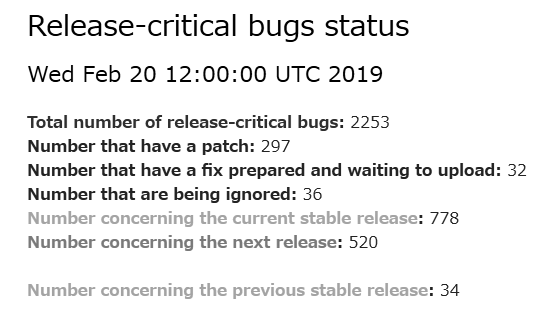
\includegraphics[width=0.45\hsize]{image201902/debian-rcbug-1_20190220_gray.png}
  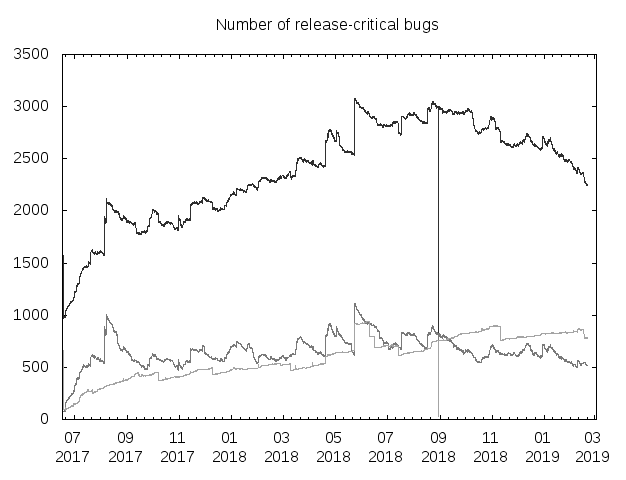
\includegraphics[width=0.45\hsize]{image201902/debian-rcbug-2_20190220_gray.png}
  % https://bugs.debian.org/release-critical/
\end{center}




\subsubsection{Debian 9 $B$+$i(B 10 $B$NJQ99E@(B}


$B!Z$4Cm0U$/$@$5$$![(B
$B$3$N;qNA$O(B2$B7n8=:_$N$b$N$G$9!#%j%j!<%9%N!<%H(B\footnote{\url{https://www.debian.org/releases/buster/amd64/release-notes/index.ja.html}}$B$r;2>H$7$F$/$@$5$$!#(B


usr-merge $B$N40A4E,MQ$O(B Buster $B$G$O0lIt8+Aw$j(B

\begin{itemize}
\item \url{https://wiki.debian.org/UsrMerge}
\item /bin,/sbin,/lib$B$r!"(B/usr/bin,/usr/sbin,/usr/lib $B$X$N%7%s%\%j%C%/$K$9$k$3$H(B
\item $B0lIt$N%Q%C%1!<%8$GLdBj$,=P$?$?$a!"5;=Q0Q0w2q$b4^$a$F(BBuster $B$G$O$I$&$9$k$+(B $B5DO@$K$J$C$?(B
  \begin{itemize}
  \item $B5DO@$N7k2L!"(Busr-merge $B$N<h$jAH$_$O(B Buster $B$N%j%j!<%98e$K2~$a$F?J$a$3$H$K$J$C$?(B
  \item $B!V(Btech-ctte: Should debootstrap disable merged /usr by default?$B!W(B \url{https://bugs.debian.org/cgi-bin/bugreport.cgi?bug=914897}
  \item $B!V(Busrmerge -- plan B?$B!W$N%9%l%C%I$r;2>H(B \url{https://lists.debian.org/debian-devel/2018/11/msg00354.html}
  \end{itemize}
\end{itemize}




%\begin{frame}{Debian 9 $B$+$i(B 10 $B$NJQ99E@(B}% [containsverbatim]
%
%secure boot
%  
%\begin{itemize}
%\item secure boot$BBP1~$GLdBj$H$J$k%P%0$O$9$Y$F2r7h:Q$_(B
%\item $B3'$5$s$,$*;}$A$N(BPC$B$G;n$7$?F0:n7k2L$NJs9p$rJg=8$7$F$$$^$9(B
%  \begin{itemize}
%  \item \url{https://wiki.debian.org/SecureBoot/Testing}
%  \end{itemize}
%\end{itemize}
%    
%



linux kernel$B$H(Bglibc$B$N%P!<%8%g%s%"%C%W$KH<$&JQ99(B
  
\begin{itemize}
\item apparmor$B$O%G%U%)%k%H$GM-8z$K$J$k(B
\item Buster$B$r%3%s%F%J4D6-$GF0$+$9>l9g$N@)8B(B
  \begin{itemize}
  \item glibc-2.26$B0J9_$r:NMQ$7$F$*$j!"(Blinux-3.2$B0J9_$,I,MW(B
  \item $B%[%9%HB&$,$H$F$b8E$$%5!<%P$N>l9g$K(B Buster $B$,%3%s%F%J4D6-$GF0$+$J$$>l9g$"$j(B
  \end{itemize}
\item Buster$B$r%[%9%H4D6-$GF0$+$9>l9g$N@)8B(B
  \begin{itemize}
  \item amd64$B$K$*$$$F!"8E$$(B'virtual syscall' $B$,%G%U%)%k%H$GL58z(B
  \item glibc-2.13$B0J2<$N%7%9%F%`$O%3%s%F%J4D6-$GF0$+$J$$(B
    \begin{itemize}
    \item Debian-7$B0J2<!"(BRHEL/CentOS-6 $B0J2<$,3:Ev(B
    \end{itemize}
  \item $BM-8z$K$9$k>l9g$O%+!<%M%k%Q%i%a!<%?$K(B vsyscall=emulate $B$rDI2C(B
  \end{itemize}
\end{itemize}





GNOME $B$O(B Wayland $B$G$NF0:n$,%G%U%)%k%H(B

\begin{itemize}
\item $B!V(BGNOME on Xorg$B!W$bA*$Y$^$9(B
\item $BB>$N%G%9%/%H%C%W4D6-$O(B Xorg $B$GF0:n$7$^$9(B
\item GNOME $B$G(B Wayland $B$r;H$&>l9g$KF|K\8l$rF~NO$G$-$J$$$3$H$,$"$k(B
  \begin{itemize}
  \item $BF|K\8lF~NO=hM}!J(BInput Method$B!K<~$j$KLdBj$,;D$C$F$*$j!"=$@5BP1~Cf(B
  \end{itemize}
\end{itemize}

\begin{center}
  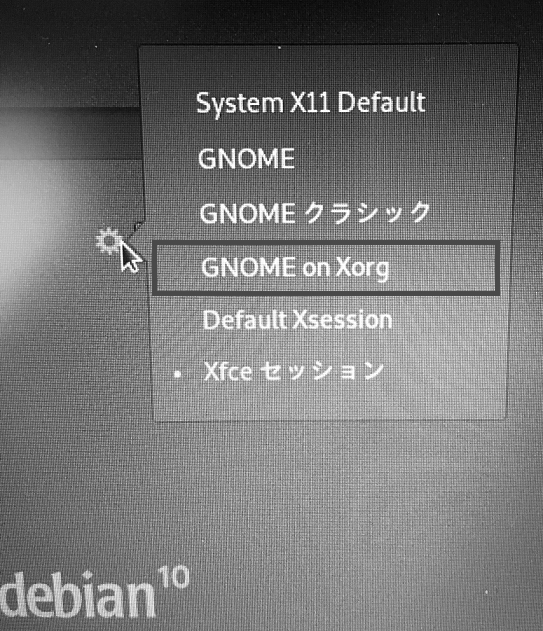
\includegraphics[width=0.5\hsize]{image201902/GDM_GNOME_select_mark_gray.png}
\end{center}





  \begin{itemize}
  \item openssl-1.1.1$B7O$N:NMQ$K$h$j(BTLSv1.3$B$,MxMQ2DG=(B
  \item openssh$B$K$*$$$F(BSSH 1$B%W%m%H%3%k$,40A4:o=|!#(BSSH 2$B%W%m%H%3%k$rMxMQ$9$k$3$H!#(B
  \item Debian 10$B$G$O!"(BDebian 9$B$HF1$8%"!<%-%F%/%A%c$r%5%]!<%H$9$k(B\footnote{2019$BG/(B2$B7n$NK\5-;v:n@.;~$K$O%5%]!<%H%"!<%-%F%/%A%c$O$^$@3NDj$7$F$$$J$+$C$?!#(B}
    \begin{itemize}
    % \item $B;29M!'(BDebian 9$B$G%5%]!<%H$7$F$$$k%"!<%-%F%/%A%c(B
    \item amd64, i386$B!J(Bi686$B0J9_!K(B, armel, armhf, arm64, mips, mipsel, mips64el, ppc64el, s390x
    \end{itemize}
  \end{itemize}




\subsubsection{$B%P%0%l%]!<%H(B}

  \begin{itemize}
  \item $B2?$+$*$+$7$$F0:n$dIT6q9g$r8+$D$1$?>l9g$O%P%0%l%]!<%H$r$*4j$$$7$^$9(B
  \item $B%P%0%l%]!<%H$N;EJ}!J%l%]!<%H$O1Q8l$GAw$kI,MW$"$j!K(B
    \begin{itemize}
    \item \url{https://www.debian.org/Bugs/Reporting.ja.html}
    \end{itemize}
  \item $B%P%0%l%]!<%H$NA0$K$A$g$C$HAjCL$7$F$_$?$$J}$O!"F|K\8l$N(BDebian JP$B%a!<%j%s%0%j%9%H$d!"(BSNS$B$GAjCL$7$F$_$F$/$@$5$$(B
    \begin{itemize}
    \item \url{https://www.debian.or.jp/community/ml/openml.html}
    \item Twitter: @debian\_jp
    \end{itemize}
  \end{itemize}


%-----------------------

\subsection{Debian Updates}

% $BH>G/4V$N0J2<(BML$B$+$iH4?h$7$F>R2p$9$k(B
%  debian-announce@lists.debian.org
%  debian-devel-announce@lists.debian.org

  %\begin{center}\Huge{Debian Updates}\end{center}



\subsubsection{released timeline}


\begin{itemize}
  \item 2018/11/10:  Updated Debian 9.6  released
  \item 2019/01/23:  Updated Debian 9.7  released
  \item 2019/02/16:  Updated Debian 9.8  released
\end{itemize}




\subsubsection{Bits from the DPL}


Bits from the DPL

\begin{itemize}
\item $B7n$K(B1$B2s(B"debian-devel-announce@lists.debian.org"$B$N(BML$B$K(BChris$B$5$s$,%W%m%8%'%/%H$N?JD=$rJs9p$7$F$$$k(B
\item $B;~4V$N$J$$J}$G$b$3$l$rFI$s$G$*$1$P(BDebian Project$B$NBg$^$+$JF0$-$,$o$+$k(B
\end{itemize}

\small{
\begin{itemize}

\item 2018/10/31 \url{https://lists.debian.org/debian-devel-announce/2018/10/msg00005.html}
\item 2018/11/30 \url{https://lists.debian.org/debian-devel-announce/2018/11/msg00007.html}
\item 2018/12/31 \url{https://lists.debian.org/debian-devel-announce/2018/12/msg00006.html}
\item 2019/01/31 \url{https://lists.debian.org/debian-devel-announce/2019/01/msg00010.html}

\end{itemize}
}




\subsubsection{Rust}


\begin{itemize}
\item 2018/11/02: Rust now available on 14 Debian architectures \\
\ \\
  \small{Rust$B%3%s%Q%$%i$N%V!<%H%9%H%i%C%W$,(Bmips$B!"(Bmips64el$B!"(Bmipsel$B!"(Bpowerpcspe$B$G$b$G$-$k$h$&$K$J$C$?!#(B\url{https://lists.debian.org/debian-devel-announce/2018/11/msg00000.html}}

\end{itemize}




\subsubsection{SSH restriction}


\begin{itemize}
\item 2018/11/10: incoming SSH restriction for *.debian.org \\
\ \\
  \small{debian.org$B$N%I%a%$%s$r;}$D0lIt$N%[%9%H$K$*$$$F!"%;%-%e%j%F%#$N4QE@$+$i(Bdebian.org$B$N%5!<%P$+$i$N$_(Bssh$B@\B3$r<u$1IU$1$k$h$&$K@_Dj$rJQ99$7$?!#(B\url{https://lists.debian.org/debian-devel-announce/2018/11/msg00003.html}}

\end{itemize}




\subsubsection{CTTE vendor-specific patch}


\begin{itemize}
\item 2018/11/13: CTTE decision on vendor-specific patch series (bug \#904302) \\
\ \\
  \small{DPKG$B$K$"$k%Y%s%@!<8GM-%Q%C%A5!G=!J<g$KGI@8%G%#%9%H%j%S%e!<%7%g%s$N(BUbuntu$B$J$I$,MxMQ$7$F$$$k!K$r7QB3MxMQ$9$k$+MxMQ$r;_$a$k$+5DO@$,$"$C$?!#5DO@$N7k2L!"(BDebian 10 Buster$B$N%j%j!<%98e$OMxMQ$r;_$a$k$Y$-$H$NDs0F$,$5$l$?!#(B\url{https://lists.debian.org/debian-devel-announce/2018/11/msg00004.html}}

\end{itemize}




\subsubsection{GSoC2019}


\begin{itemize}
\item 2019/01/16: Google Summer of Code 2019\\
\ \\
\small{Google Summer of Code 2019$B$G<h$jAH$`%W%m%8%'%/%H$N(Bwiki$B%Z!<%8$,N)$A>e$,$C$?!#1~Jg$NNc$O!"%W%m%8%'%/%H$NNc$O!V(BAndroid SDK Tools in Debian$B!W!"!V(BContinuous Integration for biological applications inside Debian$B!W!"!V(BDebian PHP Packaging$B!W!"!V(BNew Contributor Wizard$B!W!V(BReproducible Builds$B!W$J$I!#(B\url{https://lists.debian.org/debian-devel-announce/2019/01/msg00007.html}}

\end{itemize}




%-----------------------

\subsection{$BF|K\8l$K$h$k(BDebian$B$N>pJs(B}


\begin{itemize}
  \item Debian JP Project \\
      \url{https://www.debian.or.jp}
  \item $BEl5~%(%j%"(BDebian$BJY6/2q(B\\
      \url{https://tokyodebian-team.pages.debian.net/}
  \item $B4X@>(BDebian$BJY6/2q(B \\
      \url{https://wiki.debian.org/KansaiDebianMeeting}
  \item Twitter \\
      \url{@debian_jp}
  \item  $B;(;o(B Software Design $B5;=QI>O@<RH/9T(B \\
    $B!V(BDebian Hot Topics$B!W!"(BGPG$B4XO"$N5-;v$J$I!J3V7nO":\!K(B
\end{itemize}



%201903 tokyo
%-------------------------------------------------------------------------------
\dancersection{systemd$B$H(Bsysvinit$B$N%G!<%b%s$GF0:n$9$k(BDebian$B%Q%C%1!<%8$N:n$jJ}$rD4$Y$F$_$k(B}{$B?yK\!!E5=<(B}
%-------------------------------------------------------------------------------

\subsection{$B$O$8$a$K(B}

$B%G!<%b%s%W%m%0%i%`$r(Bdebian$B%Q%C%1!<%82=$9$k$K$O$I$N$h$&$K%Q%C%1!<%8$r:n@.$9$l$P$h$$$N$+M}2r$7$F$$$J$$$?$a!"D4$Y$F$_$^$7$?!#(B


\subsection{Debian$B$K$*$1$k(Binit$B$N;EAH$_(B}

$B0lHLE*$K(BUNIX/Linux$B7O$N(BOS$B$K$*$$$F%+!<%M%k$,:G=i$K8F$S=P$9!V(Binit$B!W$H$$$&%f!<%6%i%s%I%W%m%0%i%`(B\footnote{$B0lHLE*$K%W%m%;%9HV9f(B $B!V(B1$B!W$N>l9g$,B?$$$G$9!#(B}$B$,$"$j!"$3$N(Binit$B$,>oCs%W%m%0%i%`!J!a%G!<%b%s!K$N5/F0$dDd;_$r4IM}$7$^$9!#(B


Debian$B$K$*$1$k(Binit$B%7%9%F%`$N2r@b$O!"(BDebian $B%j%U%!%l%s%9$N!VBh(B3$B>O(B $B%7%9%F%`$N=i4|2=!W$K5-=R$,$"$j$^$9(B\footnote{\url{https://www.debian.org/doc/manuals/debian-reference/ch03.ja.html}}$B!#(B

Debian$B$G:NMQ$7$F$$$k(Binit$B%7%9%F%`$O!"@N$+$iB8:_$9$k!V(Bsysvinit$B!W!"?7@$Be$N!V(Bsystemd$B!W$,$"$j(B\footnote{$BB>$K$b(BOpenRC$B$H$$$&(Binit$B$b$"$j$^$9!#(B}$B!"(BDebian 8$B$+$i$O(Bsystemd$B$rI8=`$N(Binit$B%7%9%F%`$H$7$F:NMQ$7$F$$$^$9(B\footnote{systemd$B$,I8=`$J$N$O(BDebian GNU/Linux$B$N>l9g$G$9!#(Bsystemd$B$O(Blinux$B%+!<%M%k@lMQ$N%W%m%0%i%`$N$?$a!"(BkFreeBSD$B$d(BHurd$B$G$OF0$-$^$;$s!#(B}$B!#(B


Debian$B$G$O(Bsystemd$B$H(Bsysvinit$B$r@Z$jBX$($k$3$H$,$G$-$^$9(B\footnote{\url{https://wiki.debian.org/Init}}$B!#$=$N$?$a%G!<%b%s%W%m%0%i%`$N(Bdebian$B%Q%C%1!<%8$r:n$k$H$-$O!"(Bsystemd$B$H(Bsysvinit$B$N$I$A$i$N4D6-$G$b%G!<%b%s$r5/F0$G$-$k$h$&%Q%C%1!<%8$r:n$kI,MW$,$"$j$^$9!#(B


\subsection{Debian$B$K$*$1$k(Binit$B$,8F$S=P$95/F0!&Dd;_$N@_Dj%U%!%$%k(B}

\subsubsection{systemd: /lib/systemd/system/[package].service}

Debian$B$N(Bsystemd$B$,4IM}$9$k%G!<%b%s$N5/F0!&=*N;$O!"(B"systemctl" $B%3%^%s%I$G9T$$$^$9!#(B


systemctl$B%3%^%s%I$G4IM}$9$k%G!<%b%s$N@_Dj%U%!%$%k$O!"(B"/lib/systemd/system/[package].service" $B$KCV$$$F$$$^$9!#$3$N(B "[package].service" $B%U%!%$%k$K%W%m%0%i%`$N%U%!%$%k%Q%9$d4D6-@_Dj%U%!%$%k!"<B9T$9$k%3%^%s%I$r5-=R$7$^$9(B\footnote{service$B%U%!%$%k$N5-=RJ}K!$O!"(B\url{https://www.freedesktop.org/software/systemd/man/systemd.service.html} $B$r;2>H!#(B}$B!#(B


$BNc$H$7$F!"(Bnginx-full$B%Q%C%1!<%8$r8+$F$_$^$7$g$&!#(B


nginx$B$r5/F0$9$k>l9g$O0J2<$N%3%^%s%I$r<B9T$7$^$9!#(B

\begin{commandline}
# systemctl start nginx
\end{commandline}

nginx$B$rDd;_$9$k>l9g$O0J2<$N%3%^%s%I$r<B9T$7$^$9!#(B

\begin{commandline}
# systemctl stop nginx
\end{commandline}


$B>e5-$N(Bsystemctl$B%3%^%s%I$r<B9T$7$?$H$-!"0J2<$N(B"nginx.service"$B$K=>$C$F(Bnginx$B$N5/F0!&=*N;$r(Bsystemd$B$,9T$C$F$$$^$9!#(B


\begin{commandline}
$ cat /lib/systemd/system/nginx.service | grep -v "\#"

[Unit]
Description=A high performance web server and a reverse proxy server
Documentation=man:nginx(8)
After=network.target nss-lookup.target

[Service]
Type=forking
PIDFile=/run/nginx.pid
ExecStartPre=/usr/sbin/nginx -t -q -g 'daemon on; master_process on;'
ExecStart=/usr/sbin/nginx -g 'daemon on; master_process on;'
ExecReload=/usr/sbin/nginx -g 'daemon on; master_process on;' -s reload
ExecStop=-/sbin/start-stop-daemon --quiet --stop --retry QUIT/5 --pidfile /run/nginx.pid
TimeoutStopSec=5
KillMode=mixed

[Install]
WantedBy=multi-user.target  
\end{commandline}


\subsubsection{sysvinit: /etc/init.d/[package]}

Debian$B$N(Bsysvinit$B$,4IM}$9$k%G!<%b%s$N5/F0!&=*N;$O!"(B"service"$B%3%^%s%I$G9T$$$^$9(B\footnote{Debian GNU/Linux 8 $B0J9_$G$O(Bsystemd$B$,%G%U%)%k%H$N$?$a(B \url{https://wiki.debian.org/Init} $B$N<j=g$r9T$&$H(Bsysvinit$B$KJQ99$G$-$^$9!#(B}$B!#(B


service$B%3%^%s%I$G4IM}$9$k%G!<%b%s$N@_Dj%U%!%$%k$O!"(B"/etc/init.d/[package]"$B$KCV$$$F$$$^$9!#$3$N(B"[package]"$B%U%!%$%k$O%7%'%k%9%/%j%W%H$G$"$j!"%W%m%0%i%`$N%U%!%$%k%Q%9$d4D6-@_Dj%U%!%$%k!"<B9T$9$k%3%^%s%I$r5-=R$7$^$9!#(B


service$B%3%^%s%I$+$i8F$S=P$9%9%/%j%W%H$r:n@.$9$k$K$"$?$j!"0J2<$N%X%k%Q!<%9%/%j%W%H$,$"$j$^$9!#(B

\begin{itemize}
  \item /lib/init/vars.sh
  \item /lib/lsb/init-functions
  \item /sbin/start-stop-daemon
\end{itemize}


$BNc$H$7$F!"(Bnginx-full$B%Q%C%1!<%8$r8+$F$_$^$7$g$&!#(B


nginx$B$r5/F0$9$k>l9g$O0J2<$N%3%^%s%I$r<B9T$7$^$9!J(Bsystemctl$B$N>l9g$H%3%^%s%I$N=gHV$,0c$$$^$9!K!#(B

\begin{commandline}
# service nginx start
\end{commandline}

nginx$B$rDd;_$9$k>l9g$O0J2<$N%3%^%s%I$r<B9T$7$^$9!#(B

\begin{commandline}
# service nginx stop
\end{commandline}


$B>e5-$N(Bservice$B%3%^%s%I$r<B9T$7$?$H$-!"(Bnginx$B$N5/F0!&=*N;$r(B "/etc/init.d/nginx" $B$,9T$C$F$$$^$9!#(B

$B"(D9$$$?$a0lIt>JN,$7$F$$$^$9!#(B

\begin{commandline}
$ cat /etc/init.d/nginx

#!/bin/sh

### BEGIN INIT INFO
# Provides:       nginx
# Required-Start:    $local_fs $remote_fs $network $syslog $named
# Required-Stop:     $local_fs $remote_fs $network $syslog $named
# Default-Start:     2 3 4 5
# Default-Stop:      0 1 6
# Short-Description: starts the nginx web server
# Description:       starts nginx using start-stop-daemon
### END INIT INFO

PATH=/usr/local/sbin:/usr/local/bin:/sbin:/bin:/usr/sbin:/usr/bin
DAEMON=/usr/sbin/nginx
NAME=nginx
DESC=nginx

# Include nginx defaults if available
if [ -r /etc/default/nginx ]; then
        . /etc/default/nginx
fi

STOP_SCHEDULE=''${STOP_SCHEDULE:-QUIT/5/TERM/5/KILL/5}''

test -x $DAEMON || exit 0

. /lib/init/vars.sh
. /lib/lsb/init-functions

# Try to extract nginx pidfile
PID=$(cat /etc/nginx/nginx.conf | grep -Ev '^\s*#' | awk 'BEGIN { RS=''[;{}]'' } { if ($1 == ``pid'') print $2 }' | head -n1)
if [ -z ``$PID'' ]; then
    PID=/run/nginx.pid
fi

if [ -n ``$ULIMIT'' ]; then
    # Set ulimit if it is set in /etc/default/nginx
    ulimit $ULIMIT
fi

start_nginx() {
    # Start the daemon/service
    #
    # Returns:
    #   0 if daemon has been started
    #   1 if daemon was already running
    #   2 if daemon could not be started
    start-stop-daemon --start --quiet --pidfile $PID --exec $DAEMON --test > /dev/null \
        || return 1
    start-stop-daemon --start --quiet --pidfile $PID --exec $DAEMON -- \
        $DAEMON_OPTS 2>/dev/null \
        || return 2
}

  (snip)

stop_nginx() {
    # Stops the daemon/service
    #
    # Return
    #   0 if daemon has been stopped
    #   1 if daemon was already stopped
    #   2 if daemon could not be stopped
    #   other if a failure occurred
    start-stop-daemon --stop --quiet --retry=$STOP_SCHEDULE --pidfile $PID --name $NAME
    RETVAL=''$?''
    sleep 1
    return ``$RETVAL''
}

(snip)

case ``$1'' in
    start)
        log_daemon_msg ``Starting $DESC'' ``$NAME''
        start_nginx
        case ``$?'' in
            0|1) log_end_msg 0 ;;
            2)   log_end_msg 1 ;;
        esac
        ;;
    stop)
        log_daemon_msg ``Stopping $DESC'' ``$NAME''
        stop_nginx
        case ``$?'' in
            0|1) log_end_msg 0 ;;
            2)   log_end_msg 1 ;;
        esac
        ;;

(snip)

    *)
        echo ``Usage: $NAME {start|stop|restart|reload|force-reload|status|configtest|rotate|upgrade}'' >&2
        exit 3
        ;;
esac
\end{commandline}


\subsection{init$B@_Dj$r9T$&(Bdebian$B%Q%C%1!<%8:n@.J}K!(B}

\subsubsection{$BA0Ds(B}

Debian GNU/Linux 9 (stretch) $B$N4D6-$rA0Ds$H$7$^$9!#(B


debian$B%Q%C%1!<%8$r:n@.$9$k%D!<%k$O!"$[$H$s$I$N%Q%C%1!<%8$G(Bdebhelper$B$,;H$o$l$F$$$^$9(B\footnote{\url{https://www.debian.org/doc/manuals/packaging-tutorial/packaging-tutorial.ja.pdf} $B$N(B2019$BG/(B3$B7n(B4$BF|$N;qNA$K$*$$$F!!(Bdebhelper$B$N:NMQN($O(B98\%$B$H$N?t;z$,$"$j$^$9!#(B} $B!#:#2s$O!"(Bdebhelper$B$r;H$C$F%Q%C%1!<%8:n@.$r9T$&$3$H$rA0Ds$H$7$F@bL@$7$^$9!#(B


debian$B%Q%C%1!<%8$r:n@.$9$k$K$"$?$j!"4pK\E*$J;v9`$rCN$k%I%-%e%a%s%H$O0J2<$K$J$j$^$9$N$GFI$s$G$_$F$/$@$5$$!#(B

\begin{itemize}
\item \url{https://wiki.debian.org/ja/Packaging}
\item packaging-tutorial$B%Q%C%1!<%8$N(BPDF$B%U%!%$%k(B \\/usr/share/doc/packaging-tutorial/packaging-tutorial.ja.pdf\footnote{web$BHG$O$3$A$i!#(B \url{https://www.debian.org/doc/manuals/packaging-tutorial/packaging-tutorial.ja.pdf}}
\item Debian $B?7%a%s%F%J!<%,%$%I(B \\\url{https://www.debian.org/doc/manuals/maint-guide/index.ja.html}
\item Debian Policy Manual \\\url{https://www.debian.org/doc/debian-policy/}
\end{itemize}  


debhelper$B$G(Bdebian$B%Q%C%1!<%8$N:n@.$r9T$&>l9g$O0J2<$N%Q%C%1!<%8$r%$%s%9%H!<%k$7$F$*$/$H$h$$$G$7$g$&(B\footnote{$B@N$O(Bsystemd$B$KBP1~$9$k>l9g$K$O(Bdh-systemd$B%Q%C%1!<%8$,I,MW$G$7$?$,!"(Bstretch$B$G$O(Bdebhelper$B$KE}9g$5$l$F$$$k$?$a%$%s%9%H!<%kITMW$G$9!#(B}$B!#(B


\begin{commandline}
# apt-get update
# apt-get install build-essential dpkg-dev devscripts debhelper dh-make quilt
\end{commandline}


\subsubsection{systemd$B$KBP1~$9$k@_Dj(B}

$B0J2<$N(Bweb$B%Z!<%8$K2r@b%I%-%e%a%s%H$,$"$j$^$9$N$G!"$3$l$r2r@b$7$F$$$-$^$9!#(B

\begin{itemize}
\item \url{https://wiki.debian.org/Teams/pkg-systemd/Packaging}
\end{itemize}


systemd$B$N@_Dj$r9T$&$K$ODL>o$N%Q%C%1!<%8:n@.:n6H$N$[$+!"0J2<$rDI2C$G:n6H$9$kI,MW$,$"$j$^$9!#(B

\begin{itemize}
\item debian/rules$B$N=$@5(B
\item debian/control$B$N=$@5(B
\item \bf{"debian/package.service"} $B$N:n@.(B
\end{itemize}


\subsubsubsection{debian/rules$B$N=$@5(B}

debian/rules$B%U%!%$%k$O!"(Bdh\_make$B%3%^%s%I$r<B9T$7$?$H$-$K$R$J7A%U%!%$%k$,:n@.$5$l$^$9!#(B


systemd$B$G4IM}$9$k%G!<%b%s$N>l9g$O!"0J2<$N$h$&$K(B "--with systemd" $B$NDj5A$rDI2C$7$^$9!#$3$N(B "--with" $B%*%W%7%g%s$O(B debhelper $B$N(B addon $B$N=hM}$r<B9T$9$k$h$&$K;XDj$9$k$b$N$G$9(B\footnote{man dh(1) $B$r;2>H!#(B}$B!#(B

\begin{commandline}
%:
    dh $@ --with systemd
\end{commandline}


$B$3$N(B "--with systemd" $B$N(B addon $B;XDj$,$"$k>l9g$O(B debian $B%Q%C%1!<%8$N%S%k%I=hM}$G(B "dh\_systemd\_enable"$B!"(B "dh\_systemd\_start" $B$r<B9T$9$k$h$&$K$J$j$^$9!#(B


"dh\_systemd\_enable" $B$O!"(B"\# systemctl \{enable/disable\} package" $B$r<B9T$9$k$h$&;XDj$9$k$b$N$G!"<!2s$N(BOS$B5/F0;~$K<+F0$G(B package $B$N%G!<%b%s$r5/F0$9$k$+;XDj$G$-$^$9!#(B


"dh\_systemd\_start" $B$O!"(B"\# systemctl \{start/stop/restart\} package" $B$r<B9T$9$k$h$&;XDj$9$k%3%^%s%I$G!"%Q%C%1!<%8$N%$%s%9%H!<%k=hM}$G%G!<%b%s$r5/F0$9$k$+!":F5/F0$9$k$+$J$I$r;XDj$G$-$^$9!#(B


\subsubsubsection{debian/control$B$N=$@5(B}

"debian/control"$B%U%!%$%k$O!"(Bdh\_make$B%3%^%s%I$r<B9T$7$?$H$-$K$R$J7A%U%!%$%k$,:n@.$5$l$^$9!#(B


"debian/control" $B%U%!%$%k$r=q$/>e$G!"(Bdebhelper$B$N8_49@-%l%Y%k$r5-=R$9$k(B"debian/compat" $B%U%!%$%k$,$"$j$^$9!#$3$N(B"debian/compat"$B%U%!%$%k$NCf?H$,(B"10"$B0J>e$G$"$l$P(B "debian/control" $B%U%!%$%k$r<!$N$h$&$K=q$-$^$9!#(B

\begin{commandline}
Build-Depends: debhelper (>= 9.20160709)
\end{commandline}

$B$b$7!"(B"debian/compat" $B$NCf?H$,(B "10" $BL$K~$G$"$l$P(B systemd $B8~$1$N=hM}$OJLES(B dh-systemd $B%Q%C%1!<%8$,I,MW$J$?$a(B\footnote{Debian 8 jessie $B8~$1$N%Q%C%1!<%8$r:n@.$9$k>l9g$,3:Ev$7$^$9!#(B}$B!"<!$N$h$&$K=q$-$^$9!#(B

\begin{commandline}
Build-Depends: debhelper (>= 9.20150101), dh-systemd (>= 1.5)
\end{commandline}


\subsubsubsection{debian/package.service $B$N:n@.(B}


"package.service" $B%U%!%$%k$O!"(Bdh\_make$B%3%^%s%I$r<B9T$7$?$H$-$K$R$J7A%U%!%$%k$,:n@.$5$l$^$;$s!#(B

$B$=$N$?$a!"B>$N%Q%C%1!<%8$N(B "package.service" $B%U%!%$%k$r;29M$K$7$D$D!"(Bservice$B%U%!%$%k$N%^%K%e%"%k$r$_$F:n@.$7$F$/$@$5$$(B\footnote{\url{https://www.freedesktop.org/software/systemd/man/systemd.service.html}}

"package.service" $B%U%!%$%k$r:n@.$7$F$*$/$H!"(Bdebian $B%Q%C%1!<%8$N%S%k%I=hM}Cf$N(B "dh\_installinit" $B$N=hM}$G(B "package.service" $B%U%!%$%k$r(B "/lib/systemd/system" $BG[2<$X%$%s%9%H!<%k$9$k$h$&=hM}$7$^$9!#(B


\subsubsection{sysvinit$B$KBP1~$9$k@_Dj(B}


sysvinit$B$N@_Dj$r9T$&$K$O!"DL>o$N%Q%C%1!<%8:n@.:n6H$N$[$+!"0J2<$rDI2C$G:n6H$9$kI,MW$,$"$j$^$9!#(B

\begin{itemize}
\item \bf{"debian/package.init"} $B$N:n@.(B
\end{itemize}


\subsubsubsection{debian/package.init $B$N:n@.(B}


"packages.init" $B%U%!%$%k$O!"(Bdh\_make$B%3%^%s%I$r<B9T$7$?$H$-$K$R$J7A%U%!%$%k$,:n@.$5$l$^$;$s(B\footnote{$B2a5n$K$O(Bdh\_make$B%3%^%s%I$G(B"debian/init.d.ex" $B$H$$$&$R$J7A%U%!%$%k$,:n@.$5$l$?$N$G$9$,!"(BDebian 8$B$K$*$1$k(Bsystemd$B$X$N0\9T$N2aDx$G:n@.$5$l$J$/$J$j$^$7$?!#(B}$B!#(B


$BB>$N%Q%C%1!<%8$N(Binit$B%U%!%$%k$r;29M$K$9$k$+!"8E$$%P!<%8%g%s$N(Bdebhelper$B$K4^$^$l$k(B"init.d.ex" $B%U%!%$%k$r<hF@$7$F:n@.$7$F$/$@$5$$(B\footnote{\url{https://sources.debian.org/data/main/d/dh-make/1.20140617/lib/debian/init.d.ex}}$B!#(B


"package.init" $B%U%!%$%k$r:n@.$7$F$*$/$H!"(Bdebian$B%Q%C%1!<%8$N%S%k%I=hM}Cf$N(B "dh\_installinit"$B$N=hM}$G(B "package.init" $B%U%!%$%k$r(B "/etc/init.d" $BG[2<$X%$%s%9%H!<%k$9$k$h$&=hM}$7$^$9!#(B


\subsection{$B$^$H$a(B}

Debian$B$K$*$1$k(Binit$B$N@bL@$H%G!<%b%s$N5/F0!&=*N;$r9T$&(Bdebian$B%Q%C%1!<%8$r(Bdebhelper$B$G$I$&:n$k$+@bL@$7$^$7$?!#(Bdebian/[package].service $B%U%!%$%k!"(Bdebian/[package].init $B%U%!%$%k$NB8:_$r3P$($F$*$/$H$h$$$H;W$$$^$9!#(B


debhelper$B$r;H$C$?(Bdebian$B%Q%C%1!<%8$N%S%k%I$G$O(B  dh\_installinit $B$N=hM}$G(B systemd/sysvinit $B$N@_Dj%U%!%$%k$r%Q%C%1!<%8$KG[CV$7$F$$$^$9!#(B


$B$^$?!"#1$D$N%=!<%9%Q%C%1!<%8$+$iJ#?t$N%P%$%J%j%Q%C%1!<%8$r:n$k>l9g$K%U%!%$%kL>$NL?L>5,B'$,0[$J$k$J$I0c$$$b=P$F$-$^$9!#$=$l$i$K$D$$$F$OB>$N%Q%C%1!<%8$r;29M$K$7$F3P$($F$$$/$H$h$$$H;W$$$^$9!#(B


\subsection{$B;29MJ88%(B}

\begin{itemize}
\item $B!V(BTeams pkg-systemd Packaging$B!W(B \url{https://wiki.debian.org/Teams/pkg-systemd/Packaging}
\item mkouhei (2014) $B!V(BHow to create a Debian package of support to sysvinit, upstart, systemd$B!W(B \url{https://d.palmtb.net/2014/01/30/how_to_create_a_debian_package_of_support_to_sysvinit__upstart__systemd.html}
\item @henrich (2016) $B!V(Bdh-systemd$B$O(Bdebhelper 9.20160709$B$GE}9g$5$l$?!W(B \url{https://qiita.com/henrich/items/e1651e3284c6b3d0d39e}
\end{itemize}

\dancersection{\mbox{Rust$B$G=q$$$?%D!<%k$N(B}\mbox{debian$B%Q%C%1!<%8%s%0$K(B}\mbox{$BD)@o$7$F$_$?OC(B($B2>(B)}}{$B>.NS(B $B9n4u(B}

\subsection{$B$O$8$a$K(B}

$B:#2s$NFbMF$G$9$,!":G6a8D?ME*$K?($j$@$7$?(BRust$B$H$$$&%W%m%0%i%_%s%08@8l$K$D$$$F!"(B
$B$=$b$=$b$I$&$$$&8@8l$J$s$@$H$$$&$4>R2p(B($B$H$$$C$F$b!";d$bJY6/Cf$N?H$G$9$,(B)$B$H!"(B
Rust$B$G=q$$$?%D!<%k$N(Bdeb$B$r:n$C$F$_$k!"$H$$$&$H$3$m$^$G$rL\I8$H$7$F$$$^$9!#(B

\subsection{Rust$B$H$O(B}

Rust$B$H$O!"(BMozilla$B$,%V%i%&%6%(%s%8%s(BServo$B$N$?$a$K3+H/$7$?%7%9%F%`%W%m%0%i%_%s%08@8l$G$9!#(B
2018$BG/$N%9%?%C%/%*!<%P!<%U%m!<$ND4::(B%
\footnote{\url{https://insights.stackoverflow.com/survey/2018}}%
$B$G0&$5$l$F$$$k8@8l%i%s%-%s%0(B1$B0L$K$J$k$J$I!"(B
$B:G6a$G$O7k9=%a%8%c!<$K$J$C$F$$$F$$$k46$8$N8@8l$G$9!#(B
$BFCD'$H$7$F$O!"0BA4@-!&JB9T@-$K$D$$$F9M$($i$l$F@_7W$5$l$F$$$kE@$G!"(B
$B$+$D!"$_$s$JBg9%$-(B(?)$B@EE*7?IU$18@8l$G$9!#(B

$B$J$*!"(BRust$B%W%m%0%i%^!<$N;v$r(Brustacean($B%i%9%H%7%"%s(B)$B$H$$$&$h$&$G$9!#(B
$B$3$l$O!"(B``Crustacean($B9C3LN`(B)`` $B$+$iMh$F$$$k$i$7$/!"(B
$B$=$N$;$$$+!"%*%i%$%j!<K\$NI=;f$O%*%*%R%m%P%*%&%.%,%K$H$$$&%+%K$G$9$7!"(B
$BHs8x<0%^%9%3%C%H$b$+$o$$$i$7$$%+%K(B($BL>A0$O(BFerris%
\footnote{\url{http://rustacean.net/}}%
)$B$K$J$C$F$^$9!#(B

\subsubsection{Rust$B$N%D!<%k%A%'!<%s$r%$%s%9%H!<%k(B}

$B$G$O$5$C$=$/(BRust$B$N%D!<%k%A%'!<%s$r%$%s%9%H!<%k$7$F$_$^$7$g$&!#(B
$B$5$F!"$b$A$m$s(BRust$B$N%D!<%k%A%'!<%s$N(Bdebian$B%Q%C%1!<%8$O$"$j$^$9$7!"(B
$B%m!<%+%k%^%7%s$K%$%s%9%H!<%k$;$:$K%V%i%&%6$G?'!9;n$;$k%5%$%H(B%
\footnote{\url{https://play.rust-lang.org/}}
$B$b$"$k$N$G$9$,!"(BRust$B$O(B2018$BG/$NG/Kv$K(B2018 Edition%
\footnote{\url{https://blog.rust-lang.org/2018/12/06/Rust-1.31-and-rust-2018.html}}%
$B$H$$$&Bg$-$a$J2~HG$,$"$C$?$N$G!"(B
$B$R$H$^$:(BRust$B8x<0$N<jCJ$G%D!<%k%A%'!<%s$r%$%s%9%H!<%k$7$^$7$g$&!#(B
$BNc$K$h$C$FNc$N$4$H$/!"3'MM$NBg;v$J%[!<%`%G%#%l%/%H%j$K?'!9$HF~$l$F$7$^$$$^$9$,!"(B
$B%P!<%8%g%s%"%C%W$NIQEY$O$=$l$J$j$K$"$k$N$G!"(BRust$B$N:G?7$rDI$C$F$$$/$J$i!"(B
$BL5M}$;$:$K8x<0$N%D!<%k%A%'!<%s$rF~$l$F$7$^$C$?J}$,L5Fq$+$H;W$$$^$9!#(B

Rust$B$N%D!<%k%A%'!<%s$G$9$,!"0JA0$O$=$&$G$b$J$+$C$?$_$?$$$G$9$,!":G6a$G$O(Brustup%
\footnote{\url{https://rustup.rs/}}%
$B$H$$$&%$%s%9%H!<%i!<$r;H$&$N$,8x<0<j=g$N$h$&$G$9!#(B
$B$$$+$K$b:G6a$N%D!<%k$C$]$$$G$9$,!"0J2<$N$h$&$K(Bcurl$B%3%^%s%I$rC!$$$F%$%s%9%H!<%k$7$^$9!#(B

\begin{commandline}
% curl https://sh.rustup.rs -sSf | sh
\end{commandline}

rustup$B$r;H$&$H!"%P%$%J%j$O(B \verb|~/.cargo| $B0J2<$K%$%s%9%H!<%k$5$l$^$9!#(B
$B%Q%9$rDL$7$?$$>l9g!"(B \verb|~/.cargo/env| $B$H$$$&%U%!%$%k$,$"$k$N$G!"(B
$B$=$A$i$r(B \texttt{source} $B$7$F$"$2$k$H$h$m$7$$$+$H;W$$$^$9!#(B
$B$R$H$^$:!"(B \texttt{cargo} $B$H$$$&%3%^%s%I$,;H$($k$h$&$K$J$C$F$$$?$iBg>fIW$G$9!#(B
$B$J$*!"!V$I$&$7$F$b(Bdeb$B$G!W$H$$$&J}$O(B \texttt{cargo} $B%Q%C%1!<%8$r%$%s%9%H!<%k$7$F$/$@$5$$!#(B
$B$=$N:]!"(B\texttt{rustc}$B$N%P!<%8%g%s$,(B2018 Edition$B$G$"$k(B1.31$B0J9_$G$"$k;v$,K>$^$7$$$G$9!#(B

\subsubsection{Hello World$B$7$F$_$k(B}

$B$G$O!"(Bcargo$B$,;H$($k$h$&$K$J$C$?$H$3$m$G!"(BHello World$B$7$F$_$^$7$g$&!#(B
Rust$B$N%W%m%8%'%/%H$O!"(B \verb|cargo new| $B$G:n@.$9$k$3$H$,$G$-$^$9!#(B
$B@N$O(B\verb|--bin|$B$r$D$1$J$$$H%i%$%V%i%jMQ$N%W%m%8%'%/%H$K$J$C$F$^$7$?$,!"(B
$B:G6a$N(Bcargo$B$G$"$l$P%G%U%)%k%H$,%P%$%J%jMQ$N%W%m%8%'%/%H$K$J$j$^$9!#(B
$B$=$l$G$O<B9T$7$F$_$^$7$g$&!#(B

\begin{commandline}
% cargo new hello
     Created binary (application) `hello` package
% tree
.
$B('(!(!(B Cargo.toml
$B(&(!(!(B src
    $B(&(!(!(B main.rs

1 directory, 2 files
\end{commandline}

$B<B9T$9$k$H!"$3$s$J46$8$K(BCargo.toml$B$H$$$&%U%!%$%k$H!"(B
main.rs$B$H$$$&%=!<%9%U%!%$%k$,:n@.$5$l$^$9!#(B
$B$=$&!"(BRust$B$N%=!<%9%U%!%$%k$N3HD%;R$O(B.rs$B$G$9!#(B
$B$=$N$?$a!"(BRust$B$N%W%m%8%'%/%H$N%&%'%V%5%$%H$O!"(B.rs$B%I%a%$%s$G:n$i$l$F$k;v$,$*$*$$$G$9!#(B
$B$A$J$_$K!"(B.rs$B$O%;%k%S%"$N%I%a%$%s$G$9!#(B

$B<B$O!"$3$N;~E@$G(BHello World$B$NH>J,$,40N;$7$F$$$^$9!#(B
src/main.rs$B$NCf?H$r8+$F$_$^$7$g$&!#(B

\begin{commandline}
fn main() {
    println!("Hello, world!");
}
\end{commandline}

$B$J$s$H!"4{$K(BHello World$B$N%3!<%I$,@8@.$5$l$F$$$^$9!#(B
$B$J$*!">\:Y$O>J$-$^$9$,!"(B \verb|println!()| $B$O4X?t$K8+$($^$9$,!"(B
$B%S%C%/%j%^!<%/$,IU$$$F$$$kJ*$O!"(BRust$B$G$O%^%/%m$G$"$C$?$j$7$^$9!#(B
$B$^$!!"?<$/IU$-2q$&A0$O!"FC$K5$$K$7$J$/$FNI$$$+$H;W$$$^$9!#(B
$B%S%k%I$7$F<B9T$9$k$K$O(B \verb|cargo run| $B$9$l$P(BOK$B$G$9!#(B

\begin{commandline}
% cargo run
   Compiling hello v0.1.0 (/path/to/hello)
    Finished dev [unoptimized + debuginfo] target(s) in 0.31s
     Running `target/debug/hello`
Hello, world!
\end{commandline}

\subsection{Rust$B$N9=J8Ey$N>R2p(B}

$B$=$l$G$O!"$3$3$+$i$O4JC1$K(BRust$B$N9=J8Ey$N>R2p$r$7$F$$$-$?$$$H;W$$$^$9!#(B
$B$J$*!";d$bJY6/Cf$N?H$G$9$N$G!"HyL/$K13$r=q$$$F$$$?$i$9$$$^$;$s!#(B
$B@53N$J;v$O!"(BThe Book%
\footnote{\url{https://doc.rust-lang.org/book/}}%
$B$H8F$P$l$k5$9g$NF~$C$?%I%-%e%a%s%H$,$"$j$^$9$N$G$=$A$i$r;29M$K$7$F$$$?$@$1$?$i$H;W$$$^$9!#(B

$B$J$*!"(BRust$B$OHf3SE*3X=,$,Fq$7$$$H$+8@$o$l$F$^$9$,!"(B
$B$J$s$GFq$7$$$N$+$K$D$$$F!"8D?ME*$K$O%*%i%$%j!<$N(BRust$BK\$G0zMQ$5$l$F$k(BQuora$B$K=q$+$l$?%3%a%s%H(B%
\footnote{\url{https://www.quora.com/What-do-C-C++-systems-programmers-think-of-Rust/answer/Mitchell-Nordine}}%
$B$,$7$C$/$jMh$?$N$G0zMQ$7$F$*$-$^$9!#(B
\begin{quotation}
I've found that Rust has forced me to learn many of the things that I was slowly learning as
``good practise'' in C/C++ before I could even compile my code.
\end{quotation}
$B;d$O:G6a2q<R$N;E;v$N4X78$G(BC++$B$NJY6/$b$9$k%O%a$K$J$C$F$k$N$G$9$,!"$^$5$K>e5-$HF1$846A[$G$9!#(B
$B$J$K$+!"(BC++$B$,$3$J$l$FMh$F!"(BC++11$B$"$?$j$G$h$&$d$/NI$$46$8$K$J$C$?5!G=$@$1$r<h$jF~$l$F$$$C$?$N$,(B
Rust$B$J$s$8$c$J$$$+$J$!$H!#(B

\subsubsection{$BJQ?t@k8@(B}

$BJQ?t$N@k8@$O(B\texttt{let}$B%-!<%o!<%I$r;H$$$^$9!#(B
$B7?$O!":G6a$N8@8l$C$]$/%3%m%s$N8e$K=q$-$^$9$,!"7?$,?dO@$G$-$k$J$i>JN,2DG=$G$9!#(B
$B$^$?!"%7%c%I!<%$%s%0$9$k$3$H$b2DG=$G!";XDj$,$J$1$l$P(Bimmutable$B$JJQ?t$K$J$k$N$G!"(B
mutable$B$JJQ?t$r:n$k>l9g$O(B\texttt{mut}$B%-!<%o!<%I$r;H$$$^$9!#(B
$B6qBNE*$JNc$r0J2<$K<($7$^$9!#(B

\begin{commandline}
fn main() {
    let x = 1;
    println!("x = {}", x);
    let x = 1.25;
    println!("x = {}", x);
    x = 1;   // $B%(%i!<$K$J$k(B($B$=$b$=$b(Bimmutable$B$@$1$I(B): expected floating-point number, found integer
    x = 1.5; // $B%(%i!<$K$J$k(B: cannot assign twice to immutable variable

    let mut y: u32 = 1;
    y -= 1;
    y -= 1;
    println!("y = {}", y);
}
\end{commandline}

$BNc$N(B2$B$DL\$N(B\verb|y -= 1;|$B$G$9$,!"%G%P%C%0%S%k%I$@$H%*!<%P!<%U%m!<$r8!CN$7$F<B9T;~$K%Q%K%C%/$r5/$3$7$^$9!#(B
$B%j%j!<%9%S%k%I(B(\verb|--release|$B%*%W%7%g%sIU$-$G(B\texttt{cargo}$B$r<B9T(B)$B$@$H(B
$B%Q%K%C%/$OH/@8$7$^$;$s$,!"$b$A$m$s$*$+$7$JCM$,I=<($5$l$^$9!#(B

$B$J$*!"4pK\E*$J7?$O0J2<$N$h$&$J$b$N$,$"$j$^$9!#(B

\begin{quote}
\begin{description}
 \item[$B@0?t(B]
	    \textbf{$BId9fL5$7(B:} \texttt{u8}, \texttt{u16}, \texttt{u32}, \texttt{u64}, \texttt{usize}\\
	    \textbf{$BId9fIU$-(B:} \texttt{i8}, \texttt{i16}, \texttt{i32}, \texttt{i64}, \texttt{isize}
 \item[$BIbF0>.?tE@(B] \textbf{$BC1@:EY(B:} \texttt{f32}$B!"(B\textbf{$BG\@:EY(B:} \texttt{f64}
 \item[$B%V!<%k(B] \texttt{bool}
 \item[$BJ8;z(B] \texttt{char}  (Unicode$B$N(B1$BJ8;z(B)
 \item[$BJ8;zNs(B] \texttt{String}
	    \begin{itemize}
	     \item $B$?$@$7!"J8;zNs%j%F%i%k$N(B \texttt{str} $B$,$"$C$F$H$F$b$d$d$3$7$$(B
	    \end{itemize}
 \item[$BG[Ns(B] \texttt{[T; N]} (\texttt{T}: $B7?(B,  \texttt{N}: $BMWAG?t(B)
 \item[$B%Y%/%?!<(B] \texttt{Vec<T>} (\texttt{T}: $B7?(B)
 \item[$B%9%i%$%9(B] \texttt{\&[T]} (\texttt{T}: $B7?(B)
\end{description}
\end{quote}

\texttt{String}$B$H(B\texttt{str}$B$,>/!9$d$d$3$7$$$G$9$,!"(B
$B%$%a!<%8$H$7$F$O(BC++$B$N(B\texttt{std::string}$B$H(B\texttt{char}$B$N4X78$K6a$$$h$&$J46$8$G$9!#(B
\texttt{String}$B$NJ}$O2DJQD9$G!"%a%b%j>e$N%$%a!<%8$r?^$K$9$k$H?^(B\ref{fig:str-string}$B$N$h$&$J46$8$G$9!#(B
\texttt{\&}$B$,$D$$$F$k(B\texttt{str}$B$O!"$3$N8e=R$9$k;2>H$K$J$C$F$^$9!#(B
$B$R$H$^$:!"0J2<$,$A$g$C$H$7$?%5%s%W%k%3!<%I$G$9!#(B

\begin{figure}[htbp]
 \begin{center}
  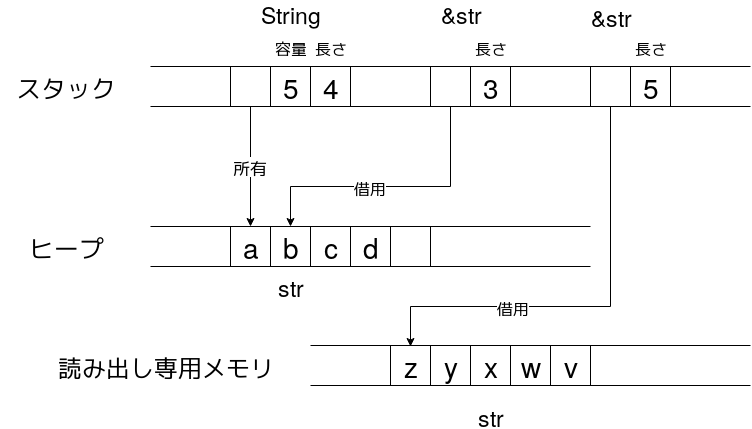
\includegraphics[keepaspectratio,height=4cm]{./image201903/rustlang-str-string.png}
  \label{fig:str-string}
  \caption{Rust$B$K$*$1$k(BString$B$H(Bstr$B$N0c$$(B}
 \end{center}
\end{figure}

\begin{commandline}
fn main() {
    let a = "abcd".to_string(); // String::from("abcd"); $B$G$b2D(B
    let b = &a[1..];
    let c = "zyxwv";

    let mut a = "abcd".to_string();
    //  ^^^  a$B$r(Bmutable$B$JJQ?t$H$7$F@k8@(B
    a.push_str("efg");  // OK

    let mut c = "zyxwv";

    // $B%(%i!<(B!: no method named `push_str` found for type `&str` in the current scope
    c.push_str("ut");  // str$B$K$ODI2C$G$-$J$$$N$G(Bpush_str$B%a%=%C%I$O$J$$(B
}
\end{commandline}

\subsubsection{$B4X?tDj5A(B}

$B$G$O!"4X?t$rDj5A$7$F$_$^$7$g$&!#(B
Rust$B$G$N4X?tDj5A$O!"(B\texttt{fn}$B%-!<%o!<%I$H(B`\texttt{->}'$B%H!<%/%s$r;H$$$^$9!#(B
$B$^$:$O!"C1=c$KB-$7;;$r9T$&4X?t(B\texttt{add}$B$rDj5A$7$F$_$^$9!#(B

\begin{commandline}
fn add(a: i32, b: i32) -> i32 {
    return a + b;
}

fn main() {
    println!("{}", add(1, 2));
}
\end{commandline}

$B$3$l$r(B\texttt{cargo}$B$G<B9T$9$k$H!"(B
($B6C$/$h$&$J;v$O0l@Z$J$$$G$9$,(B)$B0J2<$N$h$&$J7k2L$K$J$j$^$9!#(B

\begin{commandline}
% cargo run
Compiling function v0.1.0 (/path/to/examples/function)
Finished dev [unoptimized + debuginfo] target(s) in 0.20s
Running `target/debug/function`
3
\end{commandline}

$B$J$*!"$3$3$G$O(B\texttt{return}$B$r;H$$$^$7$?$,!"(B
Rust$B$G$O%;%_%3%m%s$rH4$+$9$HCM$r:n$k$?$a!"(B
$B%;%_%3%m%s$rH4$+$7$F=q$$$?0J2<$N$h$&$J(B\texttt{add}$B4X?t$b(B
$B>e5-$GDj5A$7$?4X?t$HF1$8F0:n$r$7$^$9(B($B%;%_%3%m%s$r=q$/$H%(%i!<$K$J$j$^$9(B)$B!#(B

\begin{commandline}
fn add(a: i32, b: i32) -> i32 {
    a + b
}
\end{commandline}

\subsubsection{$B=jM-8"(B}

$B$5$F!"$3$3$+$i0l5$$K(BRust$B$C$]$$OC$K$J$j$^$9!#(B
Rust$B$G$O!"%a%b%j$N0BA4@-$,9M$($i$l$F$$$k$H=q$-$^$7$?$,!"(B
$B$=$N$?$a$K=jM-8"(B($B1Q8l$G$O(Bownership)$B$H$$$&35G0$r;H$C$F$$$^$9!#(B
C++$B$G$b$"$k35G0$G$9$,!"$?$H$($P0J2<$N$h$&$J%W%m%0%i%`$,$"$C$?$H$7$^$9!#(B

\begin{commandline}
fn main() {
    let i0 = 1;
    let i1 = i0;
    let i2 = i0;

    let s0: String = "hoge".to_string();
    let s1 = s0;
    let s2 = s0;
}
\end{commandline}

$B$5$F!"$I$&$J$k$H;W$&$G$7$g$&$+(B?
$B@52r$O!"0J2<$N$h$&$K(B\texttt{s2}$B$K(B\texttt{s0}$B$rBeF~$7$F$$$k$H$3$m$G%(%i!<$K$J$j$^$9!#(B

\begin{commandline}
error[E0382]: use of moved value: `s0`
 --> ownership/src/main.rs:8:15
  |
6 |     let s0: String = "hoge".to_string();
  |         -- move occurs because `s0` has type `std::string::String`, which does not implement the `Copy` trait
7 |     let s1 = s0;
  |              -- value moved here
8 |     let s2 = s0;
  |              ^^ value used here after move
\end{commandline}

Rust$B$G$O!"BeF~!"4X?t$N0z?t!"4X?t$NLa$jCM$J$I$GCM$N=jM-8"$,0\F0$9$k$?$a!"(B
$B0lEY=jM-8"$r0\>y$7$F$7$^$C$?$i!"0\>y85$NJQ?t$O$=$N8e%"%/%;%9$G$-$J$/$J$j$^$9(B($B%3%s%Q%$%k;~$KE\$i$l$k(B)$B!#(B
$B$H$3$m$,!">e5-$N%3!<%I$G$O@0?t$NJ}$O%(%i!<$K$J$j$^$;$s!#(B
$B$3$l$O2?8N$+$H$$$&$H!"@0?t$J$I0lIt$N7?(B($B%5%$%:$,8GDj$G>.$5$$$b$N$,<g(B?)$B$O0\F0$;$:$K%3%T!<$K$J$j$^$9!#(B
$B<B$O%(%i!<%a%C%;!<%8$K$"$k(BCopy trait$B$H$$$&$N$,%_%=$G!"(B
$B@0?t7?$O$3$N(BCopy trait$B$r<BAu$7$F$$$k$+$i$=$&$$$C$?F0:n$K$J$C$F$$$^$9!#(B
trait$B$K$D$$$F$O8e=R$7$^$9!#(B

$B4X?t$N0z?t$G$b=jM-8"$O0\F0$9$k$N$G!"0J2<$N$h$&$J%3!<%I$b%"%&%H$G$9!#(B

\begin{commandline}
fn consume(_s: String) {}

fn main() {
    let h: String = "Hello World".to_string();
    consume(h);
    let hh = h;
}
\end{commandline}

$B%S%k%I$9$k$H!"4X?t(B\texttt{consume}$B%3!<%k;~$K(B\texttt{h}$B$,0\F0$7$F$7$^$C$F$$$k$?$a(B
$B0J2<$N$h$&$J%(%i!<$K$J$j$^$9!#(B

\begin{commandline}
12 |     let h: String = "Hello World".to_string();
   |         - move occurs because `h` has type `std::string::String`, which does not implement the `Copy` trait
13 |     consume(h);
   |             - value moved here
14 |     let hh = h;
   |              ^ value used here after move
\end{commandline}

$B5U$K!"4X?t$NLa$jCM$G$b=jM-8"$r0\F0$G$-$k$N$G!"0J2<$N$h$&$J%3!<%I$,=q$1$?$j$7$^$9!#(B

\begin{commandline}
fn generate(i: i32) -> Vec<i32> {
    let mut v = Vec::new();
    v.push(i);
    return v;
}

fn main() {
    let v1 = generate(10);
    let mut v2 = generate(100);
    v2.push(101);
    println!("v1: {:?}", v1); // v1: [10]
    println!("v2: {:?}", v2); // v2: [100, 101]
}
\end{commandline}

\subsubsection{$B;2>H$H<ZMQ(B}

$B4X?t8F$S=P$7$J$I$G$O!"=jM-8"$rEO$5$:$KCM$r;H$$$?$$>l9g$,B?!9$"$k$+$H;W$$$^$9$,!"(B
$B$=$N>l9g$K$O;2>H$r;H$$$^$9!#(B
$B$J$*!"(BRust$B$G$O<ZMQ$H$b8@$$$^$9!#(B
$B5-K!$H$7$F$O!"(BC++$B$HF1$8$/(B\texttt{\&}$B$r;H$&$N$G$9$,!"(B
C++$B$H$O!"(B
\begin{itemize}
 \item $B<ZMQ$9$kB&(B($B;2>H$5$l$kB&(B)$B$K(B`\texttt{\&}'$B$rIU$1$k(B
 \item $B4X?t$N8F$S=P$785$H8F$S=P$7@hN>J}$K(B`\texttt{\&}'$B$,I,MW(B
\end{itemize}
$B$H$$$C$?E@$G0[$J$k46$8$K$J$j$^$9!#(B
$B@hDx!"=jM-8"$N0\F0$G%(%i!<$K$J$C$?4X?t8F$S=P$7$N%3!<%I$r(B
$B;2>H$r$D$+$C$F%(%i!<$K$J$i$J$$$h$&$K=q$-49$($?$b$N$,0J2<$K$J$j$^$9!#(B

\begin{commandline}
fn consume(_s: &String) {}

fn main() {
    let s0: String = "hoge".to_string();
    let s1 = &s0;
    let s2 = &s0;

    let h: String = "Hello World".to_string();
    consume(&h);
    let hh = h;
}
\end{commandline}

$B$3$N%3!<%I$G$"$l$P!"4X?t(B\texttt{consume}$B$r%3!<%k$7$F$b!"(B
\texttt{h}$B$N=jM-8"$O$&$D$C$F$$$J$$$?$a!"$=$N8e(B\texttt{hh}$B$K=jM-8"$r0\>y$9$k$3$H$,$G$-$^$9!#(B
$B;2>H$N2r7h$K$O!"0J2<$N$h$&$K(B\texttt{*}$B$r;H$$$^$9!#(B

\begin{commandline}
fn main() {
    let i0 = 5;
    let i1 = &i0;

    println!("i0: {}, i1: {}", i0, *i1);
}
\end{commandline}

$B$,!"4X?t$G;H$&>l9g$@$C$?$j!"?'!9$J>lLL$G>JN,$G$-$?$j$9$k$_$?$$$G$9!#(B

\begin{commandline}
fn catlength(a: &String, b: &String) -> usize {
    return a.len() + b.len();
}

fn main() {
    let s0 = "hoge".to_string();
    let s1 = "fuga".to_string();
    println!("{}", catlength(&s0, &s1));
}
\end{commandline}

\subsubsection{$B%i%$%U%?%$%`(B}

Rust$B$K$O!"(BGC$B$O$J$/$F(BC$B8@8l$N$h$&$KJQ?t%9%3!<%W$,$"$j!"(B
$B%9%3!<%W$r30$l$?JQ?t$O?o;~>C$($F$$$-$^$9!#(B
$BNc$H$7$F$O!"0J2<$N$h$&$J%3!<%I$r=q$/$H!"(B
$B%I%m%C%W$5$l$?8e$KCM$r;H$*$&$H$7$F$$$k$?$a%3%s%Q%$%k;~$NE\$i$l$^$9!#(B

\begin{commandline}
fn main() {
    {
        let a = 0;
    }  // $B$3$3$G%I%m%C%W(B
    println!("{}", a);
}
\end{commandline}

$B<B9T$9$k$H0J2<$N$h$&$KE\$i$l$^$9!#(B

\begin{commandline}
error[E0425]: cannot find value `a` in this scope
--> lifetime/src/main.rs:5:20
  |
5 |     println!("{}", a);
  |                    ^ not found in this scope
\end{commandline}

$B;2>H$7$F$$$k>l9g$H$FE\$i$l$^$9!#(B
$BNc$H$7$F!"0J2<$N$h$&$J%3!<%I$r=q$-$^$9!#(B

\begin{commandline}
fn main() {
    let r;
    {
        let b = 0;
        r = &b;
    }
    println!("{}", r);
}
\end{commandline}

$B%3%s%Q%$%k;~$KE\$i$l$^$9!#(B

\begin{commandline}
error[E0597]: `b` does not live long enough
--> lifetime/src/main.rs:11:9
   |
11 |         r = &b;
   |         ^^^^^^ borrowed value does not live long enough
12 |     }
   |     - `b` dropped here while still borrowed
13 |     println!("{}", r);
   |                    - borrow later used here
\end{commandline}

$B$G$b!"<B$O$3$N(B\textbf{$B!V%3%s%Q%$%k;~$NE\$i$l$k!W(B}$B$H$$$&$N$,%_%=$J$N$G$9!#(B
C/C++$B$G$h$/$d$k2rJ|:Q$_$N%a%b%j%"%/%;%9$H$+$,(B
$B%3%s%Q%$%k;~$K$_$D$+$k$N$G$9!#AGE((B!!
$B$H$O$$$(!"$d$d$3$7$$$N$,4X?t$G$9!#0J2<$,%(%i!<$K$J$j$^$9!#(B

\begin{commandline}
fn longest(x: &str, y: &str) -> &str {
    if x.len() > y.len() {
        x
    } else {
        y
    }
}
\end{commandline}

$B$3$s$J46$8$GE\$i$l$^$9!#(B

\begin{commandline}
error[E0106]: missing lifetime specifier
--> lifetime/src/main.rs:1:33
  |
1 | fn longest(x: &str, y: &str) -> &str {
  |                                 ^ expected lifetime parameter
  |
= help: this function's return type contains a borrowed value, but the signature does not say whether it is \
borrowed from `x` or `y`
\end{commandline}

$B$3$N%3!<%I$NLdBj$O$J$K$+$H$$$&$H!"(B
$B<B9T$9$k$^$G(B\texttt{x}$B$H(B\texttt{y}($B$I$A$i$b;2>H(B)$B$N$I$A$i$rJV$9$+$o$+$i$J$$$N$G!"(B
$BLa$jCM$N%i%$%U%?%$%`$,$I$&$J$k$+$o$+$i$J$$$N$G!"(B
$B$=$N8e$N=hM}$,%A%'%C%/$G$-$J$$$H$$$&;v$GE\$i$l$F$$$^$9!#(B
$B$G$O$I$&$9$k$+$H$$$&$H!"%3%s%Q%$%i$,8@$C$F$$$kDL$j(Blifetime parameter$B$rDI2C$7$^$9!#(B
$B6qBNE*$K$O!"@8B84|4V(B\texttt{'a}$B$H$$$&I=8=$rMQ$$$F0J2<$N$h$&$K=q$-$^$9!#(B

\begin{commandline}
fn longest<'a>(x: &'a str, y: &'a str) -> &'a str {
    if x.len() > y.len() {
        x
    } else {
        y
    }
}
\end{commandline}

$B$3$l$K$h$C$F!"$3$N4X?t(B\texttt{longest}$B$NLa$jCM$O!"(B
\texttt{x}$B$+(B\texttt{y}$B$NC;$$J}$N%i%$%U%?%$%`0J>e$N%i%$%U%?%$%`$r;}$D$H$$$&5-:\$K$J$j!"(B
$B%3%s%Q%$%i$O$3$l$K$h$C$FCM$N<ZMQ$N%A%'%C%/$r9T$J$$$^$9!#(B

\subsubsection{$B9=B$BN(B}

Rust$B$K$O(Bclass$B$,$J$/!"9=B$BN(B\texttt{struct}$B$r;H$$$^$9!#(B
$BDj5A$O(BC$B8@8l$N9=B$BN$HF1$8$h$&$J(B($B7?$O8eCV$K$J$j$^$9(B)$B46$8$G$9$,!"(B
$B@k8@$9$k>l9g$O3FMWAG$NL>A0$rC`0l=q$/I,MW$,$"$j$^$9!#(B
$B$?$@$7!"MWAGL>$HF1L>$NJQ?t$G=i4|2=$9$k$H$-$N$_>JN,2DG=$G$9!#(B
$B$"$H$O!"B>$NJQ?t$+$iCM$r%3%T!<$7$F0lIt$@$1CM$rF~$l$k$H$$$C$?5-K!$b$"$j$^$9!#(B

\begin{commandline}
struct Point {
    x: f64,
    y: f64,
}

fn main() {
    let _p0 = Point { x: 1.0, y: 1.0 };

    let x = 0.0;
    let y = 0.0;
    let _p1 = Point { x, y }; // $BJQ?tL>$H%a%s%P!<L>$,0l=o(B
}
\end{commandline}

$B$J$*!"9=B$BN$G$9$,!"%a%=%C%I$r@8$d$9$3$H$,$G$-$^$9!#(B
$B$=$N:]!"(B\texttt{impl}$B%-!<%o!<%I$rMQ$$$F!"9=B$BN$NDj5A$+$iN%$l$?>l=j$K=q$-$^$9!#(B
$B3F4X?t$N:G=i$N0z?t$OFCJL$J0z?t$G$"$k(B\texttt{self}$B$X$N;2>H$G$"$kI,MW$,$"$j$^$9!#(B
$B%a%s%P!<$NCM$r=q$-49$($?$$>l9g$O(B\texttt{mut}$B$rIU$1$^$9!#(B

\begin{commandline}
struct Point {
    x: f64,
    y: f64,
}

impl Point {
    fn abs(&self) -> f64 {
        (self.x * self.x + self.y * self.y).sqrt()
    }
}

fn main() {
    let p0 = Point { x: 1.0, y: 1.0 };
    println!("{}", p0.abs()); // => 1.4142135623730951
}
\end{commandline}

\subsubsection{$B%8%'%M%j%C%/(B}

C++$B$N%F%s%W%l!<%H$d(BJava$B$N%8%'%M%j%/%9$N$h$&$K!"(B
Rust$B$G$b7?$@$10[$J$k$h$&$J4X?t$d9=B$BN$r0lHLE*$J7A$G5-=R$9$k$3$H$,$G$-$^$9!#(B

\begin{commandline}
struct GenPoint<T> {
    x: T,
    y: T,
}

fn main() {
    let _p1 = GenPoint::<i32> { x: 1, y: 1 };
    let _p2 = GenPoint { x: 1, y: 1 };
    let _p3 = GenPoint { x: 1.5, y: 2.0 };
}
\end{commandline}

\subsubsection{trait}

Java$B$d(BGo$B$N%$%s%?!<%U%'!<%9E*$J$b$N$H$7$F!"(BRust$B$K$O%H%l%$%H(B(trait)$B$H$$$&$b$N$,$"$j$^$9!#(B
$B$5$-$[$I=P$F$-$?(BCopy trait$B$b$3$l$K$J$j$^$9!#(B
$B%H%l%$%H$O(B\texttt{trait}$B%-!<%o!<%I$GDj5A$7$^$9$,!"(B
$B$?$H$($P%@%C%/%?%$%T%s%0$J(Btrait$B$r=q$/$H0J2<$N$h$&$K$J$j$^$9!#(B

\begin{commandline}
// Duck$B$O!D!D(B
trait Duck {
    fn walk(&self);   // walk$B$7$F(B
    fn quack(&self);  // quack$B$9$k$b$N(B!!
}
\end{commandline}

$B$3$N>uBV$G!"$3$N(BDuck trait$B$r<BAu$9$k9=B$BN$r(B\texttt{impl}$B%-!<%o!<%I$G0J2<$N$h$&$K:n@.$7$^$9!#(B

\begin{commandline}
struct RealDuck {}

impl Duck for RealDuck {
    fn walk(&self) {
        println!("duck walking");
    }

    fn quack(&self) {
        println!("quack")
    }
}

struct Dog {}

impl Duck for Dog {
    fn walk(&self) {
        println!("dog walking");
    }

    fn quack(&self) {
        println!("bow")
    }
}
\end{commandline}

$B$=$&$9$k$H!"0J2<$N$h$&$K(B\texttt{Duck}$B7?$r0z?t$H$9$k4X?t(B\verb|test_duck()|$B$K(B
\texttt{RealDuck}$B$H(B\texttt{Dog}$B$N$I$A$i$bEO$9$3$H$,$G$-$k$h$&$K$J$j$^$9!#(B

\begin{commandline}
fn test_duck(duck: &Duck) {
    duck.walk();
    duck.quack();
}

fn main() {
    let duck = RealDuck {};
    let dog = Dog {};

    test_duck(&duck);
    test_duck(&dog);
}
\end{commandline}

$B$J$*!"0z?t$KJ#?t$N(Btrait$B$r<BAu$7$?7?$rMW5a$9$k$3$H$,$G$-$^$9!#(B
$B$?$H$($P!"(B
\begin{commandline}
fn notify(item: impl Summary + Display) {
\end{commandline}
$B$O(B2$B$D$N(Btrait$B!"(B\verb|Summary|$B$H(B\verb|Display|$B$rF1;~$K<BAu$7$?7?$r0z?t(B\texttt{item}$B$KMW5a$7$^$9!#(B
$B$3$l$@$HFI$_$E$i$$46$8$b$9$k$N$G!"0J2<$N=q$-7?$b$G$-$^$9!#(B
\begin{commandline}
fn notify<T: Summary + Display>(item: T) {
\end{commandline}
$B$^$?!"0z?t$,0lGU$K$J$C$F$-$?$i>e5-$G$b?I$$$N$G!"0J2<$N$h$&$J(B\texttt{where}$B$r$D$+$C$F5-K!$b$"$j$^$9!#(B
\begin{commandline}
fn some_function<T, U>(t: T, u: U) -> i32
    where T: Display + Clone,
          U: Clone + Debug
{
\end{commandline}

\subsubsection{enum}

$B$5$F!"(Benum$B$G$9!#8D?ME*$K$O$+$J$j5$$K$$$C$F$^$9$,!"(B
Rust$B$N(Benum$B$O!"$A$g$C$H$*$+$7$J$/$i$$$K?'!9$H$G$-$^$9!#(B
$B$b$A$m$s!"(BC$B8@8l$N$h$&$J0J2<$N$h$&$J(Benum$B$O:n$l$^$9!#(B

\begin{commandline}
enum Fruits {
    Apple,
    Banana,
    Orange,
    Peach,
}

fn main() {
    let _hoge = Fruits::Apple;
}
\end{commandline}

$B$,!"(BRust$B$N(Benum$B$O!"3FCM$NCf$K$5$i$KCM$r;}$?$;$k$3$H$,$G$-$^$9!#(B
$B$7$+$b!"7?$dCM$N8D?t$O%P%i%P%i$G9=$$$^$;$s!#(B
$B$?$H$($P!"0J2<$N$h$&$J(Benum$B$rDj5A$G$-$^$9!#(B
$B$J$*!"$3$3$G=P$F$-$F$$$k(B\texttt{(u8, u8, u8, u8)}$B$H$$$&$N$O(B
8-bit$BId9fL5$7@0?t$r(B4$B$D;}$D%?%W%k7?$G$9!#(B

\begin{commandline}
enum IpAddr {
    V4((u8, u8, u8, u8)),
    V6(String),
}
\end{commandline}

$B$3$N$h$&$KDj5A$7$F$"$2$k$H!"<B:]$NCM$r:n$k:]!"(B
$B0J2<$N$h$&$KCM$rF~$l$F(Benum$B$NCM$r:n$k$3$H$,$G$-$^$9!#(B

\begin{commandline}
fn main() {
    let v4_addr = IpAddr::V4((127, 0, 0, 1));
    let v6_addr = IpAddr::V6("::1".into());
}
\end{commandline}

$B$3$N$h$&$K$7$F:n$C$?CM$O!"(B\texttt{match}$B$r;H$C$FCM$r<h$j=P$;$^$9!#(B
C$B8@8l$N(B\texttt{switch}$BJ8E*$J46$8$G;H$($^$9!#(B
$B0J2<$N%3!<%I$O(Benum$BCMA4$F$N%1!<%9$r5-=R$7$F$$$^$9$,!"(B
\texttt{default}$BE*$J=hM}$O(B``\verb|_ => { /* $B=hM}(B */ }|''$B$H$7$F=q$1$^$9!#(B

\begin{commandline}
fn extract_addr(addr: &IpAddr) {
    match addr {
        IpAddr::V4(a) => {
            println!("{}.{}.{}.{}", a.0, a.1, a.2, a.3);
        }
        IpAddr::V6(a) => {
            println!("{}", a);
        }
    }
}

fn main() {
    extract_addr(&v4_addr); // => 127.0.0.1
    extract_addr(&v6_addr); // => ::1
}
\end{commandline}

\subsubsection{\texttt{Option<T>}$B$H(B\texttt{Result<T,E>}}

Rust$B$K$ONc30$b(Bnullptr$B$b$"$j$^$;$s$,!"$=$NBe$o$j$K%8%'%M%j%C%/$J(Benum$B$G$"$k(B
\texttt{Option<T>}$B$H(B\texttt{Result<T,E>}$B$r;H$C$F%(%i!<Ey$r=hM}$7$^$9!#(B
$B$=$l$>$l$N5!G=$r$6$C$/$j@bL@$9$k$H!"(B
\begin{itemize}
  \item \verb|Option<T>|
	\begin{itemize}
	 \item $BCM$,$J$$2DG=@-$,$"$k;v$r<($9(B (nullptr$B$NBe$o$j(B)
	\end{itemize}
 \item \verb|Result<T,E>|
       \begin{itemize}
	\item $B<:GT$9$k2DG=@-$,$"$k;v$r<($9(B ($BNc30$NBe$o$j(B)
       \end{itemize}
\end{itemize}
$B$H$$$C$?46$8$G$7$g$&$+!#(B
$B$=$l$>$l$NDj5A$O0J2<$N$h$&$K$5$l$F$$$^$9!#(B

\begin{commandline}
pub enum Option<T> {
    None,
    Some(T),
}

pub enum Result<T, E> {
    Ok(T),
    Err(E),
}
\end{commandline}

$BNc$($P!"(B1$B$DL\$N%3%^%s%I%i%$%s0z?t$r<u$1$H$j!"(B
$B$=$l$r(Bi32$B7?$KJQ99$7$FI=<($9$k4X?t$r=q$/$H<!$N$h$&$K$J$j$^$9!#(B
$B$^$:0z?t$,0l$D$bL5$$>l9g$,$"$k$?$a!"0z?t$,$"$l$P(B\texttt{Some()}$B$NCf?H$K0z?t$,!"(B
$B$J$1$l$P(B\texttt{None}$B$,<h$j=P$5$l$^$9!#(B
$B$=$N8e!"(B\texttt{Some()}$B$NCf?H$r<h$j=P$7$^$9$,!"(B
i32$B7?$H$7$F%Q!<%9$G$-$J$$>l9g$,$"$k$?$a!"@.8y$7$?$+<:GT$7$?$+$r(B
\texttt{Ok()}$B$+(B\texttt{Err()}$B$+$GH=Dj$7$F$$$^$9!#(B

\begin{commandline}
use std::env;

fn main() {
    let i = match env::args().nth(1) {
        None => {
            panic!("no arguments");
        }
        Some(arg) => match arg.parse::<i32>() {
            Ok(fig) => fig,
            Err(e) => {
                panic!("error: {}", e);
            }
        },
    };

    println!("i: {}", i);
}
\end{commandline}

$B<B:]$K$O!">e5-$N=hM}$r$b$&$A$g$C$He:No$K=q$1$k$h$&$K(B
\texttt{?}$B1i;;;R$d(B\texttt{expect()}$B%a%=%C%I$J$I$,Dj5A$5$l$F$$$^$9!#(B
$B$,!"$3$3$G$O>\:Y$O>J$-$^$9!#(B

\subsubsection{crate}

Rust$B$N%W%m%0%i%`$O!"%/%l!<%H(B(crate)$B$H8F$P$l$kC10L$NAH$_9g$o$;$G9=@.$5$l$^$9!#(B
$B:#2s$O!">\:Y$K$D$$$F$O3d0&$7$F!"(B
crates.io\footnote{\url{https://crates.io/}}$B$K$F8x3+$5$l$F$$$k(B
$B%/%l!<%H$N;H$$J}$K$D$$$F4JC1$K>R2p$7$^$9!#(B
$B$H$$$C$F$b!"<B$O$H$F$b4JC1$G!"(Bcargo$B$N@_Dj%U%!%$%k$N(BCargo.toml$B$K(B
crates.io$B$G;H$$$?$$%/%l!<%H$N%Z!<%8$K7G:\$5$l$F$$$k<0$rE=$jIU$1$k$@$1$G$9!#(B

$B:#2s$O%*%W%7%g%s2r@O$N%/%l!<%H$G$"$k(Bclap\footnote{\url{https://clap.rs/}}$B$r;H$C$F$_$^$7$g$&!#(B
$B%5%$%H$K$"$k<0$r!"(BCargo.toml$B$N(B[dependencies]$B$N9`L\$KDI5-$7$F$"$2$l$P(BOK$B$G$9!#(B

\begin{commandline}
[dependencies]
clap = "2.32.0"
\end{commandline}

$B$G$O!"$3$l$r$D$+$C$F!"4JC1$J%W%m%0%i%`$r:n$C$F$_$^$9!#(B
$B$H$j$"$($:!"(B\verb|-n|$B%*%W%7%g%s$@$1$"$k$h$&$J(B
$B;wHs(Becho$B%3%^%s%I$r0J2<$N$h$&$K=q$$$F$_$^$7$?!#(B

\begin{commandline}
use clap::{App, Arg};

fn main() {
    let m = App::new("echo")  // $B%3%^%s%IL>(B
        .arg(Arg::with_name("STRING").multiple(true))  // $BJ#?t$N0z?t(B
        .arg( // '-n' $B$rDj5A(B
            Arg::with_name("n")
                .short("n")
                .help("do not output the trailing newline"),
        )
        .get_matches();  // $B<B9T(B

    let out = match m.values_of("STRING") {
        //         $B"-COL#$K%$%F%l!<%?$r;HMQ(B
        Some(v) => v.collect::<Vec<&str>>().join(" "),
        None => "".into(),
    };

    print!("{}", out);

    if !m.is_present("n") {
        println!("");  // '-n'$B%*%W%7%g%s$,$J$1$l$P2~9T(B
    }
}
\end{commandline}

Rust 2018 Edition$B$H8F$P$l$k(B2018$BG/$NG/Kv$K%j%j!<%9$5$l$?%P!<%8%g%s0J9_$G$O!"(B
$B$3$l$^$GI,MW$@$C$?(B\verb|extern crate clap;|$B$H$$$&5-=R$,ITMW$K$J$C$F$$$^$9!#(B

$B$H$$$&$3$H$G!"$3$3$^$G$+$J$j9bB.$K(BRust$B$N9=J8Ey$N>R2p$r$7$F$-$^$7$?$,!"(B
$B$^$C$?$/$b$C$F6K0lIt$G$9$N$G!"6=L#$,$"$l$P(BThe Book$B$rFI$s$G$b$i$($l$P$H;W$$$^$9!#(B

\subsection{Debian$B%Q%C%1!<%8$K$7$F$_$k(B}

$B$3$3$G$h$&$d$/(BDebian$B$JOCBj$G$9$,!"$R$H$^$:$3$3$G$O@hDx:n@.$7$?(Bclap$B$G:n$C$?;wHs(Becho$B%3%^%s%I$r(B
debian$B%Q%C%1!<%8$K$7$F$_$k$H$$$&$3$H$r$d$j$^$9!#(B

Rust$B$NC10l%P%$%J%j$N(Bdebian$B%Q%C%1!<%82=$K$D$$$F!"(B
$B0lHV4JC1$J$N$O(B\texttt{cargo}$B$N%5%V%3%^%s%IMQ$N(B
\texttt{cargo-deb}%
\footnote{\url{https://github.com/mmstick/cargo-deb}}%
$B$rMQ$$$kJ}K!$,$"$k$h$&$G$9!#(B
$B$"$k$h$&$J$s$G$9$,!D!D;DG0$J$,$i$3$N%D!<%k!"(B
$B$H$F$b8x<0$KF~$l$i$l$J$$$h$&$J(Bdeb$B$7$+EG$+$J$$$h$&$G$9!#(B
$B%I%-%e%a%s%H$b$J$$$71>!9!#(B
$B$^$!!"(B/usr/bin$B$K$($$$d$HF~$l$?$$$J$i%"%j$+$b$G$9$,!#(B

$B$G!"$5$9$,$K$=$l$@$H%"%l$J$N$G!"$b$&$A$g$C$H$A$c$s$H$7$?(Bdeb$B$r:n$k$Y$/!"(B
Debian Rust packaging team$B$N(BWiki%
\footnote{\url{https://wiki.debian.org/Teams/RustPackaging}}%
$B$K!"$=$l$J$j$K$7$?$,$C$F$_$h$&$+$H;W$$$^$9!#(B
$B$I$&$d$i!"(Bcrates.io$B$K$"$k(Bcrate$B$K$D$$$F$O!"(B
debcargo\footnote{\url{https://salsa.debian.org/rust-team/debcargo}}%
$B$H$$$&%D!<%k$r;H$&$HNI$$46$8$K=hM}$7$F$/$l$k$h$&$G$9!#(B
$B$,!":#2s$O(Bcrate.io$B$K$O%"%C%W$5$l$F$$$J$$$b$N$G:n$j$?$$$H$$$&OC$J$s$G$9$,!"(B
debcargo$B$OBP1~$7$F$$$J$5$=$&$G$9!#(B
$B$=$N$?$a!"(Bdebcargo$B$,;H$C$F$$$k(Bdh-cargo$B$r$D$+$C$FCOF;$KBP1~$7$F$_$k$3$H$K$7$^$7$?!#(B

$B$^$:$O!"(Bdh\_make$B$r<B9T$7$F(Bdebian$B%G%#%l%/%H%j$r:n$j!"(B
$B$G$-$"$,$C$?(Bdebian/rules$B$N(Bbuild$B%k!<%k$N(Bdh$B$K%*%W%7%g%s(B\verb|--byildsystem cargo|$B$rDI2C$9$k$3$H$H!"(B
debian/control$B$N(BBuild-Depends$B$K(Bdh-cargo$B$H(Blibrust-clap-dev$B$rDI2C$7$F$_$^$7$?!#(B
$B$R$H$^$:$3$3$G%S%k%I$7$F$_$^$9!#(B

\begin{commandline}
% debuild-pbuilder
-> Attempting to satisfy build-dependencies
-> Creating pbuilder-satisfydepends-dummy package
Package: pbuilder-satisfydepends-dummy
Version: 0.invalid.0

... (snip) ...

dh_autoreconf -O--buildsystem=cargo
dh_auto_configure -O--buildsystem=cargo
cp: './debian/cargo-checksum.json' $B$r(B stat $B$G$-$^$;$s(B: $B$=$N$h$&$J%U%!%$%k$d%G%#%l%/%H%j$O$"$j$^$;$s(B
\end{commandline}

$B$J$K$+%U%!%$%k$,$J$$$H8@$o$l$F$7$^$$$^$7$?!#(B
Wiki$B$r8+$k$H!"$I$&$d$i(Bupstream$B$N(Bcrate$B$N%A%'%C%/%5%`$r4^$a$?%U%!%$%k$r(B
$BMQ0U$7$F$d$kI,MW$,$"$k$h$&$G$9!#(B
$B$3$l$O!"(B/usr/share/cargo/registry$B0J2<$K(Bdeb$B$G%$%s%9%H!<%k$5$l$?(B
$B%i%$%V%i%j$?$A$r;H$&$?$a$N$h$&$J$N$G$9$,!"(B
$B$"$^$j(BWiki$B$rFI$s$G$b:n$jJ}$,$o$+$j$^$;$s$G$7$?!#(B
$B$I$&$b!"(Bcargo-vendor$B$H$$$&%D!<%k$rMxMQ$7$F$$$=$&$J$N$G$9$,!D!D!#(B
$B$H$+;W$C$F$$$?$N$G$9$,!"(B

\begin{commandline}
% apt source ripgrep
% cat rust-ripgrep-0.10.0/debian/cargo-checksum.json
{"package":"Could not get crate checksum","files":{}}
\end{commandline}

$B$H!"8x<0$N(Bripgrep$B$N(Bdeb$B$N%=!<%9$r$_$k$H!"$3$N%U%!%$%k$,0%$7$$$3$H$K$J$C$F$$$^$7$?!#(B
$B$=$l$G$b$A$c$s$H%S%k%I$ODL$k$h$&$G$9!#(B
$B$?$a$7$K!"(Bdebian/cargo-checksum.json$B$r(Btouch$B$G6u%U%!%$%k$H$7$F:n$C$F$_$?$i!"(B
$BIaDL$K%S%k%I$,?J$s$G$7$^$$$^$7$?!#$$$C$?$s$o$9$l$^$9!D!D!#(B

$B$H$3$m$,!"$^$@%3%1$^$9!#(B

\begin{commandline}
debian cargo wrapper: running subprocess (['env', 'RUST_BACKTRACE=1', '/usr/bin/cargo', '-Zavoid-dev-deps', \
'build', '--verbose', '--verbose', '-j4', '--target', 'x86_64-unknown-linux-gnu'],) {}
error: failed to select a version for the requirement `textwrap = "= 0.10.0"`
candidate versions found which didn't match: 0.11.0
location searched: directory source `/path/to/clap-test/debian/cargo_registry` (which is replacing registry \
`https://github.com/rust-lang/crates.io-index`)
required by package `clap v2.32.0`
\end{commandline}

clap$B$,0MB8$7$F$$$k(Btextwrap$B$N%P!<%8%g%s$,(B0.10.0$B$@$1$I!"<j85$K$"$k$N$O(B0.11.0$B$@$H!#(B
$B$?$7$+$K!"(Btextwrap$B$N(Bdeb$B$N%P!<%8%g%s$O(B0.11.0$B$G$7$?!#(B
$B$,!"$=$&$J$k$H$*$J$8$/(Bclap$B$r;H$C$F$$$k(Bripgrep$B$N%S%k%I$,DL$C$F$$$k$N$,2r$;$^$;$s!#(B
$B$HD4$Y$F$$$/$H!"(BGitHub$B$N%j%]%8%H%j(B\footnote{\url{https://github.com/BurntSushi/ripgrep}}$B$K(B
$BCV$$$F$"$k%P!<%8%g%s$H(Bripgrep$B$N(Bdeb$B$N(Borig$B%=!<%9$r8+Hf$Y$k$H!"(B
Cargo.toml$B$,<c430[$J$j!"(BCargo.lock$B$,JT=8$5$l$F$$$k$3$H$,$o$+$j$^$7$?!#(B
$B$=$7$F!">C$5$l$?(BCargo.lock$B$NCf$K$O!"(Btextwrap$B$N(B0.10.0$B$N%A%'%C%/%5%`$,5-:\$5$l$F$$$^$9!#(B
$B$=$b$=$b!"(BCargo.toml$B$O$G3+H/<T$,$6$C$/$j$H$7$?0MB8$r=q$/%U%!%$%k$G!"(B
Cargo.lock$B$O!"(Bcargo$B$,<B>p$K4p$E$$$F<+F0$G@8@.$7!"(B
\verb|cargo update|$B$J$I$9$k$3$H$K$h$C$F%P!<%8%g%s$,99?7$5$l$k$b$N$G$9!#(B

$B$G!"3NG'$7$F$$$/$H!"$I$&$d$i(B/usr/share/cargo/registry$B0J2<$K$"$k(Btextwrap$B$N(B
Cargo.toml$B$N(Btextwrap$B$N0MB8$,(Bcrates.io$BEPO?;~$K0J2<$N$h$&$K=q$-$+$o$C$F$$$k$3$H$,$o$+$j$^$7$?!#(B

\begin{commandline}
% grep -A 1 dependencies.textwrap debian/cargo_registry/clap-2.32.0/Cargo.toml
[dependencies.textwrap]
version = ">= 0.10, < 0.12"
\end{commandline}

$B$A$J$_$K!"(BGitHub$B$N(Bclap$B$N%3!<%I$K$O0J2<$H$7$+=q$$$F$J$$$G$9!#(B

\begin{commandline}
[dependencies]
bitflags              = "1.0"
unicode-width         = "0.1.4"
textwrap              = "0.10.0"
\end{commandline}

$B$H$$$&$3$H$G!"JQ99$N4p=`$O$^$C$?$/$o$+$C$F$^$;$s$,(B($B:#8e$N2]Bj$H$5$;$F$$$?$@$-$^$9(B!!)$B!"(B
$B:#2s$N;wHs(Becho$B%3%^%s%I$K$D$$$F$O!"(BCargo.lock$B$r>C$;$P:G8e$^$G%S%k%I$5$l$^$7$?!#(B
lintian$B$N%(%i!<$b7Y9p$b<h$l$F$J$$$G$9$,!"$R$H$^$:F0$-$^$9$h(B!!

\begin{commandline}
% dpkg -I rust-clap-test_0.1.0-1_amd64.deb
new Debian package, version 2.0.
size 258160 bytes: control archive=648 bytes.
360 $B%P%$%H!"(B   11 $B9T(B      control
285 $B%P%$%H!"(B    4 $B9T(B      md5sums
Package: rust-clap-test
Version: 0.1.0-1
Architecture: amd64
Maintainer: Katsuki Kobayashi <rare@tirasweel.org>
Installed-Size: 770
Depends: libc6 (>= 2.18), libgcc1 (>= 1:4.2)
Section: unknown
Priority: optional
Homepage: <insert the upstream URL, if relevant>
Description: <insert up to 60 chars description>
<insert long description, indented with spaces>

% dpkg -c rust-clap-test_0.1.0-1_amd64.deb
drwxr-xr-x root/root         0 2019-03-23 18:06 ./
drwxr-xr-x root/root         0 2019-03-23 18:06 ./usr/
drwxr-xr-x root/root         0 2019-03-23 18:06 ./usr/bin/
-rwxr-xr-x root/root    776600 2019-03-23 18:06 ./usr/bin/clap-test
drwxr-xr-x root/root         0 2019-03-23 18:06 ./usr/share/
drwxr-xr-x root/root         0 2019-03-23 18:06 ./usr/share/doc/
drwxr-xr-x root/root         0 2019-03-23 18:06 ./usr/share/doc/rust-clap-test/
-rw-r--r-- root/root       197 2019-03-23 18:06 ./usr/share/doc/rust-clap-test/README.Debian
-rw-r--r-- root/root       190 2019-03-23 18:06 ./usr/share/doc/rust-clap-test/changelog.Debian.gz
-rw-r--r-- root/root      1693 2019-03-23 18:06 ./usr/share/doc/rust-clap-test/copyright
\end{commandline}

\subsection{$B$^$H$a(B}

$B$H$$$&$3$H$G!"$7$j$9$\$_46$O?!$($^$;$s$,!"(B
$B7k6I(BRust$B$J(Bdeb$B$r:n$k$K$O!"8=>u$G$O(Bcrates.io$B$KEPO?$7$F(Bdebcargo$B$r%Y!<%9$K$D$/$k(B
$B$H$$$&$N$,8x<0$N$h$&$G$7$?!#(B
$B$,!"$b$A$m$s(Bdh-cargo$B$,$"$k$N$G(Bcrates.io$B$KEPO?$7$J$/$F$b(Bdeb$B$K$O$G$-$=$&$G$9!#(B
cargo$B<+BN$O!"30It%/%l!<%H$K(Bgit$B%j%]%8%H%j$r;XDj$7$?$j$G$-$k$N$G!"(B
debcargo$B$b(Bgit$B%j%]%8%H%j$KBP1~$G$-$?$iNI$$$G$9$,!":#2s$N(BCargo.toml/Cargo.lock$B$r(B
crates.io$B$,JT=8$7$F$$$k7s$M9g$$$b$"$k$N$G!"?'!9$HBgJQ$+$b$7$l$^$;$s!#(B

$B$H$$$&$+!"$=$b$=$b(Blibrust-*$B%Q%C%1!<%8C#$N0MB84X78$O$"$d$7$$$N$+$b$7$l$^$;$s!#(B
$B$D$$@hF|$b!"(Bripgrep$B$,%S%k%I$G$-$J$$$H$$$&%P%0$bJs9p$5$l$F$$$^$7$?$7(B%
\footnote{\url{https://bugs.debian.org/cgi-bin/bugreport.cgi?bug=920958}}$B!#(B
$B$H$O8@$(!"(Bdebcargo$B<+BN$O=M!9$H3+H/$,?J$s$G$$$k$h$&$G!"(B
$B$3$l$r=q$$$F$kD>A0$/$i$$$K$b!"(Bbuster$B$K$OF~$i$J$$$1$I(B
post-install$B$G(Btest$B$,$G$-$k$h$&$K$J$C$?$j(B%
\footnote{\url{https://alioth-lists.debian.net/pipermail/pkg-rust-maintainers/2019-March/005296.html}}%
$B$7$F$$$k$h$&$G$9!#(B
$B$J$s$K$;$h!"(BRust$B<+BN$ONI$$8@8l$+$H;W$&$N$G!"(B
$B:#8eN.9T$C$F$$$1$PNI$$$J$!$H;W$$$^$9!#(B


%201904 debianmeetingresume201904-knok.tex
\dancersection{grml-debootstrap$B$rMQ$$$?(BUSB$B5/F0%a%b%j$N:n@.(B}{$BLn<s(B $B5.;L(B}

($BH/I=;qNA$+$iJT=8<T$,E,Ev$KJQ49$7$?$N$G8+$K$/$$$H$3$m$O$4MF<O$/$@$5$$!#(B)

\subsection{$B<+8J>R2p(B}

  \begin{itemize}
  \item NOKUBI Takatsugu ($BLn<s(B $B5.;L(B)
  \item knok@debian.org / knok@daionet.gr.jp
  \item Twitter: @knok
  \item Debian developer since 2002
  \item bo $B;~Be$+$i$N%^%7%s$r1?MQ$7B3$1$F$$$k(B
  \end{itemize}


\subsection{$BL\<!(B}

  \begin{itemize}
  \item USB$B%a%b%j$r;H$&F05!(B
  \item grml-debootstrap$B35MW(B
  \item $B%;%C%H%"%C%W=`Hw(B
  \item $B@_Dj(B
  \item $B%V!<%H%m!<%@!<$N@_Dj(B
  \end{itemize}


\subsection{USB$B%a%b%j$r;H$&F05!(B}

  \begin{itemize}
  \item $BFbB!%9%H%l!<%8$K1F6A$J$7(B
  \item USB$B%a%b%j0J30$N<jK!(B
    \begin{itemize}
    \item chroot$B4D6-(B(debootstrap)
      \begin{itemize}
      \item daemon$BN`$N07$$$,LLE](B
      \end{itemize}
    \item $B%3%s%F%J(B(LXC/LXD/Docker$BEy(B)
    \item $B40A42>A[4D6-(B(VirtualBox, KVM$BEy(B)
      \begin{itemize}
      \item $BJ*M}%G%P%$%9$r07$$$?$$;~BgJQ(B
      \end{itemize}
    \end{itemize}
  \end{itemize}


  \begin{itemize}
  \item $BJ*M}%^%7%s$N4D6-$r1x$5$J$$(B
    \begin{itemize}
    \item $BBgDq$O%i%$%;%s%9$5$l$?(Bproprietary OS$B$,F~$C$F$$$k(B
    \item $B%j%+%P%j!<NN0h!"?GCG%D!<%k$J$I(B
    \end{itemize}
  \item $B0l$D$N%a%G%#%"$rJ#?t$N%G%P%$%9$G;H$($k(B
  \item $BJ#?t$N%G%P%$%9$rMQ0U$9$l$P0[$J$k4D6-$rMQ0U$G$-$k(B
  \item $BJ*M}%G%P%$%9$9$Y$F$r07$($k(B
    \begin{itemize}
    \item $B2>A[4D6-$HHf3S$7$F(B
    \end{itemize}
  \item NAS$B$N5/F0%G%P%$%9$H$7$F(B(Microserver)
  \end{itemize}

\subsection{grml-debootstrap}


GRML Live Linux$B$N0lIt(B
\begin{itemize}
  \item \url{http://grml.org/}
    \begin{itemize}
    \item $B%7%9%F%`4IM}<T8~$1(BLive Linux$B4D6-(B
    \item FAI$B$KBP1~(B
    \end{itemize}
  \item $B%Q%C%1!<%8%a%s%F%J%s%9(B: Grml Team
  \item $B4XO"%D!<%k(B: grml-rescueboot, grml2usb
  \item $B%=!<%9%3!<%I(B: \url{https://github.com/grml/grml-debootstrap}
\end{itemize}



\subsection{$B%;%C%H%"%C%W=`Hw(B}

USB$B%a%b%j$NA*Dj(B
  \begin{itemize}
  \item $BMQES$HMFNL(B
    \begin{itemize}
    \item $B%G%9%/%H%C%WMQES$J$i(B32GB$B$b$"$l$P==J,(B
    \item $B%9%H%l!<%8$r;H$o$J$$%5!<%P!<MQES$J$i(B16GB$BDxEY$G==J,(B
    \end{itemize}
  \item $BB.EY(B
  \item $BBQ5W@-(B
    \begin{itemize}
    \item $B0BJ*$O%X%S!<$J%"%/%;%9$,C_@Q$9$k$H$9$02u$l$k(B
    \end{itemize}
  \end{itemize}

  \begin{itemize}
  \item EFI$B$KBP1~$9$k(B
    \begin{itemize}
    \item EFI$BNN0h$rJ,$1$kI,MW$"$j(B
    \item GPT$B$r;H$&(B
    \item $B%*%W%7%g%s(B: MBR$B$K$bBP1~$9$k$J$i(B2048$B%;%/%?L\$+$i%Q!<%F%#%7%g%s$r3+;O$9$k(B
    \end{itemize}
  \item $BJ}?K(B: $B%9%o%C%W%Q!<%F%#%7%g%s$O:n$i$J$$(B
  \item root$B%U%!%$%k%7%9%F%`$NA*Br(B
    \begin{itemize}
    \item ext4
    \item f2fs - $B:G?7$N(Bgrub$B$G$7$+BP1~$7$F$$$J$$E@$KCm0U(B
    \end{itemize}
  \end{itemize}

\subsection{$B@_Dj(B}

  \begin{commandline}
$ sudo gdisk /dev/sda
GPT fdisk (gdisk) version 1.0.1
Command (? for help): n
Partition number (1-128, default 1): 
First sector (34-31358942, default = 2048) or {+-}size{KMGTP}: 
Last sector (2048-31358942, default = 31358942) or {+-}size{KMGTP}: +256M
Current type is 'Linux filesystem'
Hex code or GUID (L to show codes, Enter = 8300): ef00
Changed type of partition to 'EFI System'

Command (? for help): n
Partition number (2-128, default 2): 
First sector (34-31358942, default = 526336) or {+-}size{KMGTP}: 
Last sector (526336-31358942, default = 31358942) or {+-}size{KMGTP}: 
Current type is 'Linux filesystem'
Hex code or GUID (L to show codes, Enter = 8300): 
Changed type of partition to 'Linux filesystem'

Command (? for help): w

Final checks complete. About to write GPT data. THIS WILL OVERWRITE EXISTING
PARTITIONS!!

Do you want to proceed? (Y/N): y
OK; writing new GUID partition table (GPT) to /dev/sda.
The operation has completed successfully.
\end{commandline}


\subsection{$B%$%s%9%H!<%k(B}

  \begin{commandline}
$ sudo mkfs.vfat -F32 /dev/sda1         
mkfs.fat 4.1 (2017-01-24)
sudo mkfs -t f2fs /dev/sda2

        F2FS-tools: mkfs.f2fs Ver: 1.7.0 (2016-07-28)

Info: Debug level = 0
Info: Label = 
Info: Trim is enabled
Info: Segments per section = 1
Info: Sections per zone = 1
Info: sector size = 512
Info: total sectors = 30832607 (15054 MB)
Info: zone aligned segment0 blkaddr: 256
Info: format version with
  "Linux version 4.18.0-0.bpo.1-amd64 (debian-kernel@lists.debian.org) (gcc version 6.3.0 20170516 (Debian 6.3.0-18+deb9u1)) 
  #1 SMP Debian 4.18.6-1~bpo9+1 (2018-09-13)"
Info: Discarding device
Info: This device doesn't support BLKSECDISCARD
Info: This device doesn't support BLKDISCARD
Info: Overprovision ratio = 1.640%
Info: Overprovision segments = 249 (GC reserved = 129)
Info: format successful
  \end{commandline}

--efi$B%*%W%7%g%s$O(BEFI$B4D6-$G5/F0$7$F$$$J$$$HF0:n$7$J$$E@$KCm0U(B
  \begin{commandline}
$ sudo grml-debootstrap -m http://deb.debian.org/debian -r stretch -t /dev/sda2 --efi /dev/sda1 \
  --grub /dev/sda --arch amd64 --filesystem ext4 --password toor
 * EFI support detected.
 * grml-debootstrap [0.78] - Please recheck configuration before execution:

   Target:          /dev/sda2
   Install grub:    /dev/sda
   Install efi:     /dev/sda1
   Using release:   stretch
   Using hostname:  xps13
   Using mirror:    http://deb.debian.org/debian
   Using arch:      amd64
   Config files:    /etc/debootstrap

   Important! Continuing will delete all data from /dev/sda2!

 * Is this ok for you? [y/N] y
 * EFI partition /dev/sda1 seems to have a FAT filesystem, not modifying.
 * Running mkfs.f2fs  on /dev/sda2

        F2FS-tools: mkfs.f2fs Ver: 1.7.0 (2016-07-28)

Info: Debug level = 0
Info: Label =
Info: Trim is enabled
Info: Segments per section = 1
Info: Sections per zone = 1
Info: sector size = 512
Info: total sectors = 30832607 (15054 MB)
Info: zone aligned segment0 blkaddr: 256
Info: format version with
  "Linux version 4.18.0-0.bpo.1-amd64 (debian-kernel@lists.debian.org) (gcc version 6.3.0 20170516 (Debian 6.3.0-18+deb9u1)) 
  #1 SMP Debian 4.18.6-1~bpo9+1 (2018-09-13)"
Info: Discarding device
Info: This device doesn't support BLKSECDISCARD
Info: This device doesn't support BLKDISCARD
Info: Overprovision ratio = 1.640%
Info: Overprovision segments = 249 (GC reserved = 129)
Info: format successful
blockdev: ioctl error on BLKRRPART: Device or resource busy
/usr/sbin/grml-debootstrap: line 1119: filesystem: command not found
 * Mounting /dev/sda2 to /mnt/debootstrap.4583
 * Running debootstrap  for release stretch (amd64) using http://deb.debian.org/debian
 * Executing: debootstrap --arch amd64   stretch /mnt/debootstrap.4583 http://deb.debian.org/debian
I: Retrieving InRelease
I: Retrieving Release
I: Retrieving Release.gpg
I: Checking Release signature
I: Valid Release signature (key id 067E3C456BAE240ACEE88F6FEF0F382A1A7B6500)
I: Retrieving Packages
I: Validating Packages
I: Resolving dependencies of required packages...
I: Resolving dependencies of base packages...


Finished chroot installation, exiting.
 * Removing chroot-script again
 * Unmount /mnt/debootstrap.4583
 * Removing /var/cache/grml-debootstrap/variables_sda2
 * Removing /var/cache/grml-debootstrap/stages_sda2
 * Finished execution of grml-debootstrap. Enjoy your Debian system.
  \end{commandline}


EFI$B%Q!<%F%#%7%g%s$N(B/EFI/BOOT$B0J2<$K(BBOOTX64.EFI$B$H$$$&L>>N$G%U%!%$%k$rG[CV(B
\begin{commandline}
# mount /dev/sda1 /mnt
# cd /mnt/EFI
# mkdir BOOT
# cp /boot/efi/EFI/debian/grubx64.efi BOOT/BOOTX64.EFI
# umount /mnt
\end{commandline}
$BF1MM$K(Bgrub-efi-ia32$B$rMQ$$$F(BBOOT/BOOTx32.EFI$B$rMQ0U$9$l$P(B32bit UEFI$BBP1~$b$G$-$k(B
\\
MBR$B$K=q$-9~$a$P(BEFI/MBR$BN>BP1~$b2DG=(B

\subsection{$BF0:n3NG'(B}

  \begin{itemize}
  \item disk$B%0%k!<%W$KDI2C(B
    \begin{itemize}
    \item sudo adduser user disk
    \item $B%m%0%$%s$7D>$9(B
    \end{itemize}
  \item Raw disk$B$KBP1~$9$k(Bvmdk$B$N:n@.(B
    \begin{commandline}
      $ vboxmanage internalcommands createrawvmdk -filename \
      ~/usb.vmdk -rawdisk /dev/sda
    \end{commandline}
  \item VirtualBox$B$G2>A[%^%7%s$r:n@.(B
    \begin{itemize}
    \item $B%9%H%l!<%8$K@hDx:n@.$7$?(Busb.vmdk$B$r;XDj(B
    \item UEFI$B$rM-8z2=(B
    \end{itemize}
  \item $B5/F0(B
  \end{itemize}

  \begin{itemize}
  \item $B5/F0%9%H%l!<%8(B
    \begin{itemize}
    \item fstab, grub.cfg$B$K(BUUID$B$G5-=R(B
    \end{itemize}
  \item Network
    \begin{itemize}
    \item if addr$B$G%$%s%?!<%U%'!<%9L>$r3NG'$7$F(Bdhclient
    \end{itemize}
  \item Timezone
    \begin{itemize}
    \item dpkg-reconfigure tzdata
    \end{itemize}
  \item Hardware Clock
    \begin{itemize}
    \item /etc/adjtime$B$NKvHx=$@5(B
    \item LOCAL$B$G(BRTC$B$r%m!<%+%k07$$$K(B
    \end{itemize}
  \item Keymap
    \begin{itemize}
    \item dpkg-reconfigure keyboard-configuration
    \item \url{https://wiki.debian.org/Keyboard}
    \item $B$*9%$_$G(B XKBOPTIONS="ctrl:swapcaps"
    \end{itemize}
  \end{itemize}

  \begin{itemize}
  \item grml-debootstrap$B$r>R2p(B
    \begin{itemize}
    \item $B%$%s%9%H!<%i$r;H$o$:%9%H%l!<%8$K(BDebian$B4D6-$r9=C[(B
    \end{itemize}
  \item USB$B%a%b%j$r;H$&F05!(B
    \begin{itemize}
    \item $BJ#?t$N%G%P%$%9$GF1$84D6-$rMxMQ$G$-$k(B
    \item $B%a%G%#%"$rJ,$1$k$3$H$G0[$J$kMQES$K;H$($k(B
    \item $B5/F0%^%7%s$N4D6-$r1x$5$J$$(B
    \end{itemize}
  \item UEFI$B4D6-8~$1$K%G%U%)%k%H$N%V!<%H%m!<%@!<$rG[CV(B
  \item VirtualBox$B$rF0:n%F%9%H$K;H$($k(B
    \begin{itemize}
    \item $B:Y$+$$D4@0!"%Q%C%1!<%8$NJQ99$J$I$b$G$-$k(B
    \end{itemize}
  \end{itemize}

\subsection{$B;29MJ88%(B}


$B;29MJ88%(B
  \begin{itemize}
  \item BIOS, UEFI$BN>J}$G5/F02DG=$J(Bdebian$B%$%s%9%H!<%k(BUSB$B%a%G%#%"$r:n$k(B \url{http://pman0214.github.io/blog/debian-install-bios-efi.html}
  \item 32bit UEFI $BEk:\$N(B2-in-1 PC$B$K(Bubuntu14.04$B$r%$%s%9%H!<%k$7$?5-O?(B \url{https://qiita.com/shirotamago/items/a4b0c8863a492abe50ad}
   \item Boot your USB Drive in VirtualBox \url{http://agnipulse.com/2009/07/boot-your-usb-drive-in-virtualbox/}
  \end{itemize}

  F2FS$B$O$I$&$+(B?
  \begin{itemize}
  \item $B<wL?$O?-$S$k$+$b(B?($BL$8!>Z(B)
    \begin{itemize}
    \item USB$B%a%b%j$G(BTRIM$B$OH/9T$G$-$k$+(B
    \item $B%G%P%$%90MB8(B, hdparm -I$B$G3NG'(B
    \end{itemize}
  \item stretch$B$N(Bgrub2$B$O(Bf2fs$B$r%5%]!<%H$7$F$$$J$$(B
    \begin{itemize}
      \item /boot $B$rJL$K:n$k$3$H$GBP1~2DG=(B
    \end{itemize}
  \item $B%Q%U%)!<%^%s%9(B
    \begin{itemize}
    \item F2FS Benchmarks From USB Flash Storage (Phoronix) \url{https://www.phoronix.com/scan.php?page=article&item=linux_f2fs_usb3&num=1}
    \item $B0lD90lC;(B?
    \end{itemize}
  \end{itemize}

%201905 
%-------------------------------------------------------------------------------
\dancersection{/usr Merge$B$K$D$$$F(B}{yy\_y\_ja\_jp}
%-------------------------------------------------------------------------------

Debian $B$G$O(B Buster $B$+$i(B ``/usr Merge'' $B$,%G%U%)%k%H$K$J$j$=$&$G$9!#35MW$H>u67$r@0M}$7$^$9!#(B

\subsection{$B35MW(B}

``/usr Merge'' $B$H$O!"(B\verb|/bin/|, \verb|/sbin/|, \verb|/lib/| $B$J$I$NCf$K$"$k$b$N!J%P%$%J%jEy!K$r(B \verb|/usr/| $BFb$K0\$9!"$D$^$j(B \verb|/usr/| $BFb$K%P%$%J%jEy$r$9$Y$FE}9g$9$k$3$H$G$9!#(B
$BNc$($P(B \verb|/bin/ls| $B$r(B \verb|/usr/bin/ls| $B$K0\$7$^$9!#$^$?!":#$^$GDL$j(B \verb|/bin/ls| $B$G$b;H$($k$h$&$K8_49@-$N$?$a(B \verb|/bin| $B$O(B \verb|/usr/bin| $B$X$N%7%s%\%j%C%/%j%s%/$K$7$^$9!#(B\verb|/sbin| $B$J$I$bF1MM$G$9!#(B

$B$J$*!"$3$N$h$&$J9=@.$K$7$?$$M}M3$O(Bsystemd$B$N(Bwiki\footnote{\url{https://www.freedesktop.org/wiki/Software/systemd/TheCaseForTheUsrMerge/}}$B$J$I$K$^$H$a$i$l$F$$$k$h$&$G$9(B
\footnote{Debian wiki \url{https://wiki.debian.org/UsrMerge}}$B!#(B

Debian$B$r?75,%$%s%9%H!<%k$9$k$H$-$K$O!"(BDebian$B%$%s%9%H!<%i$,FbIt$G<B9T$9$k(Bdebootstrap$B$,$3$N9=@.$r9T$$$^$9!#4{B8$N(BDebian$B4D6-$K$O(Busrmerge$B%Q%C%1!<%8$r%$%s%9%H!<%k$9$l$P$3$N9=@.$K$7$F$/$l$^$9(B\footnote{Buster$B$N<!$N%P!<%8%g%s(BBullseye$B$G$O%$%s%9%H!<%k?d>)$H$J$k$+$b$7$l$^$;$s!#(B\url{https://bugs.debian.org/841666}}$B!#$J$*!"0JA0$N9=@.$X85$KLa$9$3$H$O:$Fq$G$9!#(B

Stretch $B%$%s%9%H!<%i$G:n$C$?(B Debian $B4D6-$N(B \verb|/| $BD>2<$O<!$N$h$&$J%G%#%l%/%H%j9=@.$G$7$?!#(B
\begin{commandline}
$ ls -l /
$B9g7W(B 76
drwxr-xr-x  2 root root  4096  5$B7n(B 14 00:42 bin
drwxr-xr-x  3 root root  4096  5$B7n(B 14 00:43 boot
drwxr-xr-x 17 root root  2980  5$B7n(B 14 00:56 dev
drwxr-xr-x 76 root root  4096  5$B7n(B 14 00:56 etc
drwxr-xr-x  3 root root  4096  5$B7n(B 14 00:43 home
lrwxrwxrwx  1 root root    29  5$B7n(B 14 00:38 initrd.img -> boot/initrd.img-4.9.0-9-amd64
lrwxrwxrwx  1 root root    29  5$B7n(B 14 00:38 initrd.img.old -> boot/initrd.img-4.9.0-9-amd64
drwxr-xr-x 15 root root  4096  5$B7n(B 14 00:42 lib
drwxr-xr-x  2 root root  4096  5$B7n(B 14 00:36 lib64
drwx------  2 root root 16384  5$B7n(B 14 00:35 lost+found
drwxr-xr-x  3 root root  4096  5$B7n(B 14 00:35 media
drwxr-xr-x  2 root root  4096  5$B7n(B 14 00:35 mnt
drwxr-xr-x  2 root root  4096  5$B7n(B 14 00:35 opt
dr-xr-xr-x 80 root root     0  5$B7n(B 14  2019 proc
drwx------  2 root root  4096  5$B7n(B 14 00:35 root
drwxr-xr-x 14 root root   460  5$B7n(B 14 00:57 run
drwxr-xr-x  2 root root  4096  5$B7n(B 14 00:56 sbin
drwxr-xr-x  2 root root  4096  5$B7n(B 14 00:35 srv
dr-xr-xr-x 13 root root     0  5$B7n(B 14 00:57 sys
drwxrwxrwt  8 root root  4096  5$B7n(B 14 00:56 tmp
drwxr-xr-x 10 root root  4096  5$B7n(B 14 00:35 usr
drwxr-xr-x 11 root root  4096  5$B7n(B 14 00:35 var
lrwxrwxrwx  1 root root    26  5$B7n(B 14 00:38 vmlinuz -> boot/vmlinuz-4.9.0-9-amd64
lrwxrwxrwx  1 root root    26  5$B7n(B 14 00:38 vmlinuz.old -> boot/vmlinuz-4.9.0-9-amd64
$ 
\end{commandline}

$B0lJ}!"(BBuster $B%$%s%9%H!<%i$G:n$C$?(B Debian $B4D6-$G$O<!$N$h$&$K$J$j$^$9!#$J$*!"8=;~E@$G$O%$%s%9%H!<%i$K(B ``/usr Merge'' $B$7$J$$$h$&$K$9$k@_Dj$O$J$5$=$&$G$9(B\footnote{\url{https://bugs.debian.org/923091}}$B!#(B
\begin{commandline}
$ ls -l /
$B9g7W(B 60
lrwxrwxrwx  1 root root     7  5$B7n(B 14 00:36 bin -> usr/bin
drwxr-xr-x  3 root root  4096  5$B7n(B 14 00:43 boot
drwxr-xr-x 17 root root  3160  5$B7n(B 14 00:56 dev
drwxr-xr-x 67 root root  4096  5$B7n(B 14 00:56 etc
drwxr-xr-x  3 root root  4096  5$B7n(B 14 00:43 home
lrwxrwxrwx  1 root root    30  5$B7n(B 14 00:38 initrd.img -> boot/initrd.img-4.19.0-4-amd64
lrwxrwxrwx  1 root root    30  5$B7n(B 14 00:38 initrd.img.old -> boot/initrd.img-4.19.0-4-amd64
lrwxrwxrwx  1 root root     7  5$B7n(B 14 00:36 lib -> usr/lib
lrwxrwxrwx  1 root root     9  5$B7n(B 14 00:36 lib32 -> usr/lib32
lrwxrwxrwx  1 root root     9  5$B7n(B 14 00:36 lib64 -> usr/lib64
lrwxrwxrwx  1 root root    10  5$B7n(B 14 00:36 libx32 -> usr/libx32
drwx------  2 root root 16384  5$B7n(B 14 00:36 lost+found
drwxr-xr-x  3 root root  4096  5$B7n(B 14 00:36 media
drwxr-xr-x  2 root root  4096  5$B7n(B 14 00:36 mnt
drwxr-xr-x  2 root root  4096  5$B7n(B 14 00:36 opt
dr-xr-xr-x 79 root root     0  5$B7n(B 14  2019 proc
drwx------  2 root root  4096  5$B7n(B 14 00:36 root
drwxr-xr-x 15 root root   460  5$B7n(B 14 00:58 run
lrwxrwxrwx  1 root root     8  5$B7n(B 14 00:36 sbin -> usr/sbin
drwxr-xr-x  2 root root  4096  5$B7n(B 14 00:36 srv
dr-xr-xr-x 13 root root     0  5$B7n(B 14 00:56 sys
drwxrwxrwt  8 root root  4096  5$B7n(B 14 00:56 tmp
drwxr-xr-x 13 root root  4096  5$B7n(B 14 00:36 usr
drwxr-xr-x 11 root root  4096  5$B7n(B 14 00:36 var
lrwxrwxrwx  1 root root    27  5$B7n(B 14 00:38 vmlinuz -> boot/vmlinuz-4.19.0-4-amd64
lrwxrwxrwx  1 root root    27  5$B7n(B 14 00:38 vmlinuz.old -> boot/vmlinuz-4.19.0-4-amd64
$ 
\end{commandline}

\subsection{$B7P0^(B}

``/usr Merge'' $B$O0JA0(BFedora$B$GFC$K9T$o$l$F$$$?$h$&$G$9(B\footnote{\url{https://fedoraproject.org/wiki/Features/UsrMove}}$B!#$J$*(BFedora$B$OI,?\2=$7$?$h$&$G$9!#(B

Debian$B$G$OEv=i(BStretch$B$G%G%U%)%k%H$K$9$kM=Dj$G$7$?$,!"LdBj$N2r7h$,4V$K9g$$$=$&$K$J$/1d4|$5$l$^$7$?(B\footnote{\url{https://lists.debian.org/debian-devel-announce/2017/01/msg00004.html}}$B!#(B

$B$=$N8e(BBuster$B$K8~$1$F(Bdebootstrap 1.0.102$B$G:FEY%G%U%)%k%H$K$9$k$3$H$K$7$^$7$?(B\footnote{\url{https://bugs.debian.org/839046}}$B$,!"LdBj$,$"$k$?$a%G%U%)%k%H$G$J$/$9$Y$-$G$O$H$$$&5DO@$,$"$j!"(BDebian$B5;=Q0Q0w2q(B(tech-ctte)$B$K$b;}$A9~$^$l$^$7$?(B\footnote{\url{https://bugs.debian.org/914897}}$B!#(B

%
Debian$B5;=Q0Q0w2q$O!"(Bdebootstrap$B$N%a%s%F%J!<$,7h$a$?$3$H$OJ$$5$J$$!"(B
%$B$D$^$j6/8"H/F0$O$7$J$$(B
$B$H7hDj$7$^$7$?(B\footnote{\url{https://lists.debian.org/debian-devel-announce/2019/03/msg00001.html}}$B!#(B
$BF1;~$K!"(BDebian$B$K$*$1$k(B``/usr Merge''$B$N8=>u$H:#8e$NK>$^$7$$;Q$r<($7$^$7$?!#(B

\subsection{$B8=>u(B}
Debian$B5;=Q0Q0w2q$N7hDj$K$h$j!"(Bdebootstrap$B%a%s%F%J!<<!Bh$G(B``/usr Merge''$B$,%G%U%)%k%H$K$J$k$+$I$&$+$O7h$^$j$^$9!#8=;~E@$G(B testing (Buster) $B0J9_$N%P!<%8%g%s8~$1$K(Bdebootstrap$B$r<B9T$9$k$H<!$N$h$&$K$J$C$F$*$j!"%a%s%F%J!<$,JQ99$7$J$1$l$P$3$N$^$^(BBuster$B%j%j!<%9$H$J$j$^$9!#(B

\begin{itemize}
 \item $BDL>o$N4D6-$G$O(B``/usr Merge''$B$,%G%U%)%k%HM-8z!JL58z$K$9$k$K$O(B \verb|--no-merged-usr|$B%*%W%7%g%s$rIU$1$k!K(B
 \item $B%Q%C%1!<%8%S%k%IMQ$N4D6-!J(B\verb|--variant=buildd| $B%*%W%7%g%s!K$G$O%G%U%)%k%HL58z(B
\end{itemize}

$B$J$*!"8=>u$G$O(B``/usr Merge''$B$5$l$?4D6-$G%S%k%I$5$l$?%P%$%J%j%Q%C%1!<%8$r(B``/usr Merge''$B$5$l$F$$$J$$4D6-$K;}$C$F$$$/$HF0:n$7$J$$$b$N$,$"$j!"$=$l$i$N%Q%C%1!<%8$K?o;~%P%0Js9p$7$F$/$l$F$$$kJ}$,$$$k$h$&$G$9(B\footnote{\url{https://bugs.debian.org/cgi-bin/pkgreport.cgi?tag=usrmerge;users=md@linux.it}}
$B!#$h$/$"$kM}M3$H$7$F$O!"%S%k%ICf$K%P%$%J%j$N>l=j$r(B \verb|/bin/| $B$NCf$h$j$b@h$K(B \verb|/usr/bin/| $B$rC5$7$K9T$-!"(B``/usr Merge''$B$5$l$?4D6-$G$O(B \verb|/usr/bin/| $B$N%Q%9$r%3%s%Q%$%k7k2L$KKd$a9~$`$+$i$G$9!#(B
$BNc$($P(B quilt $B%Q%C%1!<%8$N>/$78E$$=$@5(B\footnote{\url{https://bugs.debian.org/913226}}$B0JA0$N%P!<%8%g%s(B 0.65-2 $B$r(B``/usr Merge''$B$5$l$?4D6-$G%S%k%I$7$F$_$^$9!#(B\verb|dh_auto_configure| $B7PM3$G<B9T$5$l$?(B \verb|./configure| $B$,(B \verb|/bin/bash| $B$G$O$J$/(B \verb|/usr/bin/bash|$B!"(B\verb|/bin/cp| $B$G$O$J$/(B \verb|/usr/bin/cp|$B!"$J$I$r8!=P$7$F%S%k%I$7$F$$$^$9!#(B
$B$3$N>l9g$O%S%k%I$5$l$?%Q%C%1!<%8Fb$N%7%'%k%9%/%j%W%H$N@hF,$,(B \verb|#! /usr/bin/bash| $B$H$J$C$?$?$a(B lintian $B$,$?$^$?$^JL7o$N%]%j%7!<0cH?$H$7$F8!=P$7$F$/$l$F$$$^$9!#(B
\begin{commandline}
$ dget http://snapshot.debian.org/archive/debian/20180809T030926Z/pool/main/q/quilt/quilt_0.65-2.dsc
dget: retrieving http://snapshot.debian.org/archive/debian/20180809T030926Z/pool/main/q/quilt/quilt_0.65-2.dsc
(snip)
quilt_0.65-2.dsc:
      Good signature found
   validating quilt_0.65.orig.tar.gz
   validating quilt_0.65-2.debian.tar.xz
All files validated successfully.
dpkg-source: info: extracting quilt in quilt-0.65
(snip)
dpkg-source: info: applying fix-mail-threading
$ cd quilt-0.65/
$ debuild -us -uc
 dpkg-buildpackage -us -uc -ui
dpkg-buildpackage: info: source package quilt
dpkg-buildpackage: info: source version 0.65-2
(snip)
dh_auto_configure -- --with-docdir=/usr/share/doc/quilt --with-sendmail=/usr/sbin/sendmail --with-awk=/usr/bin/awk
	./configure --build=x86_64-linux-gnu --prefix=/usr --includedir=\${prefix}/include --mandir=\${prefix}/share/man 
	--infodir=\${prefix}/share/info --sysconfdir=/etc --localstatedir=/var --disable-silent-rules --libdir=\${prefix}/lib/x86_64-linux-gnu --libexecdir=\${prefix}/lib/x86_64-linux-gnu --runstatedir=/run --disable-maintainer-mode --disable-dependency-tracking --with-docdir=/usr/share/doc/quilt --with-sendmail=/usr/sbin/sendmail --with-awk=/usr/bin/awk
configure: WARNING: unrecognized options: --disable-silent-rules, --disable-maintainer-mode, --disable-dependency-tracking, 
  --with-docdir
checking for a BSD-compatible install... /usr/bin/install -c
checking whether #! works in shell scripts... yes
checking for bash... /usr/bin/bash
checking whether /usr/bin/bash quoting works... yes
checking for gcp... no
checking for cp... /usr/bin/cp
checking for gdate... no
checking for date... /usr/bin/date
(snip)
dpkg-deb: building package 'quilt' in '../quilt_0.65-2_all.deb'.
dpkg-deb: building package 'quilt-el' in '../quilt-el_0.65-2_all.deb'.
 dpkg-genbuildinfo
 dpkg-genchanges  >../quilt_0.65-2_amd64.changes
dpkg-genchanges: info: not including original source code in upload
 dpkg-source --after-build .
dpkg-source: warning: Testsuite field contains value autopkgtest, but no tests control file debian/tests/control
dpkg-buildpackage: info: binary and diff upload (original source NOT included)
Now running lintian quilt_0.65-2_amd64.changes ...
W: quilt source: orig-tarball-missing-upstream-signature quilt_0.65.orig.tar.gz
E: quilt: missing-depends-on-sensible-utils usr/share/quilt/edit
E: quilt: missing-depends-on-sensible-utils usr/share/quilt/header
E: quilt: missing-depends-on-sensible-utils usr/share/quilt/mail
E: quilt: wrong-path-for-interpreter usr/bin/quilt (#!/usr/bin/bash != /bin/bash)
E: quilt: wrong-path-for-interpreter usr/share/quilt/add (#!/usr/bin/bash != /bin/bash)
(snip)
Finished running lintian.
$ 
\end{commandline}

$BLdBj$r2sHr$9$k$?$a!">/$J$/$H$b(BDebian$B8x<0$N%Q%C%1!<%8%S%k%I$K$OEvLL(B``/usr Merge''$B$5$l$F$$$J$$4D6-$r;H$&$3$H$H$J$j$^$7$?!#$^$?!"(BDebian$B8x<0%l%]%8%H%j$K%"%C%W%m!<%I$5$l$?%Q%C%1!<%8$O!"(B``/usr Merge''$B$5$l$F$$$J$$4D6-$G%S%k%I$7$?7k2L$H(B``/usr Merge''$B$5$l$?4D6-$G%S%k%I$7$?7k2L$rHf3S$7$F$3$N$h$&$J:9J,$,H/@8$7$F$$$J$$$+(BReproducible Builds$B%W%m%8%'%/%H$N(BCI\footnote{Continuous Integration$B!"7QB3E*%$%s%F%0%l!<%7%g%s(B}$B4D6-$G8!>Z$b9T$o$l$F$*$j(B\footnote{\url{https://tests.reproducible-builds.org/debian/issues/unstable/paths_vary_due_to_usrmerge_issue.html}}$B!"$3$l$b85$K%P%0Js9p!&=$@5$,9T$o$l$F$$$^$9!#(B

$B<j85$GF0$/(Bpbuilder, cowbuilder$B$d(Bsbuild$B$J$I%/%j!<%s%k!<%`$G$N%Q%C%1!<%8%S%k%I%D!<%k$bF1MM$K(B``/usr Merge''$B$5$l$F$$$J$$4D6-$,:n$i$l$F$=$NCf$G%S%k%I$7$F$/$l$^$9!#?7$?$K(Bcowbuilder$B$G%S%k%I4D6-$r:n$k$H<!$N$h$&$K9=@.$5$l$^$9!#(B

\begin{commandline}
# cowbuilder --create
I: Invoking pbuilder
I: forking: pbuilder create --buildplace /var/cache/pbuilder/base.cow --mirror http://ftp.jp.debian.org/debian 
  --distribution sid --no-targz --extrapackages cowdancer
W: /root/.pbuilderrc does not exist
I: Running in no-targz mode
$B!JN,!K(B
Processing triggers for libc-bin (2.28-10) ...
I: Copying back the cached apt archive contents
I: unmounting dev/ptmx filesystem
I: unmounting dev/pts filesystem
I: unmounting dev/shm filesystem
I: unmounting proc filesystem
I: unmounting sys filesystem
# 
\end{commandline}
\begin{commandline}
# ls -l /var/cache/pbuilder/base.cow/
$B9g7W(B 80
drwxr-xr-x  2 root root 4096  5$B7n(B 14 23:50 bin
drwxr-xr-x  2 root root 4096  5$B7n(B 14 05:25 boot
drwxr-xr-x  2 root root 4096  5$B7n(B 14 23:50 build
drwxr-xr-x  4 root root 4096  5$B7n(B 14 23:50 dev
drwxr-xr-x 30 root root 4096  5$B7n(B 14 23:50 etc
drwxr-xr-x  2 root root 4096  5$B7n(B 14 05:25 home
drwxr-xr-x  7 root root 4096  5$B7n(B 14 23:50 lib
drwxr-xr-x  2 root root 4096  5$B7n(B 14 23:50 lib64
drwxr-xr-x  2 root root 4096  5$B7n(B 14 23:50 media
drwxr-xr-x  2 root root 4096  5$B7n(B 14 23:50 mnt
drwxr-xr-x  2 root root 4096  5$B7n(B 14 23:50 opt
drwxr-xr-x  2 root root 4096  5$B7n(B 14 05:25 proc
drwx------  2 root root 4096  5$B7n(B 14 23:50 root
drwxr-xr-x  4 root root 4096  5$B7n(B 14 23:50 run
drwxr-xr-x  2 root root 4096  5$B7n(B 14 23:50 sbin
drwxr-xr-x  2 root root 4096  5$B7n(B 14 23:50 srv
drwxr-xr-x  2 root root 4096  5$B7n(B 14 05:25 sys
drwxrwxrwt  2 root root 4096  5$B7n(B 14 23:50 tmp
drwxr-xr-x 10 root root 4096  5$B7n(B 14 23:50 usr
drwxr-xr-x 11 root root 4096  5$B7n(B 14 23:50 var
#
\end{commandline}
$B%Q%C%1!<%8$r:n$k$H$-$O0BA4$N$?$a$3$l$i$N%D!<%k$G%S%k%I$9$k$h$&$K$7$^$7$g$&!#(B

$B$J$*!"B?$/$N>l9g(B \verb|PATH| $B4D6-JQ?t$K=>$C$F%P%$%J%j$N>l=j$rC5$7$F$$$k$N$G(B \verb|/bin/| $B$h$j$b(B \verb|/usr/bin/| $B$,M%@h$5$l$F$$$^$9!#$J$N$G$b$H$b$H(B``/usr Merge''$B$5$l$F$$$J$$4D6-$G$"$C$F$b%/%j!<%s%k!<%`$G%S%k%I$7$F$$$J$$$H<!$N$h$&$J$3$H$b5/$3$j$^$9!#(B\verb|/usr/local/bin/bash| $B$,B8:_$9$k4D6-$G(B \verb|dpkg-buildpackage| $B%3%^%s%I$r<B9T$9$k$H!"(B\verb|PATH| $B4D6-JQ?t$G$O(B \verb|/bin|$B!J$d(B \verb|/usr/bin|$B!K$h$j$b(B \verb|/usr/local/bin| $B$,M%@h$5$l$k$N$G(B \verb|/bin/bash| $B$G$O$J$/(B \verb|/usr/local/bin/bash| $B$,;H$o$l$F$7$^$$$^$9!#$J$*$3$N$h$&$K(B \verb|/usr/local/bin/| $B$NCf$N$b$N$r;H$&$N$OL@$i$+$K%]%j%7!<0cH?$J$N$G0lIt%D!<%k$G$OBP:v$5$l$F$*$j!"(B\verb|dpkg-buildpackage| $B%3%^%s%I$NBe$o$j$K(Bdevscripts$B%Q%C%1!<%8$K$"$k(B \verb|debuild| $B%3%^%s%I$r;H$($P2sHr$G$-$^$9!#$3$l$O(B \verb|PATH| $B4D6-JQ?t$K(B \verb|/usr/local/bin| $B$r=|$$$?$b$N$r@_Dj$7$?>e$G%S%k%I$7$F$/$l$^$9!#$G$9$,$^$:$O@h$[$I$N%/%j!<%s%k!<%`$J%S%k%I%D!<%k$r;H$&$N$,NI$$$G$7$g$&!#(B

$B$^$?!"(B``/usr Merge''$B$5$l$?4D6-!J$K8B$i$J$$$G$9$,!K$N4{CN$NCm0UE@$H$7$F!"(B\verb|dpkg --search| (\verb|dpkg -S|) $B$,;XDj$7$?%U%!%$%k$N%Q%C%1!<%8$r8+$D$1$F$/$l$J$$$3$H$,$"$j$^$9(B\footnote{\url{https://bugs.debian.org/858331}}$B!#(B
\begin{commandline}
$ which ls
/usr/bin/ls
$ dpkg -S /usr/bin/ls
dpkg-query: $B%Q%?!<%s(B /usr/bin/ls $B$K0lCW$9$k%Q%9$,8+$D$+$j$^$;$s(B
$ dpkg -S /bin/ls
coreutils: /bin/ls
$ 
\end{commandline}
$B$J$*!"$*$=$i$/$3$N5sF0$,JQ99$5$l$k$3$H$O$J$5$=$&$G$9!#(Bdebhelper$B$r$O$8$aMM!9$J%D!<%k$b8=:_$N5sF0$K0MB8$7$F$$$^$9!#%G%#%l%/%H%j$NBP1~IU$1$J$I$rG'<1$7$J$,$i%U%!%$%k$r8!:w$9$k%*%W%7%g%s$OJL$KMQ0U$5$l$k$+$b$7$l$^$;$s!#(B

\subsection{$B:#8e(B}

Debian$B5;=Q0Q0w2q$O:#8e(BDebian$B$NK>$^$7$$;Q$H$7$F!"(BBuster$B$N<!$N%P!<%8%g%s(B(Bullseye)$B$G$O(B``/usr Merge''$B$5$l$F$$$J$$4D6-$H$5$l$F$$$k4D6-$NN>J}$,;H$($k$Y$-$G!"$^$?$I$A$i$N4D6-$G%S%k%I$5$l$?%Q%C%1!<%8$bN>J}$N4D6-$GF0:n$9$Y$-$H<($7$^$7$?!#(B

$B@h$[$I$N(B quilt $B$O!"$=$N<!$N%P!<%8%g%s(B 0.65-3 $B$G(B``/usr Merge''$B$5$l$?4D6-$G%S%k%I$5$l$?%Q%C%1!<%8$,(B``/usr Merge''$B$5$l$F$$$J$$4D6-$K;}$C$F$$$C$F$bF0:n$9$k$h$&<!$N$h$&$K=$@5$5$l$^$7$?!#(Bdebian/rules $B%U%!%$%k$N(B \verb|dh_auto_configure| $B%3%^%s%I!J7k2LE*$K$O(B \verb|./configure|$B!K8F$S=P$7$N0z?t:G8e$K(B \verb|--with-bash=/bin/bash| $B$rDI2C$7!"(B\verb|PATH| $B4D6-JQ?t$K4X78$J$/7h$aBG$A$G(B \verb|/bin/bash| $B$r8+$K9T$/$h$&$K$7$^$7$?!#$J$*(B \verb|./configure| $B$O(B \verb|--with-bash=| $B$r(B \verb|BASH=| $B$H=q$/$3$H$b$G$-$^$9!#:#$N$H$3$m$3$N$h$&$K:9J,$,8+$D$+$C$?3F%Q%C%1!<%8$r=$@5Cf$N$h$&$G$9!#?7$7$/%Q%C%1!<%8%s%0$7$?$$%"%W%j$K$b>/$J$/$H$b:9J,$,$"$l$P$3$N$h$&$JBP=h$,I,MW$K$J$j$^$9!#(B

$B$5$F!"8=;~E@$G$3$l$r$I$&%7!<%`%l%9$K<B8=$9$k$N$+$OITL@$G$9!#>/$J$/$H$b(BDebian$B8x<0%l%]%8%H%j$K%"%C%W%m!<%I$5$l$?8e$K8!=P$9$k(BCI$B4D6-$O4{$K$"$j$^$9$,!"?7$7$$%"%W%j$r%Q%C%1!<%8%s%0$9$k$H$-$K;vA0$KBP1~$G$-$k$h$&$K$J$i$J$$$H??$K<B8=$7$?$3$H$K$J$i$J$$$G$7$g$&!#$=$N$?$a$K$O!"(Bdebhelper$BEy$N%Q%C%1!<%8%s%0;~$N%S%k%IJd=u%D!<%k$,4hD%$j!"(Blintian$BEy$N%Q%C%1!<%8%s%08e$N8!::%D!<%k$b6/2=$7$F$$$/46$8$G$7$g$&$+!#(B\verb|PATH| $B4D6-JQ?t$G(B \verb|/bin| $B$h$j$b(B \verb|/usr/bin| $B$rM%@h$5$;$k$3$H$b$G$-$k$+$b$7$l$^$;$s$,0-1F6A$,FI$a$^$;$s!#8=;~E@$G$3$NLdBj$N<+1RJ}K!$H$7$F$O(BReproducible Builds$B$N<h$jAH$_$G;H$o$l$F$$$k%D!<%k$r<j85$GF0$+$9$/$i$$$G$7$g$&!#(Bdiffoscope$B$G(B2$B$D$N%U%!%$%k$r%P%$%J%j$NCf?H$^$G:F5"E*$K:9J,I=<($7$F$/$l$^$9(B\footnote{x11-apps $B$GH/@8$7$F$$$k:9J,$NI=<(Nc(B \url{https://tests.reproducible-builds.org/debian/dbd/buster/amd64/x11-apps_7.7+7.diffoscope.html}$B!#I=<($K;H$C$?(Bdiffoscope$B%3%^%s%I0z?t$O$3$N(BHTML$B%Z!<%8$N%?%$%H%k(B(\texttt{<title>})$B$K=q$+$l$F$$$^$9!#(B}$B!#$?$@(B2$B$D$N4D6-:n$C$FN>J}$G%S%k%I$9$k$N$b!"$=$7$F$3$N(B``/usr Merge''$B$GH/@8$7$F$$$k:9J,$r8+6K$a$k$N$b@5D>LLE]$J$N$G(B\footnote{$B40A4$J(BReproducible Builds$B$OK\Ev$O<B8=$9$Y$-$G$9$,BgJQ$J$N$G!":#2sH/@8$9$k:9J,$@$1$G$bBP=h$9$k$N$,8=<BE*$G$9!#(B}$B!"$^$:$O%/%j!<%s%k!<%`$G%S%k%I$7$F>e$2$F$*$$$F!"8e$G(BCI$B4D6-$J$I$K;XE&$5$l$?$iD>$9$/$i$$$,8=<BE*$G$O$J$$$+$H;W$$$^$9!#(B

%201905 kansai
\dancersection{Systemd$B$KF~Lg$7$F$_$?(B}{$B$"$C$-!<(B@papi\_tokei}

($BH/I=;qNA$+$iJT=8<T$,E,Ev$KJQ49$7$?$N$G8+$K$/$$$H$3$m$O$4MF<O$/$@$5$$!#(B)

\subsection{$B<+8J>R2p(B}

$B5~ET$N(BIT$B2q<R6PL3!J<R2q?M(B2$BG/L\!K$G$9!#(B

$B<h$jAH$s$G$$$k$3$H(B
\begin{itemize}
 \item AWS$B$r;H$C$?%P%C%/%(%s%I$N9=C[(B
 \item Vue.js$B$J$I$r;H$C$?%U%m%s%H%(%s%I3+H/(B
 \item SORACOM$B$N%5!<%S%9$rMxMQ$7$?(BIoT$B3+H/(B
 \item Openblocks$B$H5:$l$kF|!9!D(B
\end{itemize}

\subsection{$B$J$<:#:"(Bsystemd$B!)(B}
$BJ@<R$G;HMQ$7$F$$$k(BOpenblocks EX1$B$N%U%!!<%`$N%P!<%8%g%s$,(B
2$B7O$+$i(B3$B7O$K>e$,$C$?:]$K!"(Bsysvinit$B$+$i(Bsystemd$B$KJQ99$5$l$?$N$G!"(B
systemd$B$NCN<1$,I,MW$K$J$C$?$+$i$G$9!D(B

\subsection{OS$B$,N)$A>e$,$k$^$G(B}

\begin{itemize}
 \item $BEE8;(BON$B"M(B
 \item BIOS$B$,5/F0"M(B
 \item BIOS$B$,%V!<%H%m!<%@!<(B(GRUB)$B$r5/F0"M(B
 \item $B%V!<%H%m!<%@!<$,%+!<%M%k$r5/F0"M(B
 \item $B%+!<%M%k$,(Binit$B%W%m%;%9(B(sysvinit or systemd)$B$r5/F0"M(B
 \item inti$B%W%m%;%9(B(PID1)$B$,=t!9$N%5!<%S%9$r5/F0(B
\end{itemize}

\subsection{Debian$B$N(Binit$B%W%m%;%9$O!)(B}
\begin{itemize}
 \item Debian squeeze(Debian 6)$B$^$G$O(Bsysvinit
 \item Debian wheezy(Debian 7)$B$O(Bsysvinit$B!"$?$@$7%W%l%S%e!<$H$7$F(Bsystemd$B$,MxMQ2DG=(B
 \item Debian jessie(Debian 8)$B0J9_$O%G%U%)%k%H(Bsystemd$B!"$?$@$7(Bsysvinit$B$bMxMQ2DG=(B
\end{itemize}

\subsection{Init$B%W%m%;%9$r8+$F$_$k(B(sysvinit)}
\begin{flushleft}
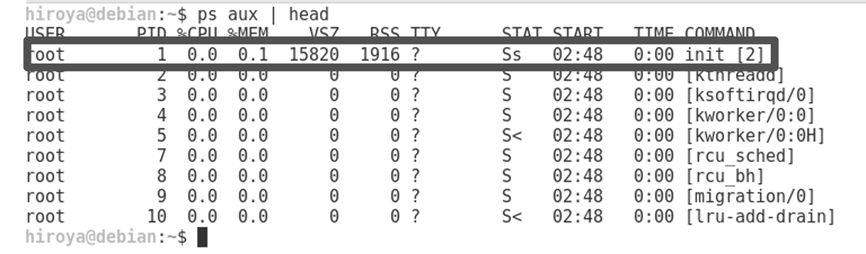
\includegraphics[keepaspectratio,width=0.5\hsize]{image201905-kansai/init01_gray.png}
 \\
  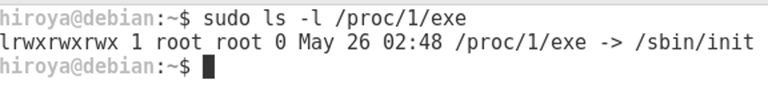
\includegraphics[keepaspectratio,width=0.5\hsize]{image201905-kansai/init02_gray.png}
 \\
  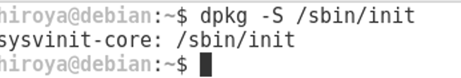
\includegraphics[keepaspectratio,width=0.3\hsize]{image201905-kansai/init03_gray.png}
 \\
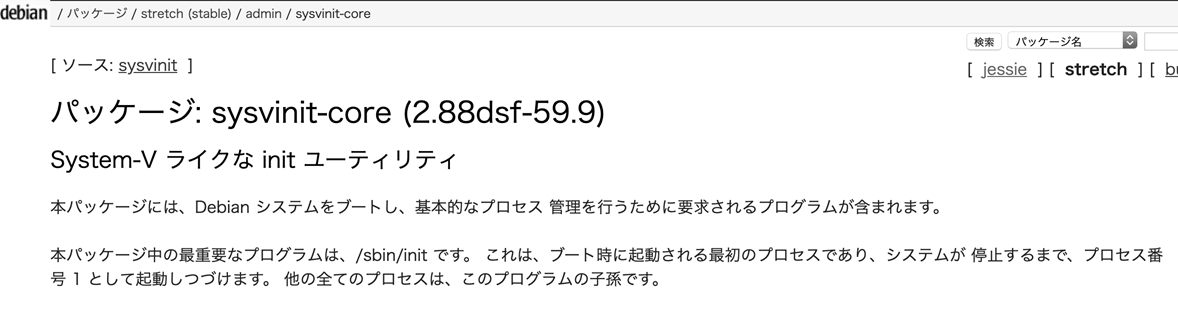
\includegraphics[keepaspectratio,width=0.7\hsize]{image201905-kansai/init04_gray.png}
\end{flushleft}

\subsection{Init$B%W%m%;%9$r8+$F$_$k(B(systemd)}
\begin{flushleft}
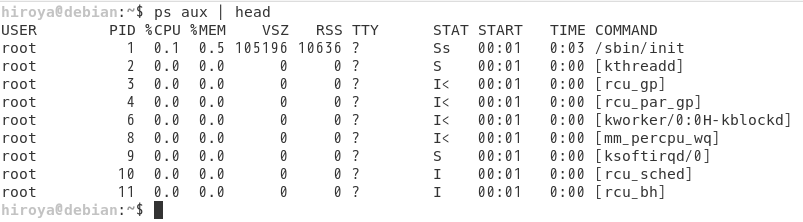
\includegraphics[keepaspectratio,width=0.5\hsize]{image201905-kansai/systemd01_gray.png}
 \\
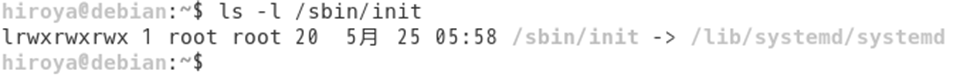
\includegraphics[keepaspectratio,width=0.5\hsize]{image201905-kansai/systemd02_gray.png}
 \\
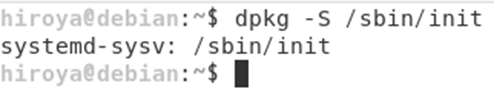
\includegraphics[keepaspectratio,width=0.3\hsize]{image201905-kansai/systemd03_gray.png}
 \\
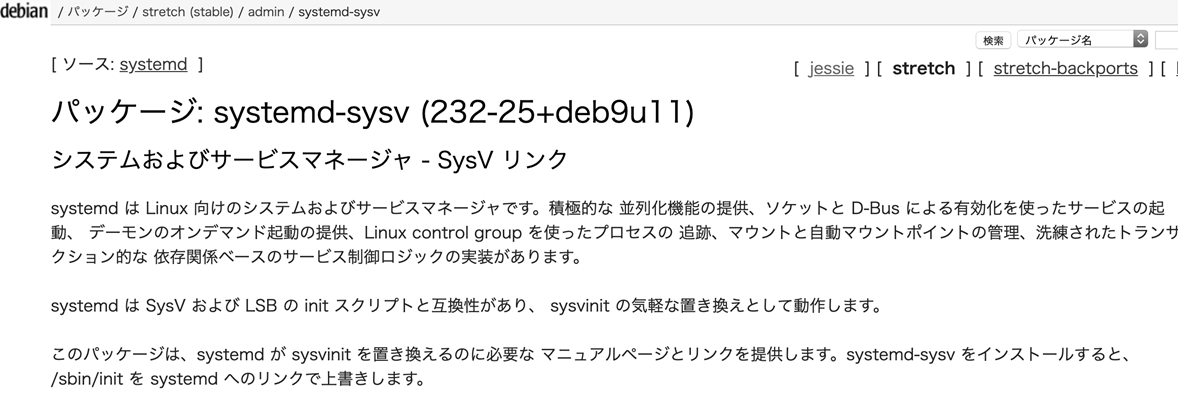
\includegraphics[keepaspectratio,width=0.7\hsize]{image201905-kansai/systemd04_gray.png}
\end{flushleft}

\subsection{systemd$B$N%a%j%C%H(B}
\subsubsection{$B$3$l$^$G$N(Binit$B%W%m%;%9$G$O0J2<$NLdBj$,H/@8$7$F$$$?(B}

\begin{itemize}
 \item $B%7%'%k%9%/%j%W%H$r=gHV$K<B9T$7$F$$$/$N$G!"%7%9%F%`$N5/F0$K;~4V$,$+$+$k(B
 \item $B%5!<%S%9$4$H$K(Bcgroups$B$G%j%=!<%9G[J,$rD4@0$9$k$J$I$N;EAH$_$,$J$$(B
\end{itemize}

\subsubsection{systemd$B$G$O!)(B}

\begin{itemize}
 \item $B%W%m%;%9$N5/F0$r=PMh$k8B$jJBNs$G9T$*$&$H$9$k$N$G!"5/F0$,Aa$$(B
 \item Cgroup$B$G%W%m%;%9$N4IM}$r9T$&$N$G!"%j%=!<%94IM}!"@8B83NG'$J$I$,=PMh$k(B
 \item $B%j%U%!%l%s%9$,$a$C$A$cCzG+$K=q$+$l$F$$$k(B
\end{itemize}

\subsection{sysvinit$B$N5/F0%W%m%;%9(B}
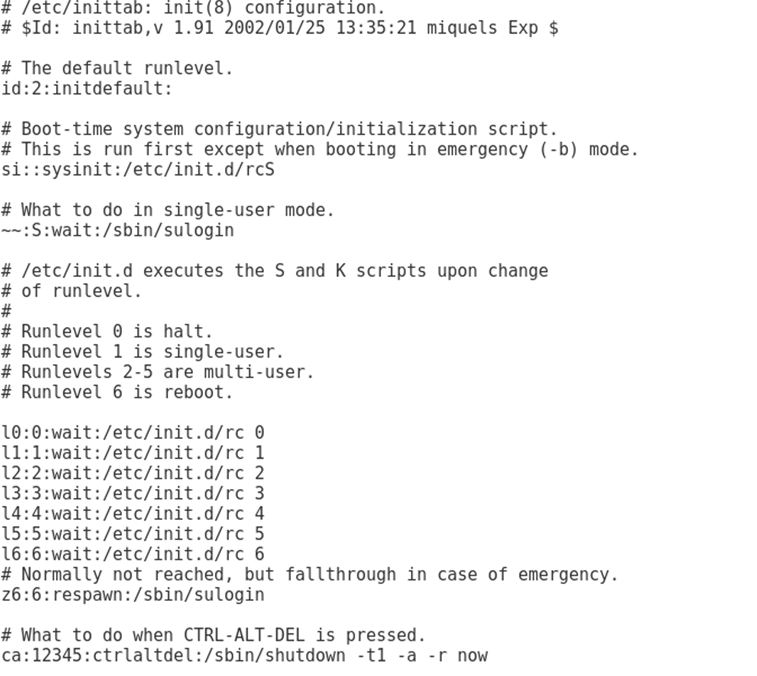
\includegraphics[keepaspectratio,width=0.5\hsize]{image201905-kansai/initboot01_gray.png}
 \\
/etc/init.d/rc
 \\
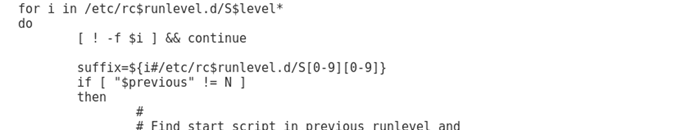
\includegraphics[keepaspectratio,width=0.5\hsize]{image201905-kansai/initboot02_gray.png}
 \\
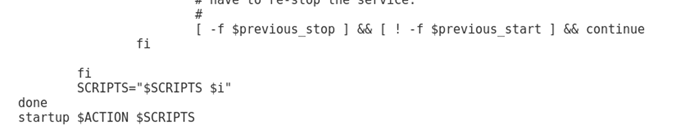
\includegraphics[keepaspectratio,width=0.5\hsize]{image201905-kansai/initboot03_gray.png}
 \\
/etc/rc*.d$B0J2<$N%9%/%j%W%H$r(B
$B=gHV$K<B9T$9$k(B
 \\
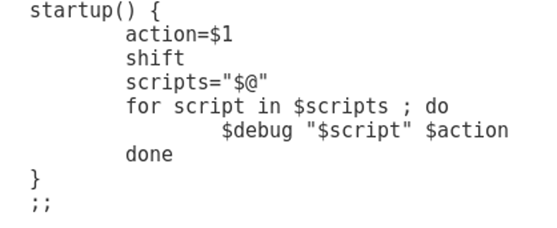
\includegraphics[keepaspectratio,width=0.5\hsize]{image201905-kansai/initboot04_gray.png}

\subsection{systemd$B$N5/F0%W%m%;%9(B}
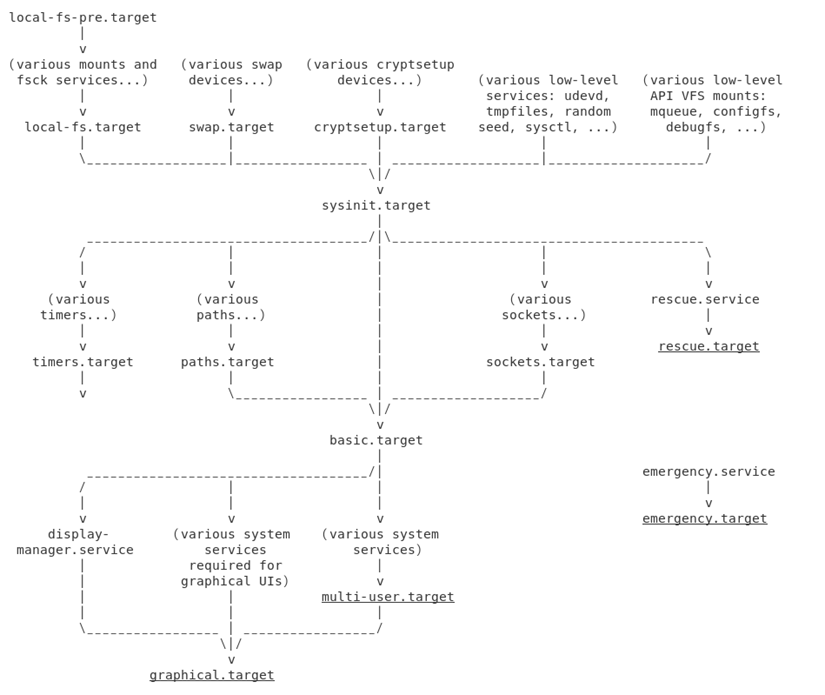
\includegraphics[keepaspectratio,width=0.5\hsize]{image201905-kansai/systemdboot01_gray.png}

\subsection{systemd$B$N%f%K%C%H(B}
systemd$B$O%W%m%;%9$r%f%K%C%H$H$$$&C10L$G4IM}$9$k(B
\\
$BA4It$G(B11$B8D$N%f%K%C%H$,B8:_$9$k(B
\begin{itemize}
 \item $B%5!<%S%9%f%K%C%H(B
 \item $B%?!<%2%C%H%f%K%C%H(B
 \item $B%=%1%C%H%f%K%C%H(B
 \item $B!D(B
\end{itemize}

\subsection{$B%5!<%S%9%f%K%C%H(B}
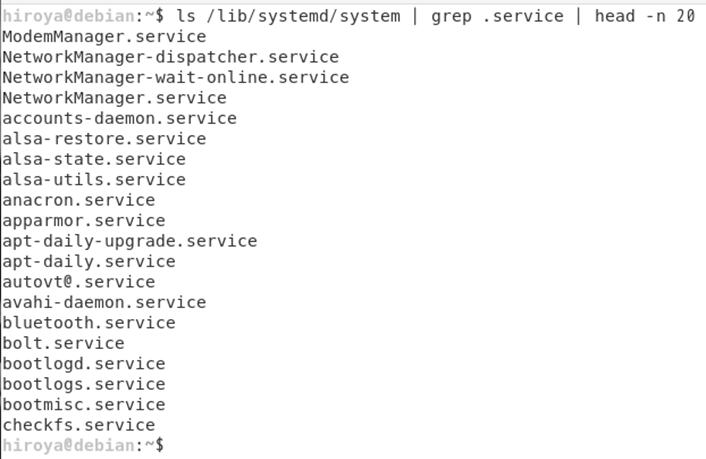
\includegraphics[keepaspectratio,width=0.5\hsize]{image201905-kansai/serviceunit01_gray.png}
\begin{itemize}
 \item $B%W%m%;%9$r@)8f!&4IM}$9$k$?$a$N%f%K%C%H(B
 \item .service$B$G=*$o$k%f%K%C%H%U%!%$%k(B
 \item $B0lHLE*$J%f!<%9%1!<%9$G;HMQ$9$k%f%K%C%H$O$[$H$s$I$3$l(B
\end{itemize}

\subsection{$B%?!<%2%C%H%f%K%C%H(B}
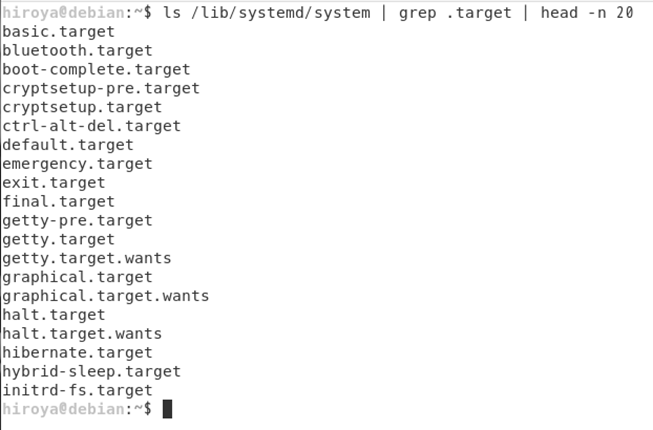
\includegraphics[keepaspectratio,width=0.5\hsize]{image201905-kansai/targetunit01_gray.png}
\begin{itemize}
 \item $BJ#?t$N%f%K%C%H$r%0%k!<%T%s%0$9$k$?$a$N%f%K%C%H(B
 \item .target$B$G=*$o$k%f%K%C%H%U%!%$%k(B
 \item $B%f%K%C%H4V$N5/F0=g=x$r$o$+$j$d$9$/$9$k$?$a$KMxMQ$5$l$k(B
\end{itemize}

\subsection{systemd$B$N5/F0=g=x(B}
$B%f%K%C%H$N4X78@-$O!V0MB8!W$H!V=g=x!W$N#2$D$N9M$(J}$,B8:_(B\\
$B0MB8(B
\begin{itemize}
 \item $B%W%m%;%9F1;N$,F1;~5/F0$9$k$+$I$&$+(B
 \item $B$"$/$^$G!"F1;~$K5/F0$9$k$+$I$&$+$G$"$j!"5/F0=g=x$O9MN8$7$J$$(B
\end{itemize}

$B=g=x(B
\begin{itemize}
 \item $B%W%m%;%95/F0$N=g=x4X78$rDj5A$9$k(B
\end{itemize}

$BNc$($P!"%W%m%;%9(BA$B$,%W%m%;%9(BB$B$rI,MW$H$9$k>l9g(B($B0MB8(B)$B!"(B
$BL@<(E*$K=g=x$r;XDj$7$J$$$H!"%W%m%;%9(BA$B$H(BB$B$OF1;~$K5/F0$9$k(B\\

$B$^$:!"(Bdefault.target$B$+$i0MB84X78!"=g=x4X78$r9=C[(B
 \\
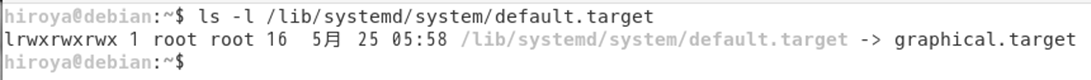
\includegraphics[keepaspectratio,width=0.5\hsize]{image201905-kansai/order01_gray.png}
 \\
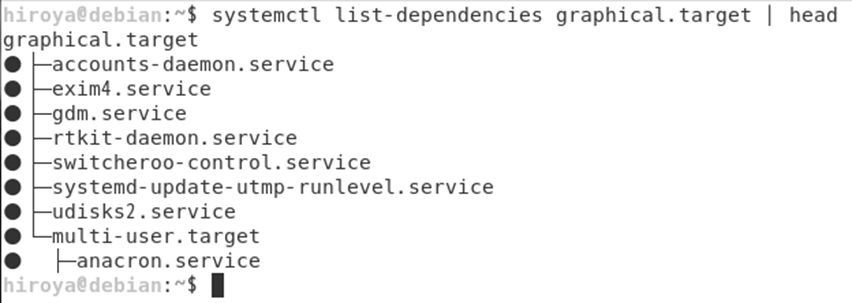
\includegraphics[keepaspectratio,width=0.5\hsize]{image201905-kansai/order02_gray.png}

\subsection{systemd$B$G$O$I$s$J%W%m%;%9$,5/F0$9$k$N!)(B}

sysvinit$B$G$O!"(B/etc/rc*.d$BFb$N%W%m%;%9$,5/F0$9$k(B\\
systemd$B$G$O!"0J2<$N%G%#%l%/%H%j$N%W%m%;%9$,5/F0BP>](B
\begin{itemize}
 \item /etc/systemd/system($B%f!<%6!<$N%3%s%U%#%0(B)
 \item /lib/systemd/system($B%$%s%9%H!<%k%Q%C%1!<%8$N%3%s%U%#%0(B)
\end{itemize}
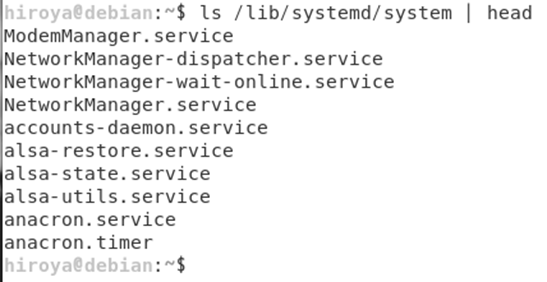
\includegraphics[keepaspectratio,width=0.5\hsize]{image201905-kansai/systemdsystem01_gray.png}

\subsection{systemctl$B$C$F!)(B}

systemd$B$K$"$l$3$l$HL?Na$r=P$9$3$H$,=PMh$k%3%^%s%I(B
\begin{itemize}
 \item systemctl status $B!D(B unit$B$N>uBV$r8+$k$3$H$,=PMh$k(B
 \item systemctl edit $B!D(B drop in$B$H$$$&5/F0$G(Bunit$B%U%!%$%k$rJT=8(B
 \item systemctl show/cat $B!D(B unit$B%U%!%$%k$rI=<((B
 \item systemctl enable/disable $B!D(B $B%W%m%;%9$N<+F05/F0$r@)8f(B
 \item systemctl daemon-reload $B!D(B unit$B%U%!%$%k$NJQ99$rH?1G(B
 \item systemctl start/stop/restart $B!D(B $B%W%m%;%9$N5/F0@)8f(B
 \item systemctl list-unit-files --type=service $B!D(B $B%5!<%S%9$N0lMw$rI=<((B
\end{itemize}

\subsection{$B<B:]$K%5!<%S%9$r:n$C$F$_$k(B($B<+F05/F0(B)}
sampleA.service
\begin{commandline}
[Service]
ExecStart=/bin/bash -c "date > /home/hiroya/sampleA.txt; sleep 10"

[Install]
RequiredBy=multi-user.target
\end{commandline}
$B8=:_$NF|;~$r(BsampleA.txt$B$N=PNO$9$k%W%m%;%9(B\\
multi-user.taget$B$N5U0MB8$r;XDj(B
 \\
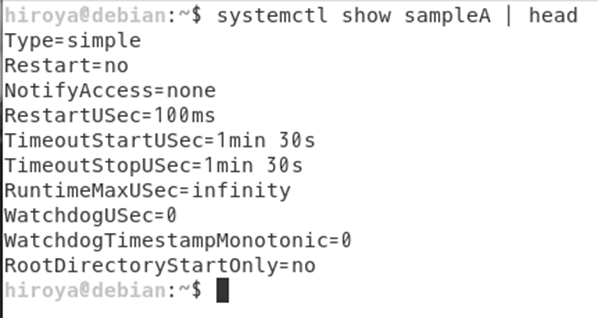
\includegraphics[keepaspectratio,width=0.5\hsize]{image201905-kansai/samplea01_gray.png}
 \\
sampleA$B$NL@<(E*$J@_Dj$O(B2$B9T$@$1$@$,!"8e$m$G$$$m$$$m$J@_Dj$,>!<j$KIUM?$5$l$k(B

\subsection{$B<+F05/F0$NM-8z2=(B}
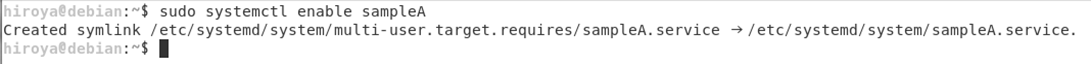
\includegraphics[keepaspectratio,width=0.5\hsize]{image201905-kansai/samplea02_gray.png}
 \\
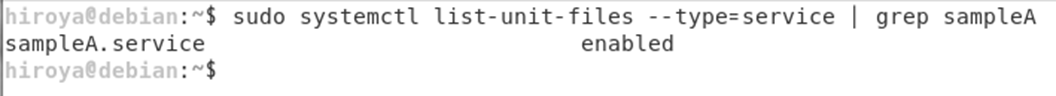
\includegraphics[keepaspectratio,width=0.5\hsize]{image201905-kansai/samplea03_gray.png}

\subsection{$B<B:]$K%5!<%S%9$r:n$C$F$_$k(B($B0MB8$"$j(B)}
sampleA.service

\begin{itemize}
 \item sampleB.service$B$X$N0MB8$rDI2C(B
 \item sampleA$B$K$O!"(BsampleB$B$,I,MW$H$$$&$3$H(B
\end{itemize}

\begin{commandline}
[Unit]
Requires=sampleB.service

[Service]
ExecStart=/bin/bash -c "date > /home/hiroya/sampleA.txt; sleep 10"

[Install]
RequiredBy=multi-user.target

\end{commandline}
sampleB.service
\begin{commandline}
[Service]
ExecStart=/bin/bash -c "date > /home/hiroya/sampleB.txt"
\end{commandline}
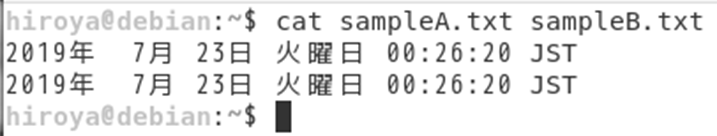
\includegraphics[keepaspectratio,width=0.5\hsize]{image201905-kansai/samplea04_gray.png}
 \\
sampleA$B$+$i(BsampleB$B$,8F$S=P$5$l$F$$$k$3$H$,$o$+$k(B
$B$^$?!"0MB8$N$_$J$N$G!"(BsampleA$B$H(BsampleB$B$OF1;~$K5/F0$7$F$$$k(B

\subsection{$B<B:]$K%5!<%S%9$r:n$C$F$_$k(B($B=g=x$"$j(B)}
sampleA.service
\begin{commandline}
[Unit]
Requires=sampleB.service
Before=sampleB.service

[Service]
Type=oneshot
ExecStart=/bin/bash -c "date > /home/hiroya/sampleA.txt; sleep 10"

[Install]
RequiredBy=multi-user.target
\end{commandline}
Before$B$H(BType=oneshot$B$rDI2C$9$k$3$H$G!"(B
sampleA$B$N8e$K!"(BsampleB$B$r5/F0$9$k$3$H$,=PMh$k(B
 \\
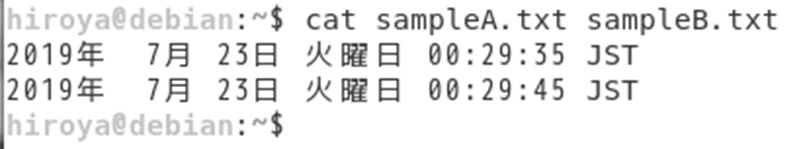
\includegraphics[keepaspectratio,width=0.5\hsize]{image201905-kansai/samplea05_gray.png}
 \\
sampleA$B$N(B10$BIC8e$K(BsampleB$B$,5/F0$7$F$$$k$3$H$,$o$+$k(B

\subsection{$B$*$^$1(B}

\subsection{journalctl$B$C$F!)(B}
\begin{itemize}
 \item systemd$B4D6-$G$O!"%m%0$N<}=8$O(Bjournald(system-journald)$B$,C4Ev(B
 \item journalctl$B$O(Bjournald$B$KBP$7$FL?Na$r9T$&;v$,$G$-$k%3%^%s%I(B
 \item Systemd$B$N%5!<%S%9$N%m%0$rI=<($G$-$k$N$G!"%(%i!<$N:]$OJXMx(B
\end{itemize}
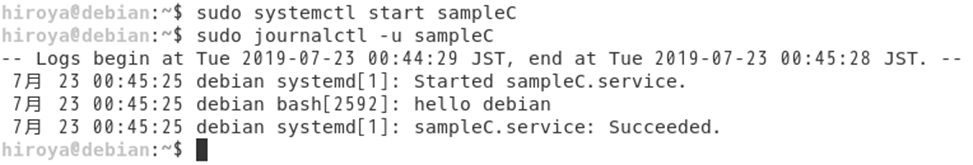
\includegraphics[keepaspectratio,width=0.5\hsize]{image201905-kansai/journalctl01_gray.png}

\subsection{graphical.target$B$NA+0\$r<YKb$7$F$_$k(B}
sample.service
\begin{commandline}
[Unit]
Before=sysinit.target
DefaultDependencies=no
OnFailure=emergency.target

[Service]
Type=oneshot
ExecStart=/bin/false

[Install]
RequiredBy=sysinit.target
\end{commandline}
sysinit.target$B$,40N;$;$:!"<!$N%?!<%2%C%H$KA+0\$;$:$K!"(B
$B6/@)E*$K(Bemergency.target$B$KA+0\$9$k(B\\
systemd$B$N5/F0%W%m%;%9(B($B:F7G(B)
 \\
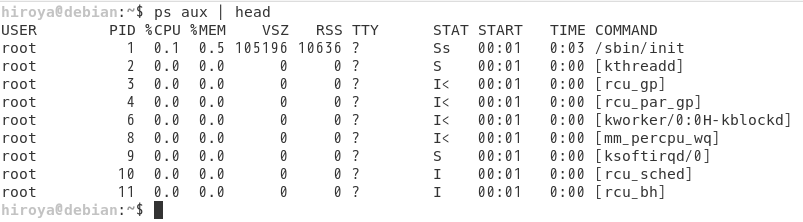
\includegraphics[keepaspectratio,width=0.5\hsize]{image201905-kansai/systemd01_gray.png}


sample.service
\begin{commandline}
[Unit]
Before=sysinit.target
DefaultDependencies=no
#OnFailure=emergency.target

[Service]
Type=oneshot
ExecStart=/bin/false

[Install]
RequiredBy=sysinit.target
\end{commandline}
OnFailure$B$r%3%a%s%H%"%&%H$9$k$H!"@5>o$K(BOS$B$,5/F0$7$J$/$J$k(B
($B%W%m%s%W%H<uIU$r$7$J$/$J$k(B)\\
$B$b$7!"(Bsysinit.target$B$h$j$bA0$N%5!<%S%9$r:n@.$9$k>l9g$O!"(B
OnFailure$B$r@_Dj$7$F$*$/$H0B?4(B

%$B$4@6D0$"$j$,$H$&$4$6$$$^$7$?(B


%201907 tokyo
\dancersection{Buster $B%G%9%/%H%C%W$NF|K\8lF~NO(B}{yy\_y\_ja\_jp}

Debian $B$NF|K\8lF~NO$O(Buim-mozc$B$,%G%U%)%k%H(B\footnote{$B0lIt$N%"!<%-%F%/%A%c$O(Buim-anthy}$B$G!"$*9%$_$G(Bibus$B$d(Bfcitx$B$J$I!"(Banthy$B$d(Bskk$B$J$I$b;H$($^$9!#(BStretch (9) $B$^$G$HF1MM$K(B Buster (10) $B$G$b$U$D$&$K;H$($k$h$&$K!"(Bim-config$B$H$$$&%Q%C%1!<%8$GBP1~$r9T$$$^$7$?!#(B

Debian $B$OD9$i$/(BGNOME$B$,%G%U%)%k%H%G%9%/%H%C%W$G$9!#(BStretch$B$G$O?^(B\ref{fig:desktop-stretch}$B$N$h$&$J46$8$G$7$?!#(BBuster$B$G$O?^(B\ref{fig:desktop-buster}$B$N$h$&$K$J$j!"$"$^$jJQ$o$C$F$$$J$$$h$&$K8+$($^$9!#$7$+$7!"Cf?H$O$+$J$jJQ$o$j$^$7$?!#(B

\begin{figure}[h]
\begin{center}
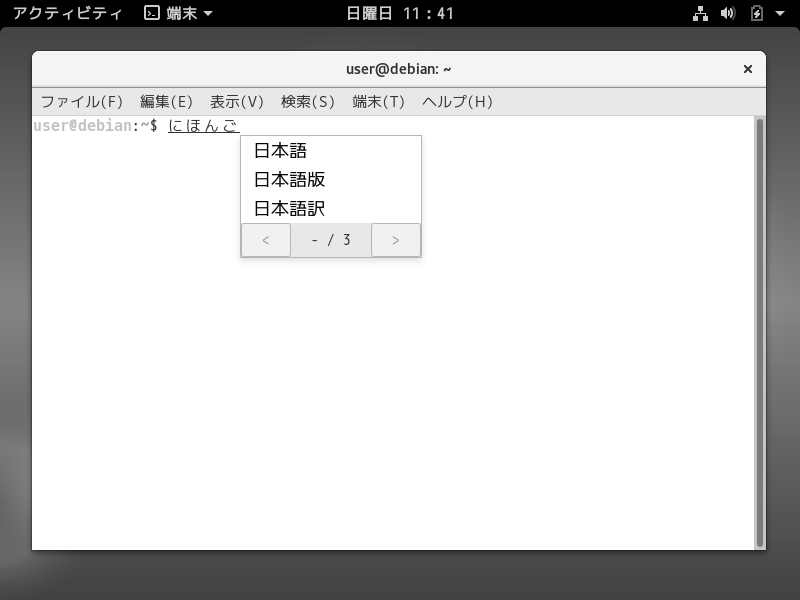
\includegraphics[keepaspectratio,width=0.45\hsize]{image201907/stretch_gnome_3_gray.png}
\end{center}
\caption{Stretch $B$N%G%U%)%k%H%G%9%/%H%C%W(B}
\label{fig:desktop-stretch}
\end{figure}

\begin{figure}[h]
\begin{center}
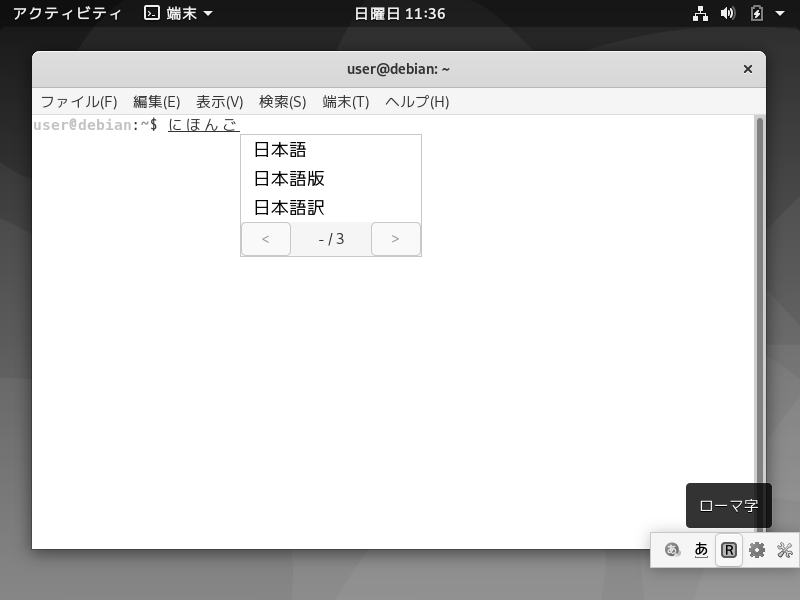
\includegraphics[keepaspectratio,width=0.45\hsize]{image201907/buster_gnome_3_gray.png}
\end{center}
\caption{Buster $B$N%G%U%)%k%H%G%9%/%H%C%W(B}
\label{fig:desktop-buster}
\end{figure}

$BFC$KJQ$o$C$?$N$O(BGNOME$B$G!"(BStretch$B$^$G$O(BGNOME on Xorg$B$,%G%U%)%k%H$G$7$?$,!"(BBuster$B$G$O(BGNOME on Wayland$B$,%G%U%)%k%H$K$J$j$^$7$?!#(B
Wayland$B$G$O(BXorg$B$G9T$o$l$F$$$?@_Dj$,2?$b$5$l$J$$$J$IMM!9$JLdBj$,$"$j$^$7$?$,!"4pK\E*$K$O;H$($k$h$&$K$7$^$7$?!#(B

\subsection{$B%G%U%)%k%H%G%9%/%H%C%W(B}
Debian$B%$%s%9%H!<%i$N%=%U%H%&%'%"A*Br2hLL$G$OJ#?t$N%G%9%/%H%C%W4D6-$rA*$Y$^$9$,!J?^(B\ref{fig:d-i-tasksel}$B!K!"$=$N$&$A0lHV>e$K$"$k$b$N$,%G%U%)%k%H%G%9%/%H%C%W$H8F$P$l$F$$$^$9!#(B
$B$J$*$3$N2hLL$GA*$Y$k%G%9%/%H%C%W4D6-$O!"(BBuster $B$G$O(B LXQt $B$,2C$o$C$?0J30$OFC$KJB$S=g$bJQ$o$C$F$$$^$;$s!#(B

\begin{figure}[h]
\begin{center}
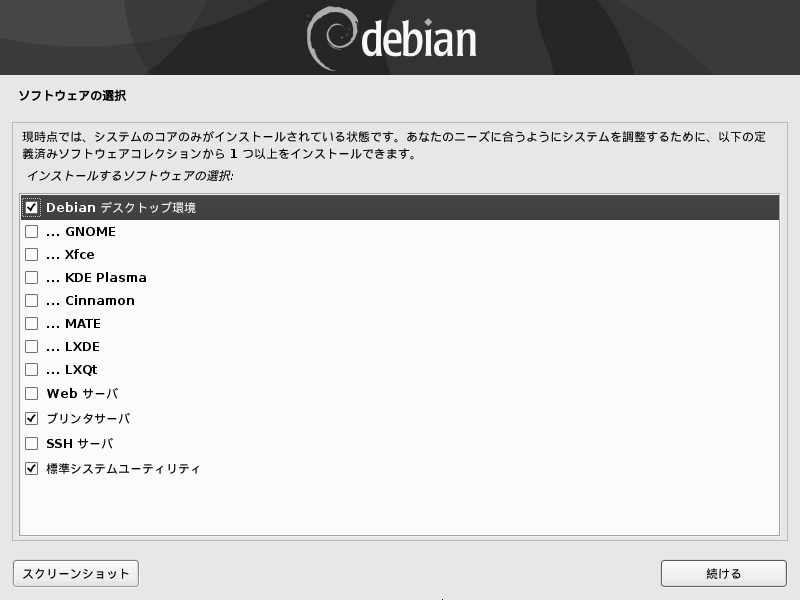
\includegraphics[keepaspectratio,width=0.7\hsize]{image201907/buster_tasksel_0_gray.png}
\end{center}
\caption{Debian $B%$%s%9%H!<%i$N%=%U%H%&%'%"A*Br2hLL(B}
\label{fig:d-i-tasksel}
\end{figure}

$B$3$3$G(BGNOME$B$K$b%A%'%C%/$rF~$l$F?J$`$H!"(BGNOME$B%G%9%/%H%C%W$H$H$b$K%m%0%$%s2hLL$N%G%#%9%W%l%$%^%M!<%8%c(Bgdm3$B$,%$%s%9%H!<%k$5$l$^$9!#(B

$B%$%s%9%H!<%k40N;8e$K5/F0$9$k$H(Bgdm3$B$N%m%0%$%s2hLL$K$J$j$^$9!#%f!<%6!<$rA*Br$9$k$H%Q%9%o!<%IF~NO2hLL$K$J$j$^$9$,!"$3$3$G(BStretch$B$N(BGNOME$B$+$iJQ$o$C$?$H$3$m$,$"$j$^$9!#%5%$%s%$%s%\%?%s$N:8NY$K$"$k;u<V$r%/%j%C%/$9$k$H!"(BStretch $B$N%m%0%$%s2hLL$G$O?^(B\ref{fig:gdm3-stretch}$B$N$h$&$K(B ``System X11 Default''$B$,A*Br$5$l$F$*$j!"$^$?0lHV2<$N%a%K%e!<$O(B ``GNOME on Wayland''$B$H$J$C$F$$$^$7$?!#$7$+$7(BBuster$B$G$O?^(B\ref{fig:gdm3-buster}$B$N$h$&$K0l8+(BStretch$B$N$H$-$K$b$"$C$?$h$&$J%a%K%e!<$N(B ``GNOME'' $B$,A*Br$5$l$F$*$j!"$^$?0lHV2<$N%a%K%e!<$,(B ``GNOME on Xorg''$B$K$J$C$F$$$^$9!#F1$8%a%K%e!<L>(B ``GNOME''$B$G$b(BStretch$B$^$G$O<BBN$,(BGNOME on Xorg$B$G$7$?$,!"(BBuster$B$N$b$N$O(BGNOME on Wayland$B$K$J$C$?$N$G$9!#(B

\begin{figure}[h]
\begin{center}
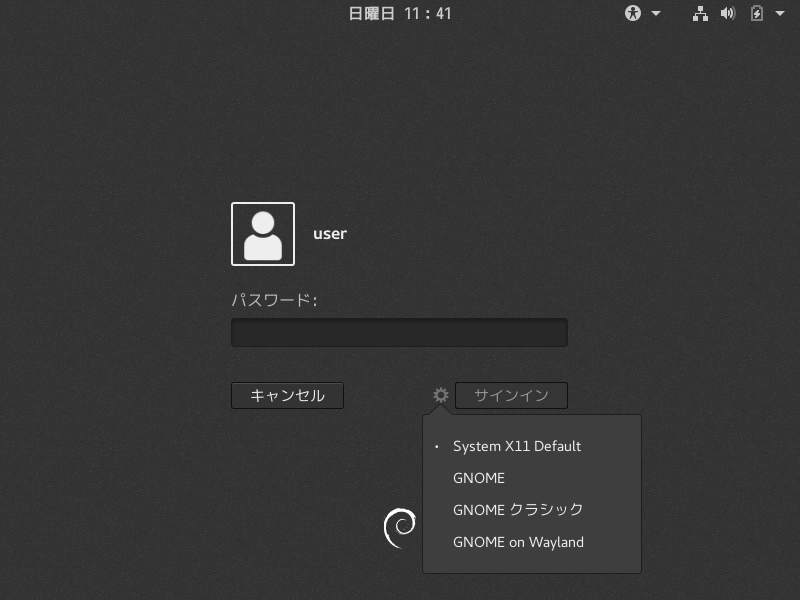
\includegraphics[keepaspectratio,width=0.7\hsize]{image201907/stretch_gnome_0_gray.png}
\end{center}
\caption{Stretch $B$N%m%0%$%s2hLL(B}
\label{fig:gdm3-stretch}
\end{figure}

\begin{figure}[h]
\begin{center}
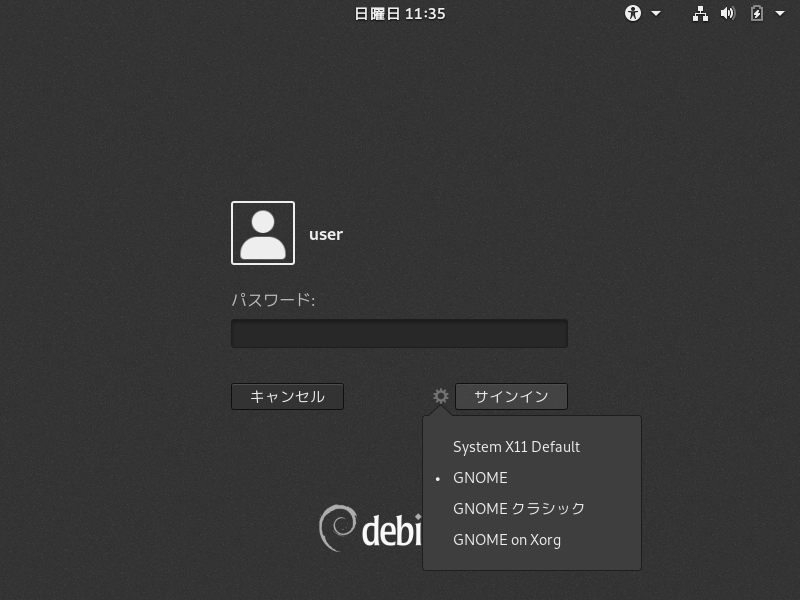
\includegraphics[keepaspectratio,width=0.7\hsize]{image201907/buster_gnome_0_gray.png}
\end{center}
\caption{Buster $B$N%m%0%$%s2hLL(B}
\label{fig:gdm3-buster}
\end{figure}

$B$D$^$j%G%U%)%k%H%G%9%/%H%C%W$,(BGNOME$B$G$"$k$3$H$OJQ$o$C$F$$$^$;$s$,!"@53N$K$O(B

\begin{itemize}
 \item Stretch $B$^$G$O(B GNOME on Xorg
 \item Buster $B$G$O(B GNOME on Wayland
\end{itemize}

$B$H$J$C$F$$$^$9!#(B

\subsection{Stretch $B$^$G$N(B im-config}
$BF|K\8l$J$I$rF~NO$9$k$K$OF~NO%a%=%C%I%U%l!<%`%o!<%/$HF~NO%a%=%C%I%(%s%8%s$N@_Dj$,I,MW$G$9!#$3$N@_Dj$O(BGTK+$B$d(BQt$B$H$$$C$?(BGUI$B%i%$%V%i%j!"$b$7$/$O(BXIM (X Input Method)$B$KBP$7$F9T$&I,MW$,$"$j!"Nc$($P(BGTK+$B$G$O(B\verb|GTK_IM_MODULE| $B$H$$$C$?4D6-JQ?t$,;H$o$l$F$$$^$9!#$^$?!"F~NO$rJQ49$9$k$?$a$NJd=u%D!<%k$N%G!<%b%s$d!"F~NO%a%=%C%I$N>uBV$rI=<($9$k$?$a$N%D!<%k%P!<$J$I$r5/F0$9$kI,MW$,$"$j$^$9!#(B
Debian$B$K$OF~NO%a%=%C%I%U%l!<%`%o!<%/$,(Buim$B!"(Bibus$B!"(Bfcitx$B$J$IJ#?t$"$j!"F|K\8l4D6-$N%G%U%)%k%H$O(Buim$B$G$9$,$*9%$_$GA*$V$3$H$,$G$-$^$9!#$^$?(BDebian$B$K$O%G%9%/%H%C%W$b(BGNOME$B$K8B$i$:$?$/$5$s$"$j<+M3$KA*$Y$^$9!#$I$N%G%9%/%H%C%W$rA*$s$G$b!"$=$7$F$I$NF~NO%a%=%C%I%U%l!<%`%o!<%/$rA*$s$G$b!"%$%s%9%H!<%k$7$?$i2?$b?($i$J$/$F$b%G%U%)%k%H$G$3$N$h$&$J@_Dj$d5/F0$,$5$l$k$h$&$K!"%7%'%k%9%/%j%W%H$G=q$+$l$?(Bim-config$B%Q%C%1!<%8$,<+F0@_Dj$7$F$/$l$^$9!#<+F0@_Dj$5$l$kCM$O%$%s%9%H!<%k$5$l$F$$$k%Q%C%1!<%8$d%m%0%$%s%f!<%6!<$N;H$&8@8l$r$b$H$KF0E*$KJQ$o$j$^$9!#$J$*!"$*9%$_$G(Bim-config$B$r<jF0$G%f!<%6!<Kh$d%7%9%F%`A4BN$K@_DjJQ99$7$?$j!"(Bim-config$B$r;H$o$:$9$Y$F<jF0$G@_Dj$9$k$3$H$b$G$-$k$h$&$K$J$C$F$$$^$9!#(B

Stretch$B$^$G$N(Bim-config$B$K$D$$$F>\$7$/$O(B2013$BG/2F9f$N5-;v(B\footnote{\url{https://tokyodebian-team.pages.debian.net/pdf2013/debianmeetingresume2013-natsu.pdf}}$B$r$4Mw$/$@$5$$!#Ev;~$O(BWheezy (7.0)$B$G$7$?$,Bg$-$/$OJQ$o$C$F$$$^$;$s!#(B

%XXX config dependencies

\subsection{XIM $B$H(B GUI$B%i%$%V%i%j(B}
im-config$B$O(BXIM$B4XO"$GBg$-$/(B2$B$D$N@_Dj$r$7$F$-$^$7$?!#(B

1$B$DL\$O(BXIM$B$X$N@_Dj!"(B\verb|XMODIFIERS| $B4D6-JQ?t$G$9!#$3$l$O<g$K(BXIM$B$GF~NO$rD>@\07$&!J(BGUI$B%i%$%V%i%j$r;H$o$J$$!K%"%W%j%1!<%7%g%s!"Nc$($P(Bxterm$B$J$I8~$1$N@_Dj$G$9$,!"(B2$B$DL\$N@_Dj$H$b4XO"$,$"$j$^$9!#(B

2$B$DL\$O(BGUI$B%i%$%V%i%j$KBP$9$k@_Dj$G$9!#(Buim$B$J$I$NF~NO%a%=%C%I%U%l!<%`%o!<%/$O(BGUI$B%i%$%V%i%j$=$l$>$l$K%W%i%0%$%s$rDs6!$9$kI,MW$,$"$j!"$=$l$,%$%s%9%H!<%k$5$l$F$$$l$P(BGUI$B%i%$%V%i%j$OD>@\(Buim$B$J$I$HDL?.$G$-$^$9!#$?$@!"$=$l$,%$%s%9%H!<%k$5$l$F$$$J$/$F$b(BGUI$B%i%$%V%i%j$O(BXIM$B$HDL?.$9$k5!G=$,$"$j$^$9!#(BGTK+$B$N>l9g$O(B\verb|GTK_IM_MODULE=xim|$B$H$9$l$P(BXIM$B$HDL?.$7$^$9!#(B1$B$DL\$N@_Dj$HAH$_9g$o$;$k$3$H$G!"(BGTK+$B$O(BXIM$B7PM3$G(Buim$B$J$I$HDL?.$9$k$3$H$,2DG=$G$9!#(B

$B$7$+$7!"(BXIM$B$K$h$kF~NO$OFCDj$N>r7o$G%U%j!<%:$7$?$j$H$&$^$/F0$+$J$$$3$H$,$"$k$3$H$,CN$i$l$F$$$^$7$?!#(B

\subsection{Stretch $B$^$G$N(B uim}
2017$BG/E_9f$N5-;v(B ``Debian Stretch$B$N%$%s%W%C%H%a%=%C%I$N8=>u(B'' \footnote{\url{https://tokyodebian-team.pages.debian.net/pdf2017/debianmeetingresume2017-fuyu.pdf}}$B$G$b<h$j>e$2$i$l$F$$$^$7$?$,!"?^(B\ref{fig:desktop-stretch}$B$b8+$k$H$o$+$j$^$9$,(BStretch$B$N(BGNOME$B$G$O(Buim$B$N>uBV$,2hLL>e$G8+$($^$;$s!#(BKDE$B$J$I$[$+$N%G%9%/%H%C%W$G$b8+$($J$$!"$J$$$7$o$+$j$K$/$$$b$N$,$"$j$^$7$?!#(BGNOME$B$d(BKDE$B$J$I%G%9%/%H%C%W$J$I$,JQ2=$7$F$$$C$?$3$H$,860x$+$H$_$i$l$^$9!#(B

\subsection{GNOME}
Debian$B$O(BWheezy$B$G(BGNOME 3$B$r<h$j9~$_$^$7$?$,!"$=$l$h$jA0$K$"$C$?(BGNOME 2$B$H$OBg$-$/0[$J$j$^$9!#(BGNOME $B%7%'%k$H$$$&$b$N$rF3F~$7!"%G%9%/%H%C%W$G$OI8=`E*$J%7%9%F%`%H%l%$$rGQ;_$7$F%H%C%W%P!<!J2hLL:G>eIt$N9u$$%P!<!K$KCV$-49$($^$7$?!#$=$N$?$a:#$^$G%7%9%F%`%H%l%$$KI=<($7$F$$$?(Buim$B$N>uBV$O8+$($J$/$J$C$F$7$^$$$^$7$?!#$=$7$F%H%C%W%P!<$KI=<($9$k$K$O(BGNOME 3$BFH<+$N(BJavaScript API$B$GIA2h$7$J$1$l$P$J$i$:BP1~$r$`$:$+$7$/$7$F$$$^$9!#(B

$B$5$i$K!"(BWheezy$B$K$O(BGNOME 3.4$B!"(BJessie (8) $B$K$O(BGNOME 3.14$B$r4^$s$G$$$^$7$?$,!"%P!<%8%g%s(B3.5$B:"$+$i(BGNOME$B$OF~NO%a%=%C%I%U%l!<%`%o!<%/$H$7$F(Bibus$B$rAH$_9~$_$O$8$a$?$h$&$G!"(BGNOME$B$OFH<+(BD-Bus API$B$r(Bibus$B@lMQ$KDs6!$7$FDL?.$7$F$$$k$h$&$G!"(B\verb|GTK_IM_MODULE|$B4D6-JQ?t$,@_Dj$5$l$F$$$J$/$F$b(BGTK+$B$G(Bibus$B$,F0:n$9$k$h$&$G$9!#(Bibus$B0J30$r;H$&$3$H$b$G$-$k$H5-$5$l$F$O$$$k$b$N$N!"(Bibus-daemon$B$,:o=|$5$l$F$$$l$P;H$($k$H$5$l$F$$$^$9(B\urldef{\gnomeibusurl}\url{https://wiki.gnome.org/ThreePointFive/Features/IBus#How_to_use_other_IM_frameworks}\footnote{\gnomeibusurl}$B!#$D$^$j(BGNOME$B$G(Buim$B$d(Bfcitx$B$J$I(Bibus$B0J30$r;H$&$K$O!"(Bim-config$B$J$I$N@_Dj$r@Z$jBX$($k$@$1$G$J$/!"(Bibus-daemon$B$H$$$&%P%$%J%j!J$D$^$j(B \verb|/usr/bin/ibus-daemon|$B!K$r4^$s$G$$$k(Bibus$B%Q%C%1!<%8$r:o=|$7$J$$$HF0:nJ]>Z$5$l$J$$!"$H$$$&%b%8%e!<%k2=$H$O??5U$NJ}8~@-$G;DG0$J>u67$G$9!#<B:]!"(Buim$B$d(Bfcitx$B$NF0:nCf$K(Bibus$B%Q%C%1!<%8$,%$%s%9%H!<%k$5$l$?$^$^$@$H(Bibus$B$r;H$C$F$$$J$$$N$K%H%C%W%P!<$NI=<($,$*$+$7$/$J$C$?$j!"%-!<F~NO$K(Bibus$B$,F1;~$KH?1~$7$?$j$H$$$&$3$H$b5/$3$C$?$j$9$k$h$&$G$9!#(B

$B$=$7$F@h$[$I8+$?$H$*$j!"(BStretch$B%j%j!<%9$h$j8e$K:#$^$G$N(BXorg$B$KBe$o$j(BWayland$B$r%G%U%)%k%H$K$7$?$h$&$G$9(B\footnote{$B@53N$K$O(BStretch$B$KF~$C$F$$$k(BGNOME 3.22$B$G(BGNOME$BK\2H$O(BWayland$B%G%U%)%k%H$K$7$?$b$N$N!"(BDebian$B$O(BXorg$B%G%U%)%k%H$KLa$7$F$$$?$h$&$G$9(B(gnome-session 3.21.90-3)$B!#(BStretch$B$,%j%j!<%9$5$l$?$N$GK\2H$K9g$o$;$F(BWayland$B%G%U%)%k%H$K$7$?$h$&$G$9!#(B}$B!#(BGNOME $B%7%'%k$OL@$i$+$K(BWayland$B$N>l9g$K5!G=@)8B$7$F$$$^$9!#(BGTK+$B$K$O%&%#%s%I%&$r(BAlt+Tab$B$d%?%9%/%P!<$H$$$C$?%&%#%s%I%&0lMw$KI=<($7$J$$$h$&$K$9$k@_Dj(B\urldef{\gtktaskbarurl}\url{https://developer.gnome.org/gtk3/stable/GtkWindow.html#gtk-window-set-skip-taskbar-hint}\footnote{$B@53N$K$O%G%9%/%H%C%W4D6-$KBP$7$F%?%9%/%P!<$KI=<($7$J$$$h$&MW@A$9$k5!G=$G$9!#(B\\
\gtktaskbarurl}$B$,$G$-$k$N$G$9$,!"(BWayland$B>e$G$O$3$N@_Dj$rL5;k$7$^$9(B\footnote{\url{https://bugzilla.gnome.org/show_bug.cgi?id=771329}}$B!#$=$N$?$a(BGNOME on Wayland$B$G$O%D!<%k%P!<%&%#%s%I%&$,(BAlt+Tab$BBP>]$K$J$C$F$7$^$$F~NO$7$E$i$/$J$j$^$9!#$*$=$i$/$=$s$J%D!<%k%P!<$J$IGQ;_$7$F$7$^$C$F%H%C%W%P!<1&B&$K$G$b(BGNOME 3$BFH<+$N(BJavaScript API$B$GIA2h$;$h$H$$$&<gD%$J$N$G$7$g$&!#$7$+$7$=$l$G$OB>$N%G%9%/%H%C%W$,:$$j$^$9!#(B

Wayland$B<+BN$K$D$$$F$O8e$K$^$H$a$^$9!#(B

\subsection{KDE}
Debian$B$O(BStretch$B$G(BKDE 5$B$r<h$j9~$_$^$7$?!#(Buim$B$K$O%7%9%F%`%H%l%$$N$[$+$K(BKDE 4$B8~$1$N(BPlasma$B%&%#%8%'%C%H$,$"$j$^$9$,!"(BKDE 5$B$G$O8_49@-$,$J$/F0:n$7$^$;$s!#(B

$B$J$*(BKDE 5$B$K$O(Bkimpanel$B$H$$$&F~NO%a%=%C%I$N>uBVI=<(MQ(BPlasma$B%&%#%8%'%C%H$,I8=`$GAH$_9~$^$l$F$*$j!"%?%9%/%P!<$NCf$K$b:G=i$+$iI=<($5$l$F$$$^$9!#(Bfcitx$B3+H/<T$,:n$C$?$h$&$G!"(Bfcitx-module-kimpanel$B%Q%C%1!<%8$r%$%s%9%H!<%k$9$l$P(Bfcitx$B$N>uBV$rI=<($G$-$k$h$&$G$9!#(Bfcitx$B0J30$NF~NO%a%=%C%I%U%l!<%`%o!<%/$G$b(Bkimpanel$B$N%W%m%H%3%k$GDL?.$7$5$($9$l$P(Bkimpanel$B$K>uBVI=<($G$-$k$h$&$G$9!#$5$i$K$3$N(Bkimpanel$B%W%m%H%3%k$r;H$C$F(BGNOME 3$B$G$b>uBVI=<($9$Y$/(BGNOME $B%7%'%k3HD%(Bgnome-shell-extension-kimpanel$B%Q%C%1!<%8$r:n$C$?$h$&$G$9!#$3$l$r;H$($P(BGNOME 3$BFH<+$NIA2h$rF~NO%a%=%C%I%U%l!<%`%o!<%/$=$l$>$l$,4hD%$i$:$K:Q$`$+$b$7$l$^$;$s!#(B

$B$^$?(BKDE$B$b(BWayland$BBP1~$r?J$a$F$$$k$h$&$G!"(Bplasma-workspace-wayland$B%Q%C%1!<%8$r%$%s%9%H!<%k$9$k$H;n$9$3$H$,$G$-$^$9(B\footnote{$B8e=R$7$^$9$,8=;~E@$G$O$3$N>e$G5/F0$5$l$k%"%W%j%1!<%7%g%s$O%G%U%)%k%H(BXWayland$B$GF0:n$7$F$$$k$h$&$G$9!#(B}$B!#(B

\subsection{Wayland -- Xorg $B$H$N0c$$(B}
Xorg$B$O@N$+$i$"$j$^$9$,!"(BWayland$B$O8eH/$H$7$F%G%#%9%W%l%$%5!<%P$r0l$+$i:n$jD>$7$?$h$&$G$5$^$6$^$J5!G=$r$*$=$i$/$"$($F:o$C$F$$$k$h$&$G$9!#(B

\begin{itemize}
 \item $B%;%C%7%g%s$N=i4|2=(B
 \begin{itemize}
  \item $B4D6-JQ?t$J$I$N@_Dj(B
  \item $B%G!<%b%s$J$I$N5/F0(B
 \end{itemize}
 \item $B%&%#%s%I%&$NG[CV(B
 \begin{itemize}
  \item $B0LCV>pJs$N<hF@!&@_Dj(B
  \item $B:GA0LLI=<($J$IA08e4X78$N@_Dj(B
 \end{itemize}
\end{itemize}

Xorg$B$NI|=,$b$7$J$,$i!"$=$l$>$l$NBP:v0F$b$^$H$a$^$9!#(B

\subsubsection{$B%;%C%7%g%s$N=i4|2=(B}
Debian$B$N(BXorg$B$G$O!"(BX$B%;%C%7%g%s$O(B \verb|/etc/X11/Xsession| $B$J$I(B\footnote{Debian$B$N(Bgdm3$B$G$O(B \texttt{/etc/X11/Xsession} $B$K;w$;$?(B \texttt{/etc/gdm3/Xsession} $B$,;H$o$l$F$$$^$9!#(B}$B$+$i8F$P$l$k(B \verb|/etc/X11/Xsession.d/| $B$J$I$K$"$k%7%'%k%9%/%j%W%H$G=i4|2=$5$l$^$9!#(B
$B%7%'%k%9%/%j%W%H$J$N$G4D6-JQ?t$J$I$N@_Dj$b%G!<%b%s$J$I$N5/F0$b$J$s$G$b$G$-$^$9!#(B
$B$3$l$i$O(Bgdm3$B$J$I$N%G%#%9%W%l%$%^%M!<%8%c$d(B\verb|startx|$B$J$I$N%3%^%s%I$,(BX$B%;%C%7%g%s$rN)$A>e$2$k$H$-$K<B9T$7$F$$$^$7$?!#(B
$B$J$*!"(B\verb|~/.xsessionrc| $B$J$I$3$l$i$N%9%/%j%W%H$,FI$_9~$s$G$/$l$k%9%/%j%W%H$r<+J,$N%[!<%`%G%#%l%/%H%j$KCV$/$3$H$G<+F0@_Dj$+$iJQ99$9$k$3$H$b$G$-$^$9$7!"@N$J$,$i$N(B \verb|~/.xsession|$B$J$I(B\footnote{$B$3$l$i$b7k6I$O(B \texttt{/etc/X11/Xsession.d/} $B$+$i5/F0$5$l$F$$$^$9!#(B}$B$rCV$$$F%+%9%?%^%$%:$9$k$3$H$b$G$-$^$9(B\urldef{\startingxurl}\url{https://www.debian.org/doc/manuals/debian-reference/ch07.ja.html#_starting_the_x_window_system}\footnote{\startingxurl}$B!#(B

$BF~NO%a%=%C%I<~$j$N@_Dj!&5/F0$O(Bim-config$B%Q%C%1!<%8$N%9%/%j%W%H$,(B2$BCJ3,$KJ,$1$F9T$C$F$-$^$7$?!#(B
\begin{itemize}
 \item 1$BCJ3,L\!J%7%'%kJQ?t(B \verb|IM_CONFIG_PHASE| $B$,(B \verb|1| $B$N$H$-!K$O(B \verb|/etc/X11/Xsession.d/| $B$KCV$+$l$F$$$k(B\\
 \verb|/etc/X11/Xsession.d/70im-config_launch|\footnote{70$B$H$$$&Bg$-$a$NHV9f$K$9$k$3$H$G!"$3$l$h$jA0$G(B \texttt{\~{}/.xsessionrc}$B$J$I$N%+%9%?%^%$%:%U%!%$%k$,FI$^$l$k$h$&$K$7$F$"$j$^$9!#(B}$B$G!"4D6-JQ?t$J$I$N@_Dj$r9T$$$^$9!#(B
 \item 2$BCJ3,L\!J(B\verb|IM_CONFIG_PHASE| $B$,(B \verb|2| $B$N$H$-!K$,(B \verb|/usr/bin/im-launch| $B$G%G%9%/%H%C%W$r5/F0$9$kD>A0$K<B9T$5$l(B\footnote{$B$3$N%?%$%_%s%0$G<B9T$5$l$k$h$&$K(B \texttt{/etc/X11/Xsession.d/70im-config\_launch} $B$,;E9~$s$G$"$j$^$9!#(B}$B!"%G!<%b%s$J$I$N5/F0$r$7$F$-$^$7$?!#(B
\end{itemize}
$B$J$*ESCf$GA0=R$N(B \verb|~/.xsessionrc| $B$J$I$bFI$^$l$F$$$k$N$G!"%[!<%`%G%#%l%/%H%j$K$"$k$=$l$i$G%+%9%?%^%$%:$5$l$F$$$l$P$=$l$i$,B:=E$5$l$F@_Dj!&5/F0$5$l$^$9!#(B

$B$7$+$7!"(BWayland$B%;%C%7%g%s$O(B \verb|/etc/X11/Xsession.d/| $B$r8+$J$$$N$OEvA3$H$O$$$(!"2?$b=i4|2=$r07$$$^$;$s!#(Bgdm3$B$d(BKDE$B$HF1;~$K%$%s%9%H!<%k$5$l$k(Bsddm$B$H$$$C$?%G%#%9%W%l%$%^%M!<%8%c$O(BX$B%;%C%7%g%s$H(BWayland$B%;%C%7%g%sN>J}$X$N%m%0%$%s$KBP1~$7$F$$$^$9$,!"$I$l$b(BX$B%;%C%7%g%s$rN)$A>e$2$k$H$-$@$1>e$N$h$&$J6&DL$N=i4|2=$r9T$&$h$&$K$J$C$F$*$j!"(BWayland$B%;%C%7%g%s$G$O2?$b$7$F$$$^$;$s!#$J$*(B\verb|startx|$B$N$h$&$K%G%#%9%W%l%$%^%M!<%8%c$r;H$o$:%3%^%s%I%i%$%s$+$i(BWayland$B%;%C%7%g%s$r5/F0$9$kHFMQ$NJ}K!$bMQ0U$7$J$$$h$&$G$9!#3F%G%9%/%H%C%W$N(BWayland$B%;%C%7%g%s$rFH<+$K%3%^%s%I%i%$%s5/F0$9$k$3$H$O$G$-$k$h$&$G$9$,(B\footnote{GNOME on Wayland$B%;%C%7%g%s$O(B \texttt{env XDG\_SESSION\_TYPE=wayland dbus-run-session gnome-session} $B$G5/F0$G$-$k$h$&$G$9!#(B}$B!"$=$N>l9g$b$=$N%G%9%/%H%C%WFH<+$N=i4|2=0J30$O$5$l$^$;$s!#$=$N$?$a2?$i$+$N$[$+$NHFMQE*$JJ}K!$G=i4|2=$9$kI,MW$,$"$j$^$9!#0lJ}$G(B``$BHFMQE*$JJ}K!(B''$B$rC1$K:NMQ$9$k$H!"HFMQE*$G$"$k0J>e(BWayland$B%;%C%7%g%s$@$1$G$J$/(BX$B%;%C%7%g%s$G$b$=$N=i4|2=$,<B9T$5$l$F$7$^$&!"$D$^$j(BX$B%;%C%7%g%s$G$OFs=E$K=i4|2=$5$l$F$7$^$&$3$H$K$J$k$N$G!"(B
\begin{itemize}
 \item $BFs=E$K=i4|2=$5$l$F$b!J$[$\!KF1$87k2L$K$J$k$h$&$K$9$k(B
 \item $B:#$^$G$N(BX$B%;%C%7%g%s$NJ}K!$r<N$F$FA4It?7$?$JJ}K!$G=i4|2=$9$k(B
\end{itemize}
$B$J$I2?$i$+$NJ}K!$GBP=h$7$J$1$l$P$J$j$^$;$s$,!"8e<T$O$[$\40A48_49$G$J$$8B$j:$$k?M$,B?$/Hs8=<BE*$G$9!#(B

\paragraph{$B4D6-JQ?t$J$I$N@_Dj(B}
``$BHFMQE*$JJ}K!(B''$B$O$$$/$D$+9M$($i$l$^$9$,!"$=$l$>$l2]Bj$,$"$k$N$G8+$F$$$-$^$9!#(B

\begin{itemize}
 \item \verb|/etc/profile.d/| $B$K%7%'%k%9%/%j%W%H(B(\verb|*.sh|)$B$rCV$/(B\\
$B$3$N%G%#%l%/%H%j$O(B \verb|/etc/profile| $B$+$iFI$_9~$^$l$^$9!#$3$N(B \verb|/etc/profile| $B$OK\Mh!J%3%^%s%I%i%$%s!K%m%0%$%s%7%'%k5/F0;~$KFI$_9~$^$l$k$b$N$G$9$,!"(Bgdm3 $B$d(B sddm $B$G$OFH<+$KFI$_9~$s$G$$$^$9!#$=$N$?$a!"$3$l$i$N%G%#%9%W%l%$%^%M!<%8%c$G$O$3$3$KCV$1$P@_Dj$O$5$l$^$9(B\footnote{$B<B:](BUbuntu$B$N(Bim-config$B$O(BWayland$B$G$J$s$H$+F0$+$9$?$a(B\texttt{/etc/profile.d/input-method-config.sh}$B$r2>CV$-$7$F$$$?$h$&$G$9!#(B}$B$,!"$"$i$f$k%3%^%s%I%i%$%sC<Kv$J$I$GM>7W$J4D6-JQ?t@_Dj:n6H$,9T$o$l$F$7$^$&$3$H$K$J$k$N$GHr$1$i$l$k$J$iHr$1$?$$$H$3$m$G$9!#$J$*!"(BXfce $B$J$I$[$+$N%G%9%/%H%C%W$HF1;~$K%$%s%9%H!<%k$5$l$k(B lightdm $B$J$I$N%G%#%9%W%l%$%^%M!<%8%c$G$O!J>/$J$/$H$b(BBuster$B;~E@$G$O!KFI$_9~$^$l$J$$$N$G!":#$^$G$N(BX$B%;%C%7%g%s$NJ}K!$r40A4$KCV$-49$($k$^$G$O$G$-$^$;$s!#(B
 \item \verb|systemd --user| $BFH<+6u4V$NJQ?t$r@_Dj$9$k(B\\
Debian$B$G$O(BJessie$B$+$i(Bsystemd$B$,I8=`$N(Binit$B%7%9%F%`$G$9!#(Bsystemd$B$G$O%f!<%6!<Kh$K%m%0%$%sD>8e$K(B\verb|systemd --user|$B$H$$$&%W%m%;%9$,N)$A>e$,$j!"$=$NFbIt$G4D6-JQ?t$H$OJL$KFH<+$NJQ?t$r;}$C$F$$$^$9(B\footnote{\texttt{systemctl --user show-environment}$B$GCf?H$,8+$i$l$^$9!#(B}$B!#(BStretch$B%j%j!<%9$h$j$b8e$N:G6a$N(Bsystemd$B!J%P!<%8%g%s(B233$B0J9_!K$G$O$3$NJQ?t$r@EE*!&F0E*$K@_Dj$G$-$k$h$&$K$J$j$^$7$?!#(B\verb|/etc/environment.d/*.conf| $B$d(B \verb|~/.config/environment.d/*.conf| $B$K(B \verb|KEY=VALUE| $B$H=q$$$F$*$/$H!"(B\verb|KEY|$B$H$$$&JQ?tL>$K(B\verb|VALUE|$B$H$$$&CM$,@_Dj$5$l$^$9!#F0E*$K@_Dj$9$k$K$O!"(B\verb|/usr/lib/systemd/user-environment-generators/| $B0J2<$K(B \verb|KEY=VALUE| $B$H$$$C$?9T$r@8@.$7$F=PNO$9$k%W%m%0%i%`$r%7%'%k%9%/%j%W%H$G$b$J$s$G$bCV$/$3$H$G$G$-$^$9!#(B

$B$5$F!"$3$NFH<+JQ?t$r@_Dj$7$?$H$3$m$G$3$l$O4D6-JQ?t$G$O$"$j$^$;$s(B\footnote{\url{https://github.com/systemd/systemd/pull/3904} $B$GEv=i$O4D6-JQ?t$r@_Dj$9$k5!G=$K$7$?$+$C$?$h$&$G$9$,!"%;%-%e%j%F%#>e$N7|G0$+$iFH<+JQ?t$r@_Dj$9$k$@$1$N5!G=$H$7$F(Bsystemd 233$B$KDI2C$5$l$?$h$&$G$9!#(B}$B!#$3$3$G8=>u(Bgdm3$B$@$1$O$3$NFH<+JQ?t$NCM$r4D6-JQ?t$H$7$F<h$j9~$`$h$&$K$J$C$F$*$j!"%G%U%)%k%H%G%9%/%H%C%W$H$H$b$K%$%s%9%H!<%k$5$l$k(Bgdm3\footnote{$B$J$*(Bgdm3$B$O(B\texttt{systemd --user}$B$r;H$&$?$a$K(Bsystemd$B$K6/$/0MB8$7$F$$$k$N$G!"(Bsysvinit$B$J$I(Bsystemd$B0J30$N(Binit$B$G$O;H$($^$;$s!#(B}$B$K8B$C$F$$$($P4D6-JQ?t$NF0E*@_Dj$K;H$($=$&$G$9!#$=$l0J30$G$O;H$($J$$$G$9$+$iEvA3:#$^$G$N(BX$B%;%C%7%g%s$NJ}K!$r40A4$KCV$-49$($k$^$G$O$G$-$^$;$s(B\footnote{sysvinit$B$J$I(Bsystemd$B0J30$N(Binit$B>e$G(Bsystemd-logind$BAjEv$N5!G=$r;H$($k$h$&$K$9$k(Belogind$B%Q%C%1!<%8$,$"$j$^$9$,!"(B\\
\texttt{systemd --user}$BAjEv$N5!G=$O$J$/!"Ds6!$NM=Dj$b$"$j$^$;$s!#(B}$B!#(B

$B$^$?!"$3$N(B \verb|systemd --user| $B%W%m%;%9$O%G%9%/%H%C%W%;%C%7%g%s$H$OFHN)$7$F$*$j!"Nc$($PF1$8%f!<%6!<$G%3%s%=!<%k%m%0%$%s$7$?$j$9$k$H$=$N%W%m%;%9$O6&M-$5$l$^$9!#$=$N$?$a%G%9%/%H%C%W$r%m%0%"%&%H$7$F$b=*N;$7$J$$$3$H$,$"$j$^$9!#$^$?!"F1$8%f!<%6!<$,$9$Y$F%m%0%"%&%H$7$?$H$7$F$b>/$J$/$H$b$7$P$i$/$N4V$O@8$-B3$1$k$h$&$G$9!#$D$^$j@_Dj$rJQ99$7$F:F%m%0%$%s$7$F$b%W%m%;%9$,JQ99A0$N@_Dj$r3P$($?$^$^$K$J$C$F$$$k$3$H$,$"$k$N$G!"B>?M$HF1;~MxMQ$7$J$$(BPC$B$G$"$l$P%m%0%"%&%H$@$1$G$J$/:F5/F0$9$k$N$,3N<B$G$9!#(B

$B$=$7$F$3$N%W%m%;%9$O%G%9%/%H%C%W%;%C%7%g%s$HFHN)$7$F$$$k$3$H$+$i!"@_Dj;~$K$O$I$N%G%9%/%H%C%W$G%m%0%$%s$7$h$&$H$7$?$N$+$9$i$o$+$j$^$;$s!#(BXorg$B$J$N$+(BWayland$B$J$N$+!"$O$F$O(BSSH$B%m%0%$%s$J$N$+$b6hJL$G$-$J$$$N$G!":#$^$G$N(BX$B%;%C%7%g%s$NJ}K!$r0];}$9$k$J$i(BXorg$B>e$GFs=E@_Dj$r2sHr$G$-$^$;$s!#(B

$B$J$*:#$^$G$N(BX$B%;%C%7%g%s$NJ}K!$K$b0-1F6A$,$"$j$^$9!#$b$H$b$H(BX$B%;%C%7%g%s$NJ}K!$G$O$[$\$^$C$5$i$NL$@_Dj$N>uBV$G@_Dj$r9T$C$F$$$^$7$?!#$7$+$7!"$3$N(B \verb|systemd --user| $B%W%m%;%9$O%m%0%$%sD>8e$NHs>o$KAa$$%?%$%_%s%0$G5/F0$5$l$k$N$G!"$3$N=i4|2=$h$j$b8e$K:#$^$G$N(BX$B%;%C%7%g%s$NJ}K!$K$h$k=i4|2=$,9T$o$l$k$3$H$K$J$j!"4{$K(B \verb|systemd --user| $B$K$h$j@_Dj:Q$_$N>e$K(B \verb|~/.xsessionrc| $B$J$I%f!<%6!<$K$h$k%+%9%?%^%$%:$b4^$`(BX$B%;%C%7%g%s$NJ}K!$K$h$k=i4|2=$r9T$&$3$H$K$J$C$F$7$^$$$^$9!#2?$i$+$NBP=h$,I,MW$G$9!#(B
 \item \verb|pam_env(7)|$B$G;H$o$l$kJQ?t$r@_Dj$9$k(B\\
\verb|pam_env.so|$B$O(BPAM (Pluggable Authentication Module)$B$H$$$&G'>Z%U%l!<%`%o!<%/$N%b%8%e!<%k$G!"%G%#%9%W%l%$%^%M!<%8%c!"%3%s%=!<%k!"(BSSH$B%5!<%P$J$I$G$N%m%0%$%sG'>Z;~$K4D6-JQ?t$r@_Dj$7$F$/$l$k$b$N$G$9!#(B\verb|/etc/environment| $B$J$I$K(B \verb|KEY=VALUE| $B$H=q$$$F$*$/$H!"$3$N%b%8%e!<%k$+$iFI$_9~$^$l$l$P4D6-JQ?t(B\verb|KEY|$B$,(B\verb|VALUE|$B$K@_Dj$5$l$^$9!#$7$+$7$3$N%b%8%e!<%k$O$*$=$i$/%;%-%e%j%F%#>e$N7|G0$+$i$+(BDebian$B$G$O%G%U%)%k%H$G$O$"$^$j;H$o$J$$$h$&$K$J$C$F$*$j!"%[!<%`%G%#%l%/%H%j$K(B \verb|~/.pam_environment|$B$rCV$1$PFI$_9~$s$G$/$l$k5!G=$b$"$k$N$G$9$,%G%U%)%k%H$G$O(Bsddm$B$G$N$_;H$o$l$F$$$^$9(B\footnote{\texttt{/etc/pam.d/} $BFb$N@_Dj%U%!%$%k$G(B\texttt{pam\_env.so}$B$N9T$K(B\texttt{user\_readenv=1}$B$H=q$/I,MW$,$"$j$^$9!#(BUbuntu$B$N(Bgdm3$B$G$OM-8z$K$J$C$F$$$k$h$&$G$9!#(B}$B!#$^$?!"$3$l$i$N@_Dj%U%!%$%k$K$O@EE*$J7h$^$C$?CM$7$+=q$1$^$;$s!#@_Dj$rF0E*$KJQ$($k5!G=$,$[$\$J$$$?$a(B\footnote{\texttt{pam\_env.conf(5)} $B$GB>$NJQ?t$+$i$NE83+$,$G$-$k$/$i$$$G$9!#(B}im-config$B$K$O;H$($^$;$s!#(B\verb|pam_env.so|$B$r2~B$$7$?F0E*$KF~NO%a%=%C%I<~$j$r@_Dj$9$k%b%8%e!<%k$r:n$m$&$H;W$($P:n$l$k$G$7$g$&$,!"$=$3$^$GJ#;($J$3$H$rG'>Z%U%l!<%`%o!<%/$N%b%8%e!<%k$G$d$k$N$O$d$j2a$.$G$7$g$&!#(B
 \item $B!J;29M!K%G%#%9%W%l%$%^%M!<%8%c$d%G%9%/%H%C%WFH<+$N@_Dj%U%!%$%k$r;H$&(B\\
$BNc$($P(Bgdm3$B$O(B \verb|/etc/xprofile|$B$d(B \verb|~/.xprofile|$B$J$I$r!"(BGNOME$B$O(B \verb|~/.gnomerc|$B$rFH<+$KFI$_9~$`$h$&$G!"$3$3$K5s$2$?$b$N$O$I$l$b%7%'%k%9%/%j%W%H$J$N$GF0E*$K@_Dj$G$-$k$h$&$G$9!#$?$@$I$l$bHFMQE*$G$J$$$N$G2DG=$J8B$jHr$1$?$$$H$3$m$G$9!#(B
\end{itemize}

\paragraph{$B%G!<%b%s$J$I$N5/F0(B}
$B$3$A$i$N(B``$BHFMQE*$JJ}K!(B''$B$O(B1$B$D$/$i$$$7$+$"$j$^$;$s!#%G%9%/%H%C%W4D6-$K6&DL$N;EMM$rDs6!$7$F$$$k(Bfreedesktop.org$B$H$$$&CDBN$,Dj$a$k(BXDG Autostart\footnote{\url{https://standards.freedesktop.org/autostart-spec/autostart-spec-latest.html}}$B$H$$$&;EAH$_$G!"8=BeE*$J%G%9%/%H%C%W4D6-!J(BGNOME$B!"(BKDE$B!"(BXfce$B$J$I!K$OBP1~$7$F$*$j<+F05/F0@_Dj$K;H$o$l$F$$$^$9!#(B\verb|.desktop| $B$H$$$&3HD%;R$N(B``$B%G%9%/%H%C%W%U%!%$%k(B''\footnote{$B$3$l$b(Bfreedesktop.org$B$,Dj$a$F$$$^$9!#(B\url{https://specifications.freedesktop.org/desktop-entry-spec/latest/}}$B$r(B \verb|/etc/xdg/autostart/| $B$d(B \verb|~/.config/autostart/| $B$KCV$$$F$*$/$H!"(BXDG Autostart$BBP1~%G%9%/%H%C%W$N%m%0%$%sD>8e$K5/F0$5$l$^$9!#$J$*HsBP1~$N%G%9%/%H%C%W$G$O;H$($J$$$N$G!"$d$O$j$3$l$G:#$^$G$N(BX$B%;%C%7%g%s$NJ}K!$r40A4$KCV$-49$($k$^$G$O$G$-$^$;$s!#$J$*:#$^$G$N(BX$B%;%C%7%g%s$NJ}K!$r0];}$9$k$J$i(BXorg$B>e$GFs=E5/F0$7$J$$$h$&$K$9$kI,MW$,$"$j$^$9!#(B

% \paragraph{$B$^$H$a(B}
% $B$3$3$^$G8+$F$-$?$5$^$6$^$J@_Dj!&5/F0J}K!$r?^(B\ref{fig:config-deps}$B$K<($7$^$9!#(B
% %\begin{sidewaysfigure}[h]
% \begin{figure}[h]
% \centering
% \begin{center}
% \includegraphics[keepaspectratio,width=1\hsize]{image201907/env-config.png}
% \end{center}
% \caption{$B$5$^$6$^$J@_Dj!&5/F0J}K!(B}
% \label{fig:config-deps}
% \end{figure}
% %\end{sidewaysfigure}

\subsubsection{$B%&%#%s%I%&$NG[CV(B}
\paragraph{$B0LCV>pJs$N<hF@!&@_Dj(B} Xorg$B$G$O%&%#%s%I%&$J$I$N0LCV>pJs$r<hF@$7$?$j!";XDj$7$?0LCV$K%&%#%s%I%&$rG[CV$9$k$3$H$,$G$-$^$7$?!#$7$+$7(BWayland$B$O$=$N$h$&$J5!G=$rDs6!$7$^$;$s!#:#$"$k%+!<%=%k$N0LCV$b$o$+$i$J$$$N$G!"F~NO%a%=%C%I%U%l!<%`%o!<%/$,JQ498uJd$rI=<($7$h$&$H$7$F$b%+!<%=%k$N6a$/$K=P$;$^$;$s!#%D!<%k%P!<%&%#%s%I%&$r1&2<$N7h$^$C$?0LCV$KCV$$$?$j$9$k$3$H$b$G$-$^$;$s!#(B

\paragraph{$B:GA0LLI=<($J$IA08e4X78$N@_Dj(B} Xorg$B$G$O%&%#%s%I%&$r:GA0LL$K8GDj$7$?$j$9$k$3$H$,$G$-$^$7$?$,!"(BWayland$B<+BN$K$O$=$N$h$&$J5!G=$,$"$j$^$;$s!#$=$N$?$a%D!<%k%P!<%&%#%s%I%&$r:GA0LL$K$G$-$J$$$N$G!"Nc$($P%(%G%#%?$N%&%#%s%I%&$r2hLLA4BN$K:GBg2=$9$k$H%D!<%k%P!<$O1#$l$F$7$^$$>uBV$,8+$($J$/$J$C$F$7$^$$$^$9!#(B

\paragraph{$BBP:v0F(B} $B$I$A$i$b2r7h$9$k$?$a$K<!$N$h$&$JJ}K!$,9M$($i$l$^$9!#(B
\begin{itemize}
 \item Wayland$B%3%s%]%8%?!<!J(BGNOME $B%7%'%k(B\footnote{$B@53N$K$O(Bmutter}$B$J$I!K$NFH<+(BAPI$B$G<BAu$9$k(B\\
       Wayland$B$G$O%3%s%]%8%?!<$H$$$&%G%#%9%W%l%$%5!<%P!<$,I=<($7$^$9!#%3%s%]%8%?!<$O$5$^$6$^$J%"%W%j%1!<%7%g%s$NJ#?t$N%&%#%s%I%&$rE,@Z$KG[CV$7$?$j:GA0LL$K$7$?$j$7$F$$$^$9$7!"%&%#%s%I%&$N%a%K%e!<$+$i<jF0$G;XDj$5$($G$-$k$h$&$K$7$F$"$k$o$1$J$N$G!"(BWayland$B<+BN$K(BAPI$B$,$J$/$F$b%3%s%]%8%?!<$,(BAPI$B$rDs6!$7$F$$$l$P$=$l$r;H$($k$O$:$G$9(B\footnote{$B$?$@$7I8=`$K$J$i$J$$8B$j%3%s%]%8%?!<!J$D$^$j%G%9%/%H%C%W!KKh$KFH<+(BAPI$B$P$+$j$K$J$C$F$7$^$&$G$7$g$&!#(B}$B!#(B
ibus$B$O(BGNOME$B$KAH$_9~$^$l$F$$$k$?$a$3$NJ}K!$r;H$C$F$$$^$9$,!"$[$+$NF~NO%a%=%C%I%U%l!<%`%o!<%/8~$1$K(BGNOME$B$,$3$N(BAPI$B$r8x3+$9$k$D$b$j$O$J$5$=$&$J$N$G!"$3$NJ}K!$O8=>u(Bibus$B0J30$G$O;H$($^$;$s!#(B
 \item XWayland $B$r;H$&(B\\
Wayland$B%3%s%]%8%?!<Fb$G(BXWayland$B$H$$$&(BX$B%5!<%P$rF0$+$9$3$H$,$G$-$^$9!#$3$N(BXWayland$B$NCf$G$OIaDL$N(BX$B%"%W%j%1!<%7%g%s$rF0$+$9$3$H$,$G$-!"IaDL$N(BXorg$B$N$h$&$K0LCV$N<hF@$d@_Dj!":GA0LL@_Dj$J$I$,$G$-$k$h$&$G$9!#$J$*IaDL$N(BXorg$B$HF1MM$J$N$G!"(BGNOME$B$N%?%9%/%P!<HsI=<($b5!G=$7$^$9!#(BGTK+$B$d(BQt$B$O$3$N@Z$jBX$($KBP1~$7$F$*$j!"4D6-JQ?t$5$(@_Dj$9$l$P4JC1$K@Z$jBX$($i$l$k$h$&$G$9!#(BGTK+$B%"%W%j%1!<%7%g%s$N>l9g$O(B\verb|env GDK_BACKEND=x11| $B$G%W%m%0%i%`$r5/F0$9$l$P(BXWayland$BFb$GI=<($5$l$^$9(B\footnote{Qt$B%"%W%j%1!<%7%g%s$N>l9g$O(B\texttt{env QT\_QPA\_PLATFORM=xcb} $B$G$9$,;XDj$7$F$$$J$/$F$b8=>u$O(BXorg (XWayland)$B$,I8=`$N$h$&$G!"(BWayland$B$K$7$?$$$H$-$O(B\texttt{env QT\_QPA\_PLATFORM=wayland}$B$H$7$^$9!#(B}$B!#(B
\end{itemize}

\subsection{Buster $B$N(B im-config}
$B$3$3$^$G8+$F$-$?BP:v0F$rF'$^$($F!"(BBuster$B$N(Bim-config (0.43-1)$B$G$O<!$N$h$&$K$9$k$3$H$K$7$^$7$?!#(B

$B$^$:!"7k6I:#$^$G$N(BX$B%;%C%7%g%s$NJ}K!$r40A4$KCV$-49$($i$l$k$h$&$J8_49@-9b$$J}K!$OB8:_$7$J$$$N$G!"(BXorg$B$G$O:#$^$GDL$j@_Dj$d5/F0$r$9$k$3$H$K$7$^$9!#(B

$B$=$7$F(BWayland$B!J(BXorg$B0J30!K8~$1$K$O(B\verb|systemd --user| $B$NFH<+JQ?t$r@_Dj$7(B\footnote{\texttt{/usr/lib/systemd/user-environment-generators/70-im-config}}$B!"(BXDG Autostart$B$r;H$C$F(BWayland$B%G%9%/%H%C%W$N$H$-$@$1(B\footnote{XDG Autostart$B$N%G%9%/%H%C%W%U%!%$%kFb$G$O$I$s$J%G%#%9%W%l%$%5!<%P$d%G%9%/%H%C%W$G<B9T$5$l$F$$$k$+$N>pJs$,4D6-JQ?t$G<hF@$G$-$^$9!#(BWayland$B$G$O(B\texttt{XDG\_SESSION\_TYPE} $B4D6-JQ?t$,(B \texttt{wayland} $B$K$J$j$^$9!#(B}$B5/F0$9$k$3$H$K$7$^$9(B\footnote{\texttt{/etc/xdg/autostart/im-launch.desktop}}$B!#$7$+$7$3$N$^$^$@$H(BXorg$B$GFs=E@_Dj$K$J$C$F$7$^$$$^$9!#$^$?!"%f!<%6!<$,%+%9%?%^%$%:$7$?%9%/%j%W%H$G%G!<%b%s$r5/F0$7$F$$$?$j$9$k$HFs=E5/F0$K$J$C$F$7$^$$$^$9!#Fs=E@_Dj$OD|$a$6$k$rF@$^$;$s$,!"%f!<%6!<$,%+%9%?%^%$%:$7$?@_Dj$rB:=E$7$F2DG=$J8B$jFs=E5/F0$5$l$J$$$h$&$K;n$_$^$9!#6qBNE*$K$O!"(B\texttt{systemd --user}$B$,:G=i$K5/F0$5$l$k$N$O2sHrIT2DG=$J$N$G!"$=$l$h$j8e$K<B9T$5$l$k(BX$B%;%C%7%g%s$G$N5/F0;~$K(B
\begin{itemize}
 \item $B!J(B\verb|systemd --user| $B$d(B \verb|~/.xessionrc|$B$J$I$K$h$j!K@h$K@_Dj$5$l$?@_DjCM(B
 \item $B$^$C$5$i$JL$@_Dj$K$7$?>uBV$G!":#$^$G$N(Bim-config$B$G=i4|2=$7!"$=$l$K$h$k@_DjCM(B
\end{itemize}
$B$N(B2$B$D$rHf3S$9$k$3$H$G!">/$J$/$H$b%f!<%6!<$,%G%U%)%k%H$H$O0[$J$kCM$K%+%9%?%^%$%:$7$h$&$H$7$F$$$?$+$rH=Dj$7$^$9(B\footnote{\texttt{/usr/bin/im-launch}$B$N(B \texttt{IM\_CONFIG\_CHECK\_ENV} $B$NItJ,$G$3$N$h$&$J$A$g$C$HJ#;($J$3$H$r$7$F$$$^$9!#(B}$B!#0[$J$kCM$,8+$D$+$C$?>l9g$OL@$i$+$K%+%9%?%^%$%:$5$l$F$$$k$H$$$&$3$H$J$N$G(Bim-config$B$G$N5/F0$r9T$$$^$;$s!#$?$@!"8+$D$+$i$J$+$C$?>l9g$G$b$?$^$?$^(Bim-config$B$,@_Dj$7$h$&$H$7$?CM$HF1$8CM$r%f!<%6!<$,%+%9%?%^%$%:$7$?@_Dj%U%!%$%k$G@_Dj$7$F$$$?$+$b$7$l$^$;$s$,!"$3$l$rCN$kJ}K!$O$J$$$N$G$=$N$h$&$J>l9g$OFs=E5/F0$K$J$j$^$9!#<+J,$GF~NO%a%=%C%I<~$j$N@_Dj%9%/%j%W%H$r=q$$$F$$$kJ}$O!"Fs=E5/F0$J$I$KAx6x$7$?$i0lEY<+J,$N@_Dj$r:o$C$F$_$F;n$7$F$$$?$@$-$?$$$G$9!#(B

$B$^$?!"(BXWayland$B$G%D!<%k%P!<$J$I$r5/F0$9$k$3$H$K$7$^$9!#:#$N$H$3$m(Buim$B$N%D!<%k%P!<$O(BXWayland$B$r;H$&$h$&$K$7$^$7$?(B\footnote{$B<B$O(Bfcitx$B$OD4$Y$-$l$F$^$;$s$,2?$i$+$NJ}K!$GLdBj$r2sHr$7$F%D!<%k%P!<$rI=<($7$F$$$k$h$&$G$9!#(B}$B!#(B

$B$^$?!"(BGNOME $B$O(B ibus-daemon $B$,B8:_$9$k$H5/F0$7$F$$$J$/$F$b>WFM$9$k$3$H$+$i!";DG0$J$,$i(B ibus-daemon $B$,B8:_$9$k$H$-$O(B Xorg$B0J30$N4D6-$N(B im-config $B$O2?$b@_Dj!&5/F0$7$J$$$h$&$K$7$^$7$?!#$D$^$j(BWayland$B$G(Bibus$B%Q%C%1!<%8$,%$%s%9%H!<%k$5$l$F$$$k$H(Bim-config$B$OF0:n$7$J$$$h$&$K$J$j$^$9!#$J$*$3$l$OK\Ev$O(BGNOME$B$NLdBj$G$9$,!"(B\verb|systemd --user|$B$N@_Dj;~$O%G%9%/%H%C%W$N<oN`$,$^$C$?$/$o$+$i$J$$$?$a!"$=$7$F:#$N$H$3$m(BXorg$B0J30$G$^$H$b$KF0:n$9$k%G%9%/%H%C%W$O(BGNOME$B$@$1$J$N$G!"(BXorg$B0J30$G$O>o$K2?$b$7$J$$$h$&$K$7$F$"$j$^$9(B\footnote{GNOME$B$NLdBj$J$N$G<B$O(BGNOME on Xorg$B$G$bH/@8$7F@$kLdBj$G$9$,!"8_49@-$N$?$a(BXorg$B$G$N5sF0$OJQ$($F$$$^$;$s!#(B}$B!#(B

$B$^$?!"(BXIM$B$G$OF~NO$KLdBj$,5/$-$k$3$H$,$"$k$3$H$+$i!"(BGUI$B%i%$%V%i%j$,(BXIM$B7PM3$GF~NO%a%=%C%I%U%l!<%`%o!<%/$HDL?.$9$k$N$r;_$a$^$7$?!#$D$^$jF~NO%a%=%C%I%U%l!<%`%o!<%/$N(BGUI$B%i%$%V%i%j%W%i%0%$%s$r$9$Y$F%$%s%9%H!<%k$7$F$$$J$$$H!"L$%$%s%9%H!<%k$N(BGUI$B%i%$%V%i%j$r;H$C$?%"%W%j$G$OF~NO$G$-$J$/$J$j$^$9(B\footnote{uim$B$r;H$&$K$O(Buim$B%Q%C%1!<%8$r?d>)%Q%C%1!<%8(B(Recommends)$B$^$G$9$Y$F%$%s%9%H!<%k$9$k$h$&$K$7$F$/$@$5$$!#$J$*(BDebian$B%$%s%9%H!<%i$GIaDL$K%$%s%9%H!<%k$9$l$P$3$N>uBV$K$J$j$^$9!#(B}$B!#$J$*$3$l$O!"(B\verb|systemd --user|$B$O%G%#%9%W%l%$%^%M!<%8%c$G$"$C$F$b(BSSH$B%5!<%P$G$"$C$F$b$"$i$f$k%m%0%$%s;~$K5/F0$5$l$k$?$a!"(Bim-config$B$N@_Dj$K;~4V$,3]$+$j$9$.$FLdBj$K$J$C$F$7$^$C$?$?$a$N2sHr:v$G$b$"$j$^$9(B\footnote{\url{https://bugs.debian.org/925160}}$B!#(B

$B2?$+LdBj$r8+$D$1$?$i$<$R(Bim-config$B%Q%C%1!<%8$K%P%0%l%]!<%H$r$*4j$$$7$^$9(B\footnote{$B$b$A$m$sJY6/2q$d(BTwitter$B!"%a!<%j%s%0%j%9%H$J$I$G65$($F$$$?$@$$$F$b9=$$$^$;$s!#(B}$B!#(B

\subsection{Buster $B$N(B uim}
Stretch$B$G$O%G%U%)%k%H$G>uBVI=<($G$-$F$$$J$+$C$?$N$G!"(BBuster$B$N(Buim$B$O?^(B\ref{fig:desktop-buster}$B$N$h$&$K%G%U%)%k%H$G%D!<%k%P!<$rI=<($9$k$h$&2~=$$5$l$^$7$?!#$J$*!"(BStretch$B%j%j!<%9$h$j8e$K(Buim$B$O(BWayland$BBP1~$5$l$?$N$G$9$,!"(BGNOME \verb|<del>|$B$K$h$k7y$,$i$;(B\verb|</del>| $B$d(BWayland$B<+BN$N$;$$$GF~NO$9$k$N$,Fq$7$$>uBV$J$N$G!"(Bim-config$B$+$i5/F0$5$l$k$H$-$K(B \verb|env GDK_BACKEND=x11| $B$r@_Dj$9$k$3$H$G>o$K(BXorg$B$J$$$7(BXWayland$B$GF0:n$9$k$h$&$K$7$F$"$j$^$9!#(B

\subsection{$B:#8e(B}
$B$$$/$D$b2]Bj$,$"$j$^$9!#(B
\begin{itemize}
 \item $BNc$($P(BKDE Plasma Wayland$B$G$O8=>uF|K\8lF~NO$G$-$^$;$s!#%G%U%)%k%H$K$J$C$F$7$^$C$?(BGNOME on Wayland$B$K8B$C$F$O(Bsystemd$B$+$D(Bgdm3$B$GF|K\8lF~NO$G$-$k$h$&$K$7$^$7$?$,!"(BKDE$B$H$b$K%$%s%9%H!<%k$5$l$k(Bsddm$B$J$I$,2?$i$+$NHFMQE*$JJ}K!$G4D6-JQ?t$J$I$r@_Dj$G$-$k$h$&$K$J$kI,MW$,$"$j$^$9!#K\Ev$O(Bfreedesktop.org$B$J$I$NCDBN$,FCDj$N%G%9%/%H%C%W$d(Binit$B%7%9%F%`$J$I$K0MB8$7$J$$@_Dj$N$?$a$NI8=`;EMM$rDs6!$7$F$/$l$k$N$,K>$^$7$$$G$9(B\footnote{Wayland$B$O2?$b$J$$$+$i:$$C$F$$$k$o$1$G$9$,!"<B$O(BXorg$B$G$b(BDebian$B$O(B \texttt{/etc/X11/Xsession.d/} $B$r;H$C$F$$$k$b$N$N!"@_DjJ}K!$O$"$kDxEY;wDL$C$?ItJ,$O$"$k$b$N$N%G%#%9%H%j%S%e!<%7%g%sKh$K$^$A$^$A$@$C$?$j$7$^$9!#(B}$B!#(B
 \item $B:G6a$G$O(Bflatpak\footnote{flatpak$B$H$$$&(BDebian$B%Q%C%1!<%8$r%$%s%9%H!<%k$9$k$H(Bflatpak$B%Q%C%1!<%8$r07$($k$h$&$K$O$J$j$^$9!#(B}$B$d(Bsnap\footnote{Ubuntu$B$O%G%U%)%k%H$G$9$,!"(Bsnapd$B$H$$$&(BDebian$B%Q%C%1!<%8$r%$%s%9%H!<%k$9$k$H(Bsnap$B%Q%C%1!<%8$r07$($k$h$&$K$O$J$j$^$9!#(B}$B$H$$$C$?%3%s%F%J$G%"%W%j%1!<%7%g%s$r%Q%C%1!<%82=$9$k5;=Q$,A}$($F$-$F$$$^$9$,!"F|K\8lF~NO$,$G$-$^$;$s!#$3$l$O%[%9%HB&!J<j85$N%^%7%s!K$K$"$kF~NO%a%=%C%I$N%G!<%b%s$J$I$H%2%9%HB&!J%3%s%F%JFb!K$K$"$k%"%W%j%1!<%7%g%s$,DL?.$G$-$J$$$+$i$G$9!#:G6a$N(Bflatpak$B$G$O(Bibus$B$,(BGNOME$B$H$N4V$G;H$C$F$$$k(BD-Bus$BDL?.$r$G$-$k$h$&$K%3%s%F%J$K7j$r3+$1$F$$$k$i$7$$$G$9$,!"(Bibus$B0J30$NF~NO%a%=%C%I%U%l!<%`%o!<%/$b(Bibus$B$HF1$8(BD-Bus API$B$GDL?.$7$J$1$l$P$J$i$J$$$H$$$&N.$l$G$7$g$&$+!#$7$+$7$=$N(BAPI$B$r(BGNOME$B$O8x3+$9$k$D$b$j$,$"$j$^$;$s!#:$$j$^$7$?!#$?$@!":#$^$G$O(BGNOME$B$H(Bibus$B$@$1$GCN$C$F$$$?(BAPI$B$r(Bflatpak$B%W%m%8%'%/%H$K$b65$($?$H$$$&$3$H$G$"$l$P!"$[$+$GF1$8(BAPI$B$r>!<j$K;H$C$?$H$7$F$b$=$s$J$KIQHK$K$O(BAPI$B$,JQ99$5$l$J$$$3$H$O4|BT$G$-$=$&$J5$$,$7$^$9!#(B
 \item GTK+4$B$J$I?7$7$$(BGUI$B%i%$%V%i%j$,=P$F$-$?$iBP1~$O$$$D$bI,MW$G$9!#(BGTK+4$B$K$D$$$F$O(BGTK+3$B$^$G$HF1$84D6-JQ?t(B\verb|GTK_IM_MODULE|$B$,;H$($k$h$&$G$9!#$J$*$3$l$O(BGUI$B%i%$%V%i%j$K8B$i$:(BWayland$B$J$I$N%G%#%9%W%l%$%5!<%P$d%3%s%F%J$K$D$$$F$bF1$8$3$H$,8@$($^$9!#(B
 \item $B$=$b$=$b4D6-JQ?t$r;H$C$F$$$k$H%3%s%F%J$J$I$$$m$$$m$J4D6-$X$N>pJsEAHB$,Fq$7$/$J$C$F$$$^$9!#(Bibus$B$H(BGNOME$B$H$NFH<+(BD-Bus API$B$,:GNI$J$N$+$O$o$+$j$^$;$s$,!"B>$NI8=`E*$JJ}K!$G$bDL?.$G$-$k$h$&$K$J$k$HNI$$$N$+$b$7$l$^$;$s(B\footnote{$B$b$H$b$H(BXIM$B$b6&DL%W%m%H%3%k$@$C$?$h$&$J5$$O$7$^$9$,(B...}$B!#(B
\end{itemize}

\subsection{$B$^$H$a(B}

Buster$B$G$O(BGNOME on Wayland$B$,%G%U%)%k%H%G%9%/%H%C%W$K$J$j$^$7$?$,!"(Bim-config$B$K<j$rF~$l$F$J$s$H$+F|K\8lF~NO$G$-$k$h$&$K$7$^$7$?!#$^$?(Buim$B$N2]Bj$b$$$/$i$+=$@5$5$l$F$$$^$9!#(BDebian$B$O$5$^$6$^$J%G%9%/%H%C%W$dF~NO%a%=%C%I%U%l!<%`%o!<%/$r<+M3$KA*$Y$^$9!#(Bim-config$B$O!"$I$N%G%9%/%H%C%W$rA*$s$G$b!"$=$7$F$I$NF~NO%a%=%C%I%U%l!<%`%o!<%/$rA*$s$G$b!"%$%s%9%H!<%k$7$?$i2?$b?($i$J$/$F$b%G%U%)%k%H$G@_Dj!&5/F0$7$F$/$l$k;Y1g%Q%C%1!<%8$G$9!#(BWayland$B$G$OI8=`E*$J4D6-@_DjJ}K!$,$"$^$j$J$$$?$a!":#2s%G%U%)%k%H%G%9%/%H%C%W$G$"$k(Bsystemd + gdm3 + GNOME Wayland$B$NAH$_9g$o$;$K$D$$$F$O(B\verb|systemd --user|$B$NFH<+JQ?t$H(BXDG Autostart$B$r;H$C$FF0:n$9$k$h$&$K$7$^$7$?!#(BKDE Plasma Wayland$B$J$I$N(BWayland$B4D6-$d!"(Bflatpak$B!"(Bsnap$B$H$$$C$?%3%s%F%J4D6-!":#8e=P$F$/$k$@$m$&(BGUI$B%i%$%V%i%j$J$I$G$b<+M3$KA*$s$G$=$N$^$^$G;H$($k>uBV$K$9$k$N$,2]Bj$G$9!#(B

\clearpage
\newpage

%-------------------------------------------------------------------------------
%\dancersection{Debian Trivia Quiz}{$BLnEg(B $B5.1Q(B}
%-------------------------------------------------------------------------------

%$B$H$3$m$G!"$_$J$5$s(B Debian $B4XO"$NOCBj$K$*$$$D$$$F$$$^$9$+!)(BDebian$B4XO"$NOC(B
%$BBj$O%a!<%j%s%0%j%9%H$r$h$s$G$$$k$HDI@W$G$-$^$9!#$?$@$h$s$G$$$k$@$1$G$O$O(B
%$B$j$"$$$,$J$$$N$G!"M}2rEY$N%F%9%H$r$7$^$9!#FC$K0l?M$@$1$G$O0UL#$,$o$+$i$J(B
%$B$$$H$3$m$b$"$k$+$bCN$l$^$;$s!#$_$s$J$G0l=o$KFI$s$G$_$^$7$g$&!#(B

%$B:#2s$N=PBjHO0O$O(B\url{debian-devel-announce@lists.debian.org} $B$d(B \url{debian-devel@lists.debian.org}$B$KEj9F$5$l$?(B
%$BFbMF$H(BDebian Project News$B$+$i$G$9!#(B

%\begin{multicols}{2}
%\end{multicols}

% $B:w0z(B
%\printindex
\clearpage
\begin{center}
$BK\;qNA$N%i%$%;%s%9$K$D$$$F(B
\end{center}

$BK\;qNA$O%U%j!<!&%=%U%H%&%'%"$G$9!#$"$J$?$O!"(BFree Software
Foundation $B$,8xI=$7$?(BGNU GENERAL PUBLIC LICENSE$B$N(B "$B%P!<%8%g%s#2(B"$B$b$7$/$O$=$l0J9_(B
$B$,Dj$a$k>r9`$K=>$C$FK\%W%m%0%i%`$r:FHRI[$^$?$OJQ99$9$k$3$H$,$G$-(B
$B$^$9!#(B

$BK\%W%m%0%i%`$OM-MQ$H$O;W$$$^$9$,!"HRI[$K$"$?$C$F$O!";T>l@-5Z$SFC(B
$BDjL\E*E,9g@-$K$D$$$F$N0EL[$NJ]>Z$r4^$a$F!"$$$+$J$kJ]>Z$b9T$J$$$^(B
$B$;$s!#>\:Y$K$D$$$F$O(BGNU GENERAL PUBLIC LICENSE $B$r$*FI$_$/$@$5$$!#(B

\begin{multicols}{2}
 \begin{fontsize}{6}{6}
 \begin{verbatim}
            GNU GENERAL PUBLIC LICENSE
               Version 2, June 1991

 Copyright (C) 1989, 1991 Free Software Foundation, Inc.
    51 Franklin St, Fifth Floor, Boston, MA  02110-1301  USA
 Everyone is permitted to copy and distribute verbatim copies
 of this license document, but changing it is not allowed.

                Preamble

  The licenses for most software are designed to take away your
freedom to share and change it.  By contrast, the GNU General Public
License is intended to guarantee your freedom to share and change free
software--to make sure the software is free for all its users.  This
General Public License applies to most of the Free Software
Foundation's software and to any other program whose authors commit to
using it.  (Some other Free Software Foundation software is covered by
the GNU Library General Public License instead.)  You can apply it to
your programs, too.

  When we speak of free software, we are referring to freedom, not
price.  Our General Public Licenses are designed to make sure that you
have the freedom to distribute copies of free software (and charge for
this service if you wish), that you receive source code or can get it
if you want it, that you can change the software or use pieces of it
in new free programs; and that you know you can do these things.

  To protect your rights, we need to make restrictions that forbid
anyone to deny you these rights or to ask you to surrender the rights.
These restrictions translate to certain responsibilities for you if you
distribute copies of the software, or if you modify it.

  For example, if you distribute copies of such a program, whether
gratis or for a fee, you must give the recipients all the rights that
you have.  You must make sure that they, too, receive or can get the
source code.  And you must show them these terms so they know their
rights.

  We protect your rights with two steps: (1) copyright the software, and
(2) offer you this license which gives you legal permission to copy,
distribute and/or modify the software.

  Also, for each author's protection and ours, we want to make certain
that everyone understands that there is no warranty for this free
software.  If the software is modified by someone else and passed on, we
want its recipients to know that what they have is not the original, so
that any problems introduced by others will not reflect on the original
authors' reputations.

  Finally, any free program is threatened constantly by software
patents.  We wish to avoid the danger that redistributors of a free
program will individually obtain patent licenses, in effect making the
program proprietary.  To prevent this, we have made it clear that any
patent must be licensed for everyone's free use or not licensed at all.

  The precise terms and conditions for copying, distribution and
modification follow.

            GNU GENERAL PUBLIC LICENSE
   TERMS AND CONDITIONS FOR COPYING, DISTRIBUTION AND MODIFICATION

  0. This License applies to any program or other work which contains
a notice placed by the copyright holder saying it may be distributed
under the terms of this General Public License.  The "Program", below,
refers to any such program or work, and a "work based on the Program"
means either the Program or any derivative work under copyright law:
that is to say, a work containing the Program or a portion of it,
either verbatim or with modifications and/or translated into another
language.  (Hereinafter, translation is included without limitation in
the term "modification".)  Each licensee is addressed as "you".

Activities other than copying, distribution and modification are not
covered by this License; they are outside its scope.  The act of
running the Program is not restricted, and the output from the Program
is covered only if its contents constitute a work based on the
Program (independent of having been made by running the Program).
Whether that is true depends on what the Program does.

  1. You may copy and distribute verbatim copies of the Program's
source code as you receive it, in any medium, provided that you
conspicuously and appropriately publish on each copy an appropriate
copyright notice and disclaimer of warranty; keep intact all the
notices that refer to this License and to the absence of any warranty;
and give any other recipients of the Program a copy of this License
along with the Program.

You may charge a fee for the physical act of transferring a copy, and
you may at your option offer warranty protection in exchange for a fee.

  2. You may modify your copy or copies of the Program or any portion
of it, thus forming a work based on the Program, and copy and
distribute such modifications or work under the terms of Section 1
above, provided that you also meet all of these conditions:

    a) You must cause the modified files to carry prominent notices
    stating that you changed the files and the date of any change.

    b) You must cause any work that you distribute or publish, that in
    whole or in part contains or is derived from the Program or any
    part thereof, to be licensed as a whole at no charge to all third
    parties under the terms of this License.

    c) If the modified program normally reads commands interactively
    when run, you must cause it, when started running for such
    interactive use in the most ordinary way, to print or display an
    announcement including an appropriate copyright notice and a
    notice that there is no warranty (or else, saying that you provide
    a warranty) and that users may redistribute the program under
    these conditions, and telling the user how to view a copy of this
    License.  (Exception: if the Program itself is interactive but
    does not normally print such an announcement, your work based on
    the Program is not required to print an announcement.)

These requirements apply to the modified work as a whole.  If
identifiable sections of that work are not derived from the Program,
and can be reasonably considered independent and separate works in
themselves, then this License, and its terms, do not apply to those
sections when you distribute them as separate works.  But when you
distribute the same sections as part of a whole which is a work based
on the Program, the distribution of the whole must be on the terms of
this License, whose permissions for other licensees extend to the
entire whole, and thus to each and every part regardless of who wrote it.

Thus, it is not the intent of this section to claim rights or contest
your rights to work written entirely by you; rather, the intent is to
exercise the right to control the distribution of derivative or
collective works based on the Program.

In addition, mere aggregation of another work not based on the Program
with the Program (or with a work based on the Program) on a volume of
a storage or distribution medium does not bring the other work under
the scope of this License.

  3. You may copy and distribute the Program (or a work based on it,
under Section 2) in object code or executable form under the terms of
Sections 1 and 2 above provided that you also do one of the following:

    a) Accompany it with the complete corresponding machine-readable
    source code, which must be distributed under the terms of Sections
    1 and 2 above on a medium customarily used for software interchange; or,

    b) Accompany it with a written offer, valid for at least three
    years, to give any third party, for a charge no more than your
    cost of physically performing source distribution, a complete
    machine-readable copy of the corresponding source code, to be
    distributed under the terms of Sections 1 and 2 above on a medium
    customarily used for software interchange; or,

    c) Accompany it with the information you received as to the offer
    to distribute corresponding source code.  (This alternative is
    allowed only for noncommercial distribution and only if you
    received the program in object code or executable form with such
    an offer, in accord with Subsection b above.)

The source code for a work means the preferred form of the work for
making modifications to it.  For an executable work, complete source
code means all the source code for all modules it contains, plus any
associated interface definition files, plus the scripts used to
control compilation and installation of the executable.  However, as a
special exception, the source code distributed need not include
anything that is normally distributed (in either source or binary
form) with the major components (compiler, kernel, and so on) of the
operating system on which the executable runs, unless that component
itself accompanies the executable.

If distribution of executable or object code is made by offering
access to copy from a designated place, then offering equivalent
access to copy the source code from the same place counts as
distribution of the source code, even though third parties are not
compelled to copy the source along with the object code.

  4. You may not copy, modify, sublicense, or distribute the Program
except as expressly provided under this License.  Any attempt
otherwise to copy, modify, sublicense or distribute the Program is
void, and will automatically terminate your rights under this License.
However, parties who have received copies, or rights, from you under
this License will not have their licenses terminated so long as such
parties remain in full compliance.

  5. You are not required to accept this License, since you have not
signed it.  However, nothing else grants you permission to modify or
distribute the Program or its derivative works.  These actions are
prohibited by law if you do not accept this License.  Therefore, by
modifying or distributing the Program (or any work based on the
Program), you indicate your acceptance of this License to do so, and
all its terms and conditions for copying, distributing or modifying
the Program or works based on it.

  6. Each time you redistribute the Program (or any work based on the
Program), the recipient automatically receives a license from the
original licensor to copy, distribute or modify the Program subject to
these terms and conditions.  You may not impose any further
restrictions on the recipients' exercise of the rights granted herein.
You are not responsible for enforcing compliance by third parties to
this License.

  7. If, as a consequence of a court judgment or allegation of patent
infringement or for any other reason (not limited to patent issues),
conditions are imposed on you (whether by court order, agreement or
otherwise) that contradict the conditions of this License, they do not
excuse you from the conditions of this License.  If you cannot
distribute so as to satisfy simultaneously your obligations under this
License and any other pertinent obligations, then as a consequence you
may not distribute the Program at all.  For example, if a patent
license would not permit royalty-free redistribution of the Program by
all those who receive copies directly or indirectly through you, then
the only way you could satisfy both it and this License would be to
refrain entirely from distribution of the Program.

If any portion of this section is held invalid or unenforceable under
any particular circumstance, the balance of the section is intended to
apply and the section as a whole is intended to apply in other
circumstances.

It is not the purpose of this section to induce you to infringe any
patents or other property right claims or to contest validity of any
such claims; this section has the sole purpose of protecting the
integrity of the free software distribution system, which is
implemented by public license practices.  Many people have made
generous contributions to the wide range of software distributed
through that system in reliance on consistent application of that
system; it is up to the author/donor to decide if he or she is willing
to distribute software through any other system and a licensee cannot
impose that choice.

This section is intended to make thoroughly clear what is believed to
be a consequence of the rest of this License.

  8. If the distribution and/or use of the Program is restricted in
certain countries either by patents or by copyrighted interfaces, the
original copyright holder who places the Program under this License
may add an explicit geographical distribution limitation excluding
those countries, so that distribution is permitted only in or among
countries not thus excluded.  In such case, this License incorporates
the limitation as if written in the body of this License.

  9. The Free Software Foundation may publish revised and/or new versions
of the General Public License from time to time.  Such new versions will
be similar in spirit to the present version, but may differ in detail to
address new problems or concerns.

Each version is given a distinguishing version number.  If the Program
specifies a version number of this License which applies to it and "any
later version", you have the option of following the terms and conditions
either of that version or of any later version published by the Free
Software Foundation.  If the Program does not specify a version number of
this License, you may choose any version ever published by the Free Software
Foundation.

  10. If you wish to incorporate parts of the Program into other free
programs whose distribution conditions are different, write to the author
to ask for permission.  For software which is copyrighted by the Free
Software Foundation, write to the Free Software Foundation; we sometimes
make exceptions for this.  Our decision will be guided by the two goals
of preserving the free status of all derivatives of our free software and
of promoting the sharing and reuse of software generally.

                NO WARRANTY

  11. BECAUSE THE PROGRAM IS LICENSED FREE OF CHARGE, THERE IS NO WARRANTY
FOR THE PROGRAM, TO THE EXTENT PERMITTED BY APPLICABLE LAW.  EXCEPT WHEN
OTHERWISE STATED IN WRITING THE COPYRIGHT HOLDERS AND/OR OTHER PARTIES
PROVIDE THE PROGRAM "AS IS" WITHOUT WARRANTY OF ANY KIND, EITHER EXPRESSED
OR IMPLIED, INCLUDING, BUT NOT LIMITED TO, THE IMPLIED WARRANTIES OF
MERCHANTABILITY AND FITNESS FOR A PARTICULAR PURPOSE.  THE ENTIRE RISK AS
TO THE QUALITY AND PERFORMANCE OF THE PROGRAM IS WITH YOU.  SHOULD THE
PROGRAM PROVE DEFECTIVE, YOU ASSUME THE COST OF ALL NECESSARY SERVICING,
REPAIR OR CORRECTION.

  12. IN NO EVENT UNLESS REQUIRED BY APPLICABLE LAW OR AGREED TO IN WRITING
WILL ANY COPYRIGHT HOLDER, OR ANY OTHER PARTY WHO MAY MODIFY AND/OR
REDISTRIBUTE THE PROGRAM AS PERMITTED ABOVE, BE LIABLE TO YOU FOR DAMAGES,
INCLUDING ANY GENERAL, SPECIAL, INCIDENTAL OR CONSEQUENTIAL DAMAGES ARISING
OUT OF THE USE OR INABILITY TO USE THE PROGRAM (INCLUDING BUT NOT LIMITED
TO LOSS OF DATA OR DATA BEING RENDERED INACCURATE OR LOSSES SUSTAINED BY
YOU OR THIRD PARTIES OR A FAILURE OF THE PROGRAM TO OPERATE WITH ANY OTHER
PROGRAMS), EVEN IF SUCH HOLDER OR OTHER PARTY HAS BEEN ADVISED OF THE
POSSIBILITY OF SUCH DAMAGES.

             END OF TERMS AND CONDITIONS

        How to Apply These Terms to Your New Programs

  If you develop a new program, and you want it to be of the greatest
possible use to the public, the best way to achieve this is to make it
free software which everyone can redistribute and change under these terms.

  To do so, attach the following notices to the program.  It is safest
to attach them to the start of each source file to most effectively
convey the exclusion of warranty; and each file should have at least
the "copyright" line and a pointer to where the full notice is found.

    <one line to give the program's name and a brief idea of what it does.>
    Copyright (C) <year>  <name of author>

    This program is free software; you can redistribute it and/or modify
    it under the terms of the GNU General Public License as published by
    the Free Software Foundation; either version 2 of the License, or
    (at your option) any later version.

    This program is distributed in the hope that it will be useful,
    but WITHOUT ANY WARRANTY; without even the implied warranty of
    MERCHANTABILITY or FITNESS FOR A PARTICULAR PURPOSE.  See the
    GNU General Public License for more details.

    You should have received a copy of the GNU General Public License
    along with this program; if not, write to the Free Software
    Foundation, Inc., 51 Franklin St, Fifth Floor, Boston, MA  02110-1301 USA


Also add information on how to contact you by electronic and paper mail.

If the program is interactive, make it output a short notice like this
when it starts in an interactive mode:

    Gnomovision version 69, Copyright (C) year  name of author
    Gnomovision comes with ABSOLUTELY NO WARRANTY; for details type `show w'.
    This is free software, and you are welcome to redistribute it
    under certain conditions; type `show c' for details.

The hypothetical commands `show w' and `show c' should show the appropriate
parts of the General Public License.  Of course, the commands you use may
be called something other than `show w' and `show c'; they could even be
mouse-clicks or menu items--whatever suits your program.

You should also get your employer (if you work as a programmer) or your
school, if any, to sign a "copyright disclaimer" for the program, if
necessary.  Here is a sample; alter the names:

  Yoyodyne, Inc., hereby disclaims all copyright interest in the program
  `Gnomovision' (which makes passes at compilers) written by James Hacker.

  <signature of Ty Coon>, 1 April 1989
  Ty Coon, President of Vice

This General Public License does not permit incorporating your program into
proprietary programs.  If your program is a subroutine library, you may
consider it more useful to permit linking proprietary applications with the
library.  If this is what you want to do, use the GNU Library General
Public License instead of this License.
 \end{verbatim}
 \end{fontsize}
\end{multicols}

\begin{center}
$B%=!<%9%3!<%I$K$D$$$F(B
\end{center}

$B$3$N%W%m%0%i%`$O(B \TeX $B$G5-=R$5$l$?$b$N$G$9!#%=!<%9%3!<%I$O(B
\begin{center}
  \url{https://salsa.debian.org/tokyodebian-team/monthly-report.git}
\end{center}
$B$+$i<hF@$G$-$^$9!#(B

\begin{center}
Debian $B%*!<%W%s%f!<%:%m%4(B $B%i%$%;%s%9(B
\end{center}

\begin{multicols}{2}
 \begin{fontsize}{6}{6}
 \begin{verbatim}

Copyright (c) 1999 Software in the Public Interest
Permission is hereby granted, free of charge, to any person
obtaining a copy of this software and associated documentation
files (the "Software"), to deal in the Software without restriction,
including without limitation the rights to use, copy, modify, merge,
publish, distribute, sublicense, and/or sell copies of the Software,
and to permit persons to whom the Software is furnished to do so,
subject to the following conditions:

The above copyright notice and this permission notice shall be
included in all copies or substantial portions of the Software.

THE SOFTWARE IS PROVIDED "AS IS", WITHOUT WARRANTY OF ANY
KIND, EXPRESS OR IMPLIED, INCLUDING BUT NOT LIMITED TO THE
WARRANTIES OF MERCHANTABILITY, FITNESS FOR A PARTICULAR PURPOSE AND
NONINFRINGEMENT. IN NO EVENT SHALL THE AUTHORS OR COPYRIGHT HOLDERS
BE LIABLE FOR ANY CLAIM, DAMAGES OR OTHER LIABILITY, WHETHER IN
AN ACTION OF CONTRACT, TORT OR OTHERWISE, ARISING FROM, OUT OF OR
IN CONNECTION WITH THE SOFTWARE OR THE USE OR OTHER DEALINGS IN
THE SOFTWARE.
 \end{verbatim}
 \end{fontsize}
\end{multicols}

% $BLdBj$H2sEz$,F1$8$_$R$i$-$K$J$i$J$$$h$&$K$9$k(B
%\cleartoevenpage
%-------------------------------------------------------------------------------
%\dancersection{Debian Trivia Quiz $BLdBj2sEz(B}{ }
%-------------------------------------------------------------------------------
%\\
%{\small
% Debian Trivia Quiz $B$NLdBj2sEz$G$9!#(B $B$"$J$?$O2?Ld$o$+$j$^$7$?$+!)(B \\
 %$B2sEz$O(Bdebianmeetingresume2016-natsu.jqz$B$H$$$&%U%!%$%k$K@8@.$5$l$k$N$G!"(B
 %$B$=$l$r<jF0$G%3%T%Z$7$F;H$&!#(B
 % $B$3$3$+$i%3%T%Z(B
 % FIXME $BLdBj$,A4It$O$$$C$?$i%3%T%Z$9$k$3$H(B
\pagestyle{empty}
\cleartoevenpage
$B!!(B
\pagestyle{empty}
\cleartoevenpage

\newpage
{
\large
\begin{itembox}{\bf $B!X$"$s$I$-$e$a$s$F$C$I(B $B$G$S$"$s!Y$K$D$$$F(B}
% FIXME: $BBP>]$r=$@5$9$k$3$H!#(B
$BK\=q$O!"El5~$*$h$S4X@><~JU$GKh7n9T$J$o$l$F$$$k!XEl5~%(%j%"(B Debian $BJY6/2q!Y!J(B2018$BG/(B12$B7n(B-2019$BG/(B5$B7n!K$*$h$S(B
$B!X4X@>(B Debian $BJY6/2q!Y!J(B2018$BG/(B12$B7n(B-2019$BG/(B5$B7n!K$G;HMQ$5$l$?;qNA!&>.%M%?!&I,;&5;$J$I$r0l:}$K$^$H$a$?$b$N$G$9!#(B
$BFbMF$OL5J]>Z!"$D$C$3$_$J$I$,$"$l$PJY6/2q$K$F!#(B
\end{itembox}
}

\vspace*{13cm}
{\color{dancerlightblue}\rule{\hsize}{1mm}}
\vspace{2mm}

\includegraphics[width=2cm]{image200502/openlogo-nd.eps}
\noindent \Large \bf $B$"$s$I$-$e$a$s$F$C$I(B $B$G$S$"$s(B 2019$BG/2F9f(B\\
\noindent \normalfont 2019$BG/(B8$B7n(B12$BF|(B \hspace{5mm}  $B=iHGBh(B1$B:~H/9T(B\\
\noindent \normalfont $BEl5~%(%j%"(B Debian $BJY6/2q(B/$B4X@>%(%j%"(B Debian $BJY6/2q(B $B!JJT=8!&0u:~!&H/9T!K(B\\
{\color{dancerdarkblue}\rule{\hsize}{1mm}}

\end{document}
